\documentclass[11pt,fleqn,openany]{book}
%%%%%%%%%%%%%%%%%%%%%%%%%%%%%%%%%%%%%%%%%
% The Legrand Orange Book
% Structural Definitions File
% Version 2.0 (9/2/15)
%
% Original author:
% Mathias Legrand (legrand.mathias@gmail.com) with modifications by:
% Vel (vel@latextemplates.com)
% 
% This file has been downloaded from:
% http://www.LaTeXTemplates.com
%
% License:
% CC BY-NC-SA 3.0 (http://creativecommons.org/licenses/by-nc-sa/3.0/)
%
%%%%%%%%%%%%%%%%%%%%%%%%%%%%%%%%%%%%%%%%%

%----------------------------------------------------------------------------------------
%	VARIOUS REQUIRED PACKAGES AND CONFIGURATIONS
%----------------------------------------------------------------------------------------

\usepackage[top=3cm,bottom=3cm,left=3cm,right=3cm,headsep=10pt,foot=1.5cm,a4paper]{geometry} % Page margins

\usepackage{graphicx} % Required for including pictures
\usepackage{marvosym}
\usepackage{pifont}
\graphicspath{{Pictures/}} % Specifies the directory where pictures are stored
\RequirePackage{tabu}
\usepackage{lipsum} % Inserts dummy text
\usepackage{pgfplots}
\usepackage{float}
\usepackage{multicol}
\usepackage{graphicx}
\usepackage{tikz} % Required for drawing custom shapes
% \usetikzlibrary{shadows}
% \usetikzlibrary{shapes}
% \usetikzlibrary{decorations}

% \pgfplotsset{compat=1.8}

\usepackage[english]{babel} % English language/hyphenation

% \usepackage{memoir}
\usepackage{enumitem} % Customize lists
\setlist{nolistsep} % Reduce spacing between bullet points and numbered lists

\usepackage{booktabs} % Required for nicer horizontal rules in tables

\usepackage{xcolor} % Required for specifying colors by name
\definecolor{ocre}{RGB}{240,98,146} % Define the orange color used for highlighting throughout the book

\colorlet{gridColor}{gray!30}
\colorlet{background}{white} % Color of the page
\colorlet{textColor}{black} % Color of the text
\colorlet{penColor}{ocre} % Color of a curve in a plot
\colorlet{penColor2}{ocre!60} % Color of a curve in a plot
\colorlet{fill1}{ocre!50} % Color of fill in a plot
\colorlet{fill2}{ocre!20} % Color of fill in a plot

\newcommand{\Lim}[1]{\displaystyle\lim\limits_{#1}}
\newcommand{\B}[1]{\textbf{#1}}
\newcommand{\I}[1]{\textit{#1}}

\def\twocol{\begin{multicols}{2}}
\def\endtwocol{\end{multicols}}
\def\D{\displaystyle}
% \newcommand{\Lim}[1]{\raisebox{0.5ex}{\scalebox{0.8}{$\displaystyle \lim_{#1}\;$}}}
\newenvironment{tchart}{\rowcolors{2}{}{background!90!textColor}\array}{\endarray}
\pgfplotsset{noldot/.style={color=background,fill=background,only marks,mark=*}}
\pgfplotsset{holdot/.style={color=penColor,fill=background,only marks,mark=*}}
\pgfplotsset{soldot/.style={color=background,fill=penColor,only marks,mark=*}}

\usepackage{amsmath}

\newcommand{\vasymptote}[2][]{
    \draw [densely dashed,#1] ({rel axis cs:0,0} -| {axis cs:#2,0}) -- ({rel axis cs:0,1} -| {axis cs:#2,0});
}
\newcommand\Item[1][]{%
  \ifx\relax#1\relax  \item \else \item[#1] \fi
  \abovedisplayskip=0pt\abovedisplayshortskip=0pt~\vspace*{-\baselineskip}}

\pgfplotsset{
    double y domain/.code 2 args={
        \pgfmathsetmacro\doubleymin{#1*2}
        \pgfmathsetmacro\doubleymax{#2*2}
    },
    ejes/.style args={#1:#2 #3:#4}{
        double y domain={#3}{#4},
        domain=#1:#2,
        ymin=#3,ymax=#4, restrict y to domain=\doubleymin:\doubleymax,
        samples=100,
        enlargelimits=false,
        axis lines=middle,
        xtick={#1,...,#2}, ytick={#3,...,#4},
		scale only axis,
		width=7cm,
		height=6cm
    },
    nejes/.style args={#1:#2 #3:#4}{
        double y domain={#3}{#4},
        domain=#1:#2,
        ymin=#3,ymax=#4, restrict y to domain=\doubleymin:\doubleymax,
        samples=100,
        enlargelimits=false,
        axis lines=middle,
		scale only axis,
		xticklabels={,,},
		yticklabels={,,},
		width=7cm,
		height=6cm
    }
}

\newcommand*{\blank}{\underline{{ }{ }}\underline{{ }{ }}\underline{{ }{ }}\underline{{ }{ }}\underline{{ }{ }}\underline{{ }{ }}}
\renewcommand{\epsilon}{\varepsilon}
\renewcommand{\theta}{\vartheta} %% only for kmath
\renewcommand{\l}{\ell}
\renewcommand{\d}{\, d}
\newcommand{\ddx}{\displaystyle\frac{d}{dx}}
\newcommand{\dydx}{\displaystyle\frac{dy}{dx}}
\newcommand{\ddydx}{\displaystyle\frac{d^2y}{dx^2}}
\newcommand{\dd}[2][]{\displaystyle\frac{d #1}{d #2}}
\newcommand{\R}{\mathbb{R}}


%----------------------------------------------------------------------------------------
%	FONTS
%----------------------------------------------------------------------------------------

\usepackage{avant} % Use the Avantgarde font for headings
%\usepackage{times} % Use the Times font for headings
\usepackage{mathptmx} % Use the Adobe Times Roman as the default text font together with math symbols from the Sym­bol, Chancery and Com­puter Modern fonts

\usepackage{microtype} % Slightly tweak font spacing for aesthetics
\usepackage[utf8]{inputenc} % Required for including letters with accents
\usepackage[T1]{fontenc} % Use 8-bit encoding that has 256 glyphs

%----------------------------------------------------------------------------------------
%	BIBLIOGRAPHY AND INDEX
%----------------------------------------------------------------------------------------

\usepackage[style=trad-plain,citestyle=numeric,sorting=nyt,sortcites=true,autopunct=true,babel=hyphen,hyperref=true,abbreviate=false,backref=true,backend=biber]{biblatex}
\addbibresource{bibliography.bib} % BibTeX bibliography file
\defbibheading{bibempty}{}

\usepackage{calc} % For simpler calculation - used for spacing the index letter headings correctly
\usepackage{makeidx} % Required to make an index
\makeindex % Tells LaTeX to create the files required for indexing

%----------------------------------------------------------------------------------------
%	MAIN TABLE OF CONTENTS
%----------------------------------------------------------------------------------------

\usepackage{titletoc} % Required for manipulating the table of contents

\contentsmargin{0cm} % Removes the default margin

% Part text styling
\titlecontents{part}[0cm]
{\addvspace{20pt}\centering\large\bfseries}
{}
{}
{}

% Chapter text styling
\titlecontents{chapter}[1.25cm] % Indentation
{\addvspace{12pt}\large\sffamily\bfseries} % Spacing and font options for chapters
{\color{ocre!60}\contentslabel[\Large\thecontentslabel]{1.25cm}\color{ocre}} % Chapter number
{\color{ocre}}  
{\color{ocre!60}\normalsize\;\titlerule*[.5pc]{.}\;\thecontentspage} % Page number

% Section text styling
\titlecontents{section}[1.25cm] % Indentation
{\addvspace{3pt}\sffamily\bfseries} % Spacing and font options for sections
{\contentslabel[\thecontentslabel]{1.25cm}} % Section number
{}
{\hfill\color{black}\thecontentspage} % Page number
[]

% Subsection text styling
\titlecontents{subsection}[1.25cm] % Indentation
{\addvspace{1pt}\sffamily\small} % Spacing and font options for subsections
{\contentslabel[\thecontentslabel]{1.25cm}} % Subsection number
{}
{\ \titlerule*[.5pc]{.}\;\thecontentspage} % Page number
[]

% List of figures
\titlecontents{figure}[0em]
{\addvspace{-5pt}\sffamily}
{\thecontentslabel\hspace*{1em}}
{}
{\ \titlerule*[.5pc]{.}\;\thecontentspage}
[]

% List of tables
\titlecontents{table}[0em]
{\addvspace{-5pt}\sffamily}
{\thecontentslabel\hspace*{1em}}
{}
{\ \titlerule*[.5pc]{.}\;\thecontentspage}
[]

%----------------------------------------------------------------------------------------
%	MINI TABLE OF CONTENTS IN PART HEADS
%----------------------------------------------------------------------------------------

% Chapter text styling
\titlecontents{lchapter}[0em] % Indenting
{\addvspace{15pt}\large\sffamily\bfseries} % Spacing and font options for chapters
{\color{ocre}\contentslabel[\Large\thecontentslabel]{1.25cm}\color{ocre}} % Chapter number
{}  
{\color{ocre}\normalsize\sffamily\bfseries\;\titlerule*[.5pc]{.}\;\thecontentspage} % Page number

% Section text styling
\titlecontents{lsection}[0em] % Indenting
{\sffamily\small} % Spacing and font options for sections
{\contentslabel[\thecontentslabel]{1.25cm}} % Section number
{}
{}

% Subsection text styling
\titlecontents{lsubsection}[.5em] % Indentation
{\normalfont\footnotesize\sffamily} % Font settings
{}
{}
{}

%----------------------------------------------------------------------------------------
%	PAGE HEADERS
%----------------------------------------------------------------------------------------

\usepackage{fancyhdr} % Required for header and footer configuration

\pagestyle{fancy}
\renewcommand{\chaptermark}[1]{\markboth{\sffamily\normalsize\thechapter.\ #1}{}} % Chapter text font settings
\renewcommand{\sectionmark}[1]{\markright{\sffamily\normalsize\thesection\hspace{5pt}#1}{}} % Section text font settings
\fancyhf{}
\fancyfoot[RO]{\sffamily\normalsize\leftmark\qquad\quad\bfseries\thepage} 
\fancyfoot[LE]{\sffamily\normalsize\bfseries\thepage\qquad\quad\normalfont\sffamily\normalsize Cracking Calculus 12} 
\fancyfootoffset[L,R]{\dimexpr\oddsidemargin+1cm\relax}
% \fancyfoot[LO, RE]{\leftmark} % Print the nearest section name on the left side of odd pages
% \fancyhead[RE]{\leftmark} % Print the current chapter name on the right side of even pages
\renewcommand{\headrulewidth}{0pt} % Width of the rule under the header
\addtolength{\headheight}{2.5pt} % Increase the spacing around the header slightly
\renewcommand{\footrulewidth}{0pt} % Removes the rule in the footer
\fancypagestyle{plain}{
	\fancyhead{}
	\renewcommand{\headrulewidth}{0pt}
} % Style for when a plain pagestyle is specified

% Removes the header from odd empty pages at the end of chapters
\makeatletter
% \renewcommand{\cleardoublepage}{
% \clearpage\ifodd\c@page\else
% \hbox{}
% \vspace*{\fill}
% \thispagestyle{empty}
% \newpage
% \fi
% }

%----------------------------------------------------------------------------------------
%	THEOREM STYLES
%----------------------------------------------------------------------------------------

\usepackage{amsmath,amsfonts,amssymb,amsthm} % For math equations, theorems, symbols, etc

\newcommand{\intoo}[2]{\mathopen{]}#1\,;#2\mathclose{[}}
\newcommand{\ud}{\mathop{\mathrm{{}d}}\mathopen{}}
\newcommand{\intff}[2]{\mathopen{[}#1\,;#2\mathclose{]}}
\newtheorem{notation}{Notation}[chapter]

% Boxed/framed environments
\newtheoremstyle{ocrenumbox}% % Theorem style name
{0pt}% Space above
{0pt}% Space below
{\normalfont}% % Body font
{}% Indent amount
{\small\bf\sffamily\color{ocre}}% % Theorem head font
{\;}% Punctuation after theorem head
{0.25em}% Space after theorem head
{\small\sffamily\color{ocre}\thmname{#1}\nobreakspace\thmnumber{\@ifnotempty{#1}{}\@upn{#2}}% Theorem text (e.g. Theorem 2.1)
	\thmnote{\nobreakspace\the\thm@notefont\sffamily\bfseries\color{black}---\nobreakspace#3.}} % Optional theorem note
\renewcommand{\qedsymbol}{$\blacksquare$}% Optional qed square

\newtheoremstyle{blacknumex}% Theorem style name
{5pt}% Space above
{5pt}% Space below
{\normalfont}% Body font
{} % Indent amount
{\small\bf\sffamily}% Theorem head font
{\;}% Punctuation after theorem head
{0.25em}% Space after theorem head
{\small\sffamily{\tiny\ensuremath{\blacksquare}}\nobreakspace\thmname{#1}\nobreakspace\thmnumber{\@ifnotempty{#1}{}\@upn{#2}}% Theorem text (e.g. Theorem 2.1)
	\thmnote{\nobreakspace\the\thm@notefont\sffamily\bfseries---\nobreakspace#3.}}% Optional theorem note

\newtheoremstyle{blacknumbox} % Theorem style name
{0pt}% Space above
{0pt}% Space below
{\normalfont}% Body font
{}% Indent amount
{\small\bf\sffamily}% Theorem head font
{\;}% Punctuation after theorem head
{0.25em}% Space after theorem head
{\small\sffamily\thmname{#1}\nobreakspace\thmnumber{\@ifnotempty{#1}{}\@upn{#2}}% Theorem text (e.g. Theorem 2.1)
	\thmnote{\nobreakspace\the\thm@notefont\sffamily\bfseries---\nobreakspace#3.}}% Optional theorem note

% Non-boxed/non-framed environments
\newtheoremstyle{ocrenum}% % Theorem style name
{5pt}% Space above
{5pt}% Space below
{\normalfont}% % Body font
{}% Indent amount
{\small\bf\sffamily\color{ocre}}% % Theorem head font
{\;}% Punctuation after theorem head
{0.25em}% Space after theorem head
{\small\sffamily\color{ocre}\thmname{#1}\nobreakspace\thmnumber{\@ifnotempty{#1}{}\@upn{#2}}% Theorem text (e.g. Theorem 2.1)
	\thmnote{\nobreakspace\the\thm@notefont\sffamily\bfseries\color{black}---\nobreakspace#3.}} % Optional theorem note
\renewcommand{\qedsymbol}{$\blacksquare$}% Optional qed square
\makeatother

% Defines the theorem text style for each type of theorem to one of the three styles above
\newcounter{dummy} 
\numberwithin{dummy}{section}
\theoremstyle{ocrenumbox}
\newtheorem{theoremeT}[dummy]{Theorem}
\newtheorem{problem}{Problem}[chapter]
\newtheorem{solution}{Solution}[chapter]
\newtheorem{exerciseT}{Exercises For Chapter}
\theoremstyle{blacknumex}
\newtheorem{exampleT}{Example}[chapter]
\theoremstyle{blacknumbox}
\newtheorem{vocabulary}{Vocabulary}[chapter]
\newtheorem{definitionT}{Definition}[section]
\newtheorem{corollaryT}[dummy]{Corollary}
\theoremstyle{ocrenum}
\newtheorem{proposition}[dummy]{Proposition}

%----------------------------------------------------------------------------------------
%	DEFINITION OF COLORED BOXES
%----------------------------------------------------------------------------------------

\RequirePackage[framemethod=default]{mdframed} % Required for creating the theorem, definition, exercise and corollary boxes

% Theorem box
\newmdenv[skipabove=7pt,
	skipbelow=7pt,
	backgroundcolor=black!5,
	linecolor=ocre,
	innerleftmargin=5pt,
	innerrightmargin=5pt,
	innertopmargin=5pt,
	leftmargin=0cm,
	rightmargin=0cm,
innerbottommargin=5pt]{tBox}

% Exercise box	  
\newmdenv[skipabove=7pt,
	skipbelow=7pt,
	rightline=false,
	leftline=true,
	topline=false,
	bottomline=false,
	backgroundcolor=ocre!10,
	linecolor=ocre,
	innerleftmargin=5pt,
	innerrightmargin=5pt,
	innertopmargin=5pt,
	innerbottommargin=5pt,
	leftmargin=0cm,
	rightmargin=0cm,
linewidth=4pt]{eBox}	

% Definition box
\newmdenv[skipabove=1cm,
	skipbelow=1cm,
	rightline=false,
	leftline=true,
	topline=false,
	bottomline=false,
	linecolor=ocre,
	innerleftmargin=5pt,
	innerrightmargin=5pt,
	innertopmargin=0pt,
	leftmargin=0cm,
	rightmargin=0cm,
	linewidth=4pt,
innerbottommargin=0pt]{dBox}	

% Corollary box
\newmdenv[skipabove=7pt,
	skipbelow=7pt,
	rightline=false,
	leftline=true,
	topline=false,
	bottomline=false,
	linecolor=gray,
	backgroundcolor=black!5,
	innerleftmargin=5pt,
	innerrightmargin=5pt,
	innertopmargin=5pt,
	leftmargin=0cm,
	rightmargin=0cm,
	linewidth=4pt,
innerbottommargin=5pt]{cBox}

% Creates an environment for each type of theorem and assigns it a theorem text style from the "Theorem Styles" section above and a colored box from above
\newenvironment{theorem}{\begin{tBox}\begin{theoremeT}}{\end{theoremeT}\end{tBox}}
\newenvironment{exercise}{\begin{eBox}\begin{exerciseT}}{\hfill{\color{ocre}\tiny\ensuremath{\blacksquare}}\end{exerciseT}\end{eBox}}				  
\newenvironment{definition}{\begin{dBox}\begin{definitionT}}{\end{definitionT}\end{dBox}}	
\newenvironment{example}{\begin{exampleT}}{\hfill{\tiny\ensuremath{\blacksquare}}\end{exampleT}}		
\newenvironment{corollary}{\begin{cBox}\begin{corollaryT}}{\end{corollaryT}\end{cBox}}	

%----------------------------------------------------------------------------------------
%	REMARK ENVIRONMENT
%----------------------------------------------------------------------------------------

\newenvironment{remark}{\par\vspace{10pt}\small % Vertical white space above the remark and smaller font size
	\begin{list}{}{
			\leftmargin=35pt % Indentation on the left
			\rightmargin=25pt}\item\ignorespaces % Indentation on the right
		\makebox[-2.5pt]{\begin{tikzpicture}[overlay]
			\node[draw=ocre!60,line width=1pt,circle,fill=ocre!25,font=\sffamily\bfseries,inner sep=2pt,outer sep=0pt] at (-15pt,0pt){\textcolor{ocre}{R}};\end{tikzpicture}} % Orange R in a circle
		\advance\baselineskip -1pt}{\end{list}\vskip5pt} % Tighter line spacing and white space after remark
		
		%----------------------------------------------------------------------------------------
		%	SECTION NUMBERING IN THE MARGIN
		%----------------------------------------------------------------------------------------
		
		\makeatletter
		\renewcommand{\@seccntformat}[1]{\llap{\textcolor{ocre}{\csname the#1\endcsname}\hspace{1em}}}                    
		\renewcommand{\section}{\@startsection{section}{1}{\z@}
			{-4ex \@plus -1ex \@minus -.4ex}
			{1ex \@plus.2ex }
			{\normalfont\large\sffamily\bfseries}}
		\renewcommand{\subsection}{\@startsection {subsection}{2}{\z@}
			{-3ex \@plus -0.1ex \@minus -.4ex}
			{0.5ex \@plus.2ex }
			{\normalfont\sffamily\bfseries}}
		\renewcommand{\subsubsection}{\@startsection {subsubsection}{3}{\z@}
			{-2ex \@plus -0.1ex \@minus -.2ex}
			{.2ex \@plus.2ex }
			{\normalfont\small\sffamily\bfseries}}                        
		\renewcommand\paragraph{\@startsection{paragraph}{4}{\z@}
			{-2ex \@plus-.2ex \@minus .2ex}
			{.1ex}
			{\normalfont\small\sffamily\bfseries}}
		
		%----------------------------------------------------------------------------------------
		%	PART HEADINGS
		%----------------------------------------------------------------------------------------
		
		% numbered part in the table of contents
		\newcommand{\@mypartnumtocformat}[2]{%
			\setlength\fboxsep{0pt}%
			\noindent\colorbox{ocre!20}{\strut\parbox[c][.7cm]{\ecart}{\color{ocre!70}\Large\sffamily\bfseries\centering#1}}\hskip\esp\colorbox{ocre!40}{\strut\parbox[c][.7cm]{\linewidth-\ecart-\esp}{\Large\sffamily\centering#2}}}%
		%%%%%%%%%%%%%%%%%%%%%%%%%%%%%%%%%%
		% unnumbered part in the table of contents
		\newcommand{\@myparttocformat}[1]{%
			\setlength\fboxsep{0pt}%
			\noindent\colorbox{ocre!40}{\strut\parbox[c][.7cm]{\linewidth}{\Large\sffamily\centering#1}}}%
		%%%%%%%%%%%%%%%%%%%%%%%%%%%%%%%%%%
		\newlength\esp
		\setlength\esp{4pt}
		\newlength\ecart
		\setlength\ecart{1.2cm-\esp}
		\newcommand{\thepartimage}{}%
		\newcommand{\partimage}[1]{\renewcommand{\thepartimage}{#1}}%
		\def\@part[#1]#2{%
			\ifnum \c@secnumdepth >-2\relax%
				\refstepcounter{part}%
				\addcontentsline{toc}{part}{\texorpdfstring{\protect\@mypartnumtocformat{\thepart}{#1}}{\partname~\thepart\ ---\ #1}}
			\else%
				\addcontentsline{toc}{part}{\texorpdfstring{\protect\@myparttocformat{#1}}{#1}}%
			\fi%
			\startcontents%
			\markboth{}{}%
			{\thispagestyle{empty}%
				\begin{tikzpicture}[remember picture,overlay]%
					\node at (current page.north west){\begin{tikzpicture}[remember picture,overlay]%	
						\fill[ocre!20](0cm,0cm) rectangle (\paperwidth,-\paperheight);
						\node[anchor=north] at (4cm,-3.25cm){\color{ocre!40}\fontsize{220}{100}\sffamily\bfseries\thepart}; 
						\node[anchor=south east] at (\paperwidth-1cm,-\paperheight+1cm){\parbox[t][][t]{8.5cm}{
							\printcontents{l}{0}{\setcounter{tocdepth}{1}}%
						}};
						\node[anchor=north east] at (\paperwidth-1.5cm,-3.25cm){\parbox[t][][t]{15cm}{\strut\raggedleft\color{ocre}\fontsize{30}{30}\sffamily\bfseries#2}};
						\end{tikzpicture}};
				\end{tikzpicture}}%
			\@endpart}
		\def\@spart#1{%
			\startcontents%
			\phantomsection
			{\thispagestyle{empty}%
				\begin{tikzpicture}[remember picture,overlay]%
					\node at (current page.north west){\begin{tikzpicture}[remember picture,overlay]%	
						\fill[ocre!20](0cm,0cm) rectangle (\paperwidth,-\paperheight);
						\node[anchor=north east] at (\paperwidth-1.5cm,-3.25cm){\parbox[t][][t]{15cm}{\strut\raggedleft\color{ocre}\fontsize{30}{30}\sffamily\bfseries#1}};
						\end{tikzpicture}};
				\end{tikzpicture}}
			\addcontentsline{toc}{part}{\texorpdfstring{%
				\setlength\fboxsep{0pt}%
				\noindent\protect\colorbox{ocre!40}{\strut\protect\parbox[c][.7cm]{\linewidth}{\Large\sffamily\protect\centering #1\quad\mbox{}}}}{#1}}%
			\@endpart}
		\def\@endpart{\vfil\newpage
			\if@twoside
			\if@openright
			\null
			\thispagestyle{empty}%
			\newpage
			\fi
			\fi
			\if@tempswa
			\twocolumn
			\fi}
		
		%----------------------------------------------------------------------------------------
		%	CHAPTER HEADINGS
		%----------------------------------------------------------------------------------------
		
		% A switch to conditionally include a picture, implemented by  Christian Hupfer
		\newif\ifusechapterimage
		\usechapterimagetrue
		\newcommand{\thechapterimage}{}%
		\newcommand{\chapterimage}[1]{\ifusechapterimage\renewcommand{\thechapterimage}{#1}\fi}%
		\newcommand{\autodot}{.}
		\def\@makechapterhead#1{%
			{\parindent \z@ \raggedright \normalfont
				\ifnum \c@secnumdepth >\m@ne
					\if@mainmatter
					\begin{tikzpicture}[remember picture,overlay]
						\node at (current page.north west)
						{\begin{tikzpicture}[remember picture,overlay]
							\node[anchor=north west,inner sep=0pt] at (0,0) {\ifusechapterimage\includegraphics[width=\paperwidth]{\thechapterimage}\fi};
							\draw[anchor=west] (\Gm@lmargin,-9cm) node [line width=2pt,rounded corners=20pt,draw=ocre,fill=ocre,fill opacity=1,inner sep=15pt]{\strut\makebox[22cm]{}};
							\draw[anchor=west] (\Gm@lmargin+.5cm,-9.07cm) node {\huge\sffamily\bfseries\color{white}\thechapter. ~#1\strut};
							\end{tikzpicture}};
					\end{tikzpicture}
				\else
					\begin{tikzpicture}[remember picture,overlay]
						\node at (current page.north west)
						{\begin{tikzpicture}[remember picture,overlay]
							\node[anchor=north west,inner sep=0pt] at (0,0) {\ifusechapterimage\includegraphics[width=\paperwidth]{\thechapterimage}\fi};
							\draw[anchor=west] (\Gm@lmargin,-9cm) node [line width=2pt,rounded corners=20pt,draw=ocre,fill=ocre,fill opacity=1,inner sep=15pt]{\strut\makebox[22cm]{}};
							\draw[anchor=west] (\Gm@lmargin+.5cm,-9.07cm) node {\huge\sffamily\bfseries\color{white}#1\strut};
							\end{tikzpicture}};
					\end{tikzpicture}
				\fi\fi\par\vspace*{270\p@}}}
		
		%-------------------------------------------
		
		\def\@makeschapterhead#1{%
			% \begin{tikzpicture}[remember picture,overlay]
			% 	\node at (current page.north west)
			% 	{\begin{tikzpicture}[remember picture,overlay]
			% 		\node[anchor=north west,inner sep=0pt] at (0,0) {\ifusechapterimage\includegraphics[width=\paperwidth]{\thechapterimage}\fi};
			% 		\draw[anchor=west] (\Gm@lmargin,-9cm) node [line width=2pt,rounded corners=20pt,draw=ocre,fill=ocre,fill opacity=1,inner sep=15pt]{\strut\makebox[22cm]{}};
			% 		\draw[anchor=west] (\Gm@lmargin+.5cm,-9.07cm) node {\huge\sffamily\bfseries\color{white}#1\strut};
			% 		\end{tikzpicture}};
			% \end{tikzpicture}
			\par\vspace*{0\p@}}
		\makeatother
		
		%----------------------------------------------------------------------------------------
		%	HYPERLINKS IN THE DOCUMENTS
		%----------------------------------------------------------------------------------------
		
		\usepackage{hyperref}
		\hypersetup{hidelinks,backref=true,pagebackref=true,hyperindex=true,colorlinks=false,breaklinks=true,urlcolor= ocre,bookmarks=true,bookmarksopen=false,pdftitle={Title},pdfauthor={Author}}
		\usepackage{bookmark}
		\bookmarksetup{
			open,
			numbered,
			addtohook={%
				\ifnum\bookmarkget{level}=0 % chapter
					\bookmarksetup{bold}%
				\fi
				\ifnum\bookmarkget{level}=-1 % part
					\bookmarksetup{color=ocre,bold}%
				\fi
			}
		}

\addbibresource{main.bib}
\begin{document}

% \pagecolor[HTML]{29434e}
% \color{white}
    \begingroup
\thispagestyle{empty} % Suppress headers and footers on the title page
\begin{tikzpicture}[remember picture,overlay]
\node[inner sep=0pt] (background) at (current page.center) {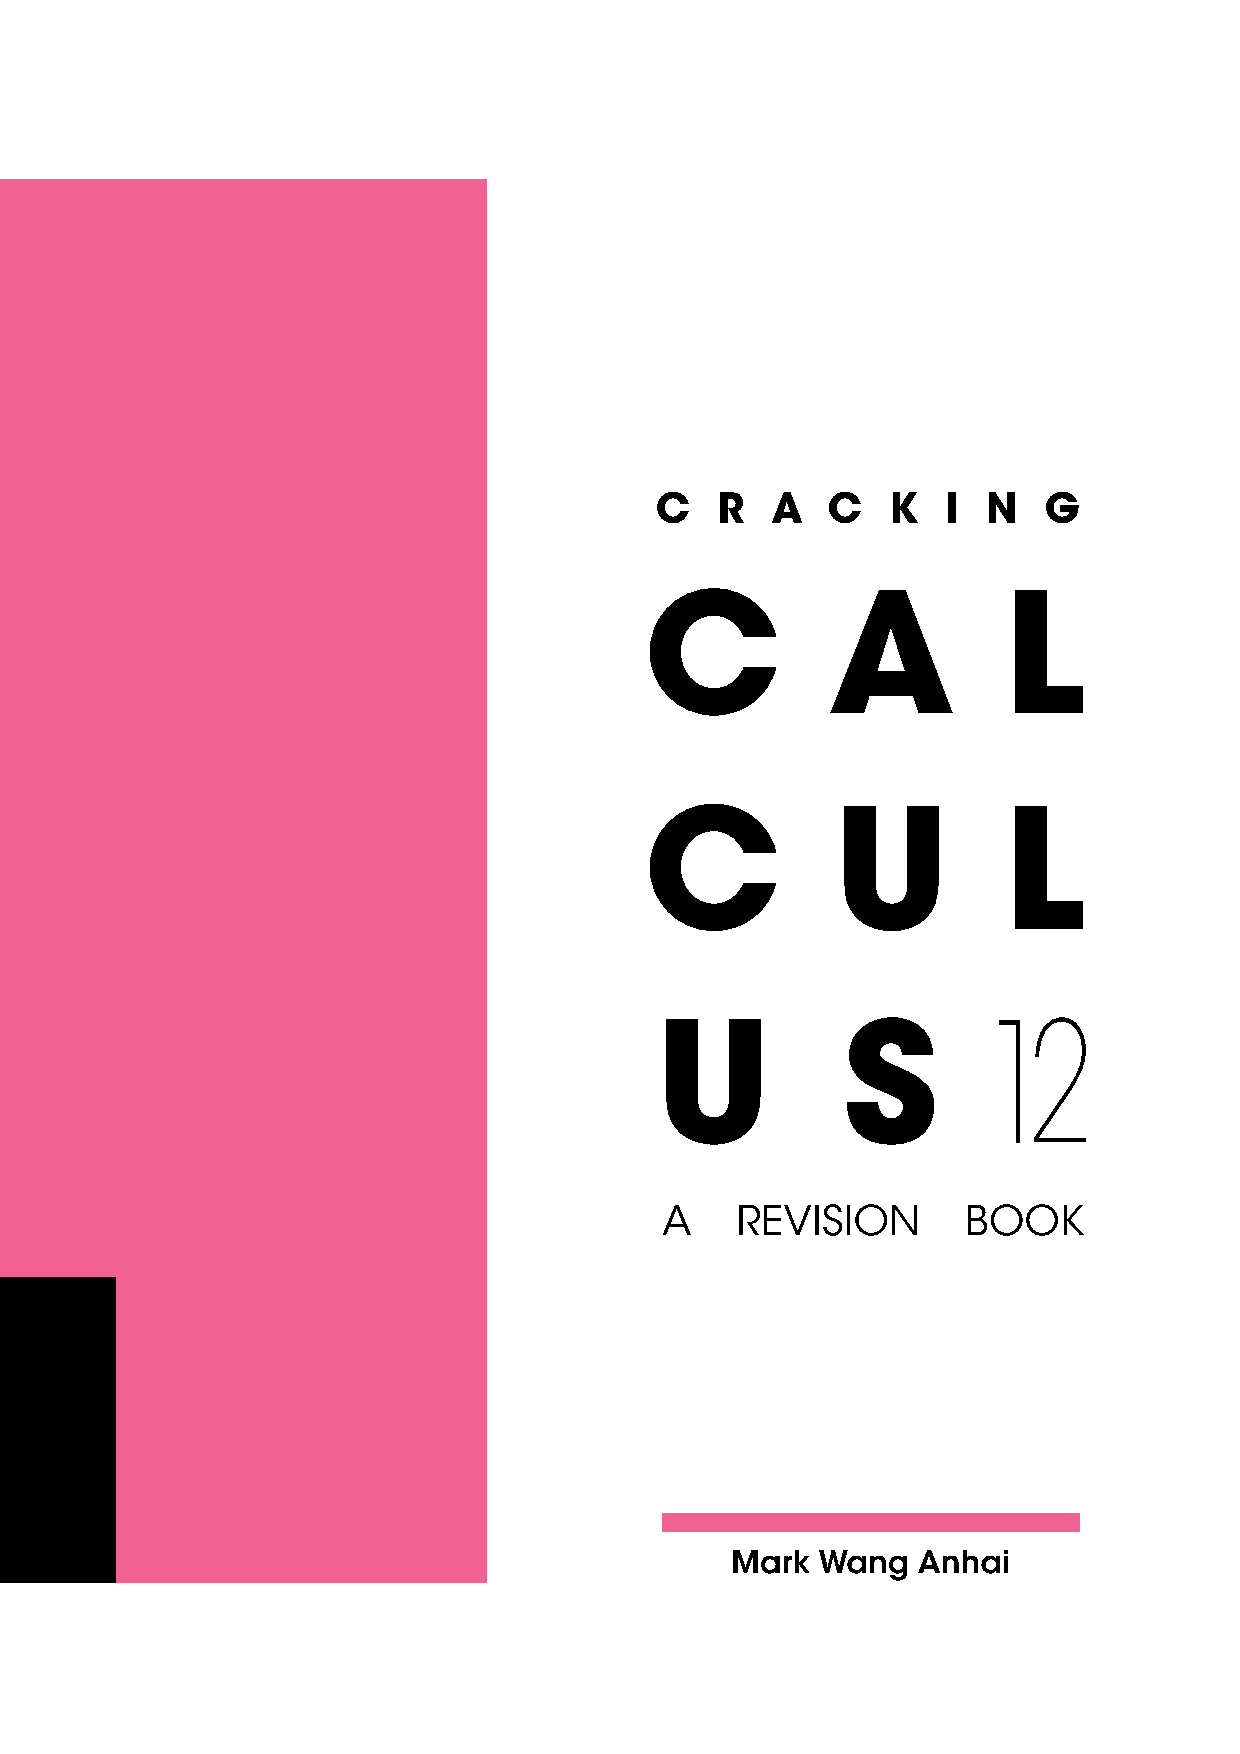
\includegraphics[width=\paperwidth]{img/cover.pdf}};
\end{tikzpicture}
\vfill
\endgroup
    \newpage
~\vfill
\thispagestyle{empty}
\noindent Cracking Calculus 12\\
\noindent Copyright \copyright\ 2019 Mark Wang Anhai\\ % Copyright notice
\noindent \textsc{Created with \LaTeX}\\ % Publisher
\noindent \textsc{MLIS-ZJ Calculus 12 Project}\\\\
\noindent 
    Licensed under the Creative Commons Attribution-NonCommercial 3.0 
    Unported License (the ``License''). You may not use this file except in 
    compliance with the License. You may obtain a copy of the License at 
    \url{http://creativecommons.org/licenses/by-nc/3.0}. Unless required by 
    applicable law or agreed to in writing, software distributed under the 
    License is distributed on an \textsc{``as is'' basis, without warranties 
    or conditions of any kind}, either express or implied. See the License 
    for the specific language governing permissions and limitations under 
    the License.\\ % License information

\noindent
    This text is based on and includes some exercises and examples from the following calculus textbooks: \textit{MOOCulus Calculus} Jim Fowler and Bart Snapp, \textit{Calculus I with Precalculus: Third Edition} by Ron Larson and Bruce H. Edwards, and \textit{Cracking the AP Calculus BC Exam: 2019 Edition} by David S. Khan. \\

\noindent
    The contents in this book are organized in a way that is supplemental to the Maple Leaf International School - Zhenjiang 2019 Calculus 12 curriculum and is intended as a revision material for the course. \\

\noindent
    The theme of this book is based on \textit{The Legrand Orange Book} \LaTeX \text{ }template by Mathias Legrand available at \url{https://www.latextemplates.com/template/the-legrand-orange-book}~under a Creative Commons license. \\

\noindent \textit{First edition, May 2019} % Printing/edition date

    % \usechapterimagefalse % If you don't want to include a chapter image, use this to toggle images off - it can be enabled later with \usechapterimagetrue
\chapterimage{img/wind.jpg} % Table of contents heading image
\pagestyle{empty} % No headers
\tableofcontents % Print the table of contents itself
% \cleardoublepage % Forces the first chapter to start on an odd page so it's on the right
\pagestyle{fancy} % Print headers again
% \usechapterimagetrue
    \part{Prerequisites}
        \chapterimage{img/line.jpg} 
\chapter{Linear and Piecewise Functions}

\section{Introduction to Functions}

Many everyday phenomena involve two quantities that are related to each other by some rule of correspondence. The mathematical term for such a rule of correspondence is a \textbf{relation}. In mathematics, relations are often represented by mathematical equations and formulas. For instance, the simple interest $I$ earned on \$1000 for 1 year is related to the annual interest rate r by the formula $I = 1000r$.  \cite{ci}

The formula $I = 1000r$ represents a special kind of relation that matches each item from one set with \textit{exactly one} item from a different set. Such a relation is called a \textbf{function}.

\begin{definition}[Function]
	A \textbf{function} f from a set $A$ to a set $B$ is a relation that assigns to each element $x$ in the set $A$ exactly one element $y$ in the set $B$. The set $A$ is the \textbf{domain} (or set of inputs) of the function $f$, and the set $B$ contains the \textbf{range} (or set of outputs). \cite{ci}
\end{definition}

Functions are commonlt represented in four ways.

\begin{proposition}[Four ways to represent a function]~\newline
	\begin{enumerate}
		\item \textit{Verbally} by a sentence that describes how the input variable is related to the output variable
		\item \textit{Numerically} by a table or a list of ordered pairs that matches input values with output values
		\item \textit{Graphically} by points on a graph in a coordinate plane in which the input values are represented by the horizontal axis and the output values are represented by the vertical axis
		\item \textit{Analytically} by an equation in two variables
	\end{enumerate}
	\cite{ci}
\end{proposition}

~\newline
To determine whether or not a relation is a function, you must decide whether each input value is matched with exactly one output value. When any input value is matched with two or more output values, the relation is not a function.

\begin{example}[Testing for Functions]~\newline
	Determine whether the relation represents $y$ as a function of $x$. \cite{ci}
	\begin{enumerate}
		\item The input value $x$ is the number of representatives from a state, and the output value $y$ is the number of senators.
		\item Function $f$ is defined as the following table
		      \begin{table}[h]
		      	\centering
		      	\begin{tabular}{l l}
		      		\toprule
		      		\textbf{Input, $x$} & \textbf{Output, $y$} \\
		      		\midrule
		      		2         & 11      \\
		      		2         & 10      \\
		      		3         & 8       \\
		      		4         & 5       \\
		      		5         & 1       \\
		      		\bottomrule
		      	\end{tabular}
		      \end{table}
	\end{enumerate} 
	\begin{solution}~\newline
		\begin{enumerate}
			\item  This verbal description \textit{does} describe $y$ as a function of $x$. Regardless of the value of $x$, the value of $y$ is always 2. Such functions are called \textit{constant functions}.
			\item  This table \textit{does not} describe $y$ as a function of $x$. The input value 2 is matched with two different y-values.
		\end{enumerate}    
	\end{solution}
\end{example}

\section{Function Notation}

When an equation is used to represent a function, it is convenient to name the function so that it can be referenced easily. For example, you know that the equation $y=3x+4$ describes $y$ as a function of $x$. Suppose you give this function the name “$f.$” Then you can use the following \textbf{function notation}. \cite{ci}

\begin{table}[h]
	\centering
	\begin{tabular}{l l l}
		\toprule
		\textbf{Input} & \textbf{Output} & \textbf{Equation} \\
		\midrule
		$x$   & $f(x)$    & $f(x) = 3x+4$ \\
		\bottomrule
	\end{tabular}
\end{table}

The symbol $f(x)$ is read as the value of $f$ at $x$ or simply $f$ of $x$. The symbol $f(x)$ corresponds to the y-value for a given $x$. So, you can write $y=f(x)$. Keep in mind that $f$ is the name of the function, whereas $f(x)$ is the value of the function at $x$. For instance, the function given by
\begin{align}
	  & f(x) = 3x+4 
\end{align}

has function values denoted by $f(0)$, $f(1)$, $f(2)$, and so on. To find these values, substitute the specified input values into the given equation.
\begin{align*}
	f(-1) & =3(-1)+4 = -3+4 = 1 &   & x=-1 \\
	f(0)  & =3(0)+4 = 0+4 = 4   &   & x=0  \\
	f(2)  & =3(2)+4 = 6+4 = 10  &   & x=2  
\end{align*}

Although $f$ is often used as a convenient function name and $x$ is often used as the independent variable, you can use other letters. For instance,
\begin{align}
	  & f(x)=3x+4\text{, }\quad f(t)=3t+4\text{, }\quad g(s)=3s+4 
\end{align}

all define the same function. In fact, the role of the independent variable is that of a “placeholder” that can be replaced by 
\textit{any real number or algebraic expression}. \cite{ci}

\begin{example}[Evaluating a Function]~\newline
	Let $g(x)=-7x+20$. Find each function value \cite{ci}
	\begin{enumerate}
		\item $g(2)$
		\item $g(t)$
		\item $g(x+2)$\\
	\end{enumerate} 
	\begin{solution}~\newline
		\begin{enumerate}
			\item  Replacing $x$ with 2 in $g(x)=-7x+20$ yields the following.
			      \begin{align}
			      	g(2) & = -7(2) + 20 \\
			      	     & = -14+20     \\
			      	     & = 6          
			      \end{align}
			\item  Replacing $x$ with $t$ yields the following.
			      \begin{align}
			      	g(t) & = -7(t) + 20 \\
			      	     & = -7t+20     
			      \end{align}
			\item  Replacing $x$ with $x+2$ yields the following.
			      \begin{align}
			      	g(x+2) & = -7(x+2) + 20 \\
			      	       & = -7x-14+20    \\
			      	       & =7x+20         
			      \end{align}
		\end{enumerate}    
	\end{solution}
\end{example}

\section{Piecewise Function}
A function defined by two or more equations over a specified 
domain is called a \textbf{piecewise-defined function}. \cite{ci}\\

\begin{example}[A Piecewise-Defined Function]~\newline
	Evaluate the function when $x=-1$, $0$, and $1$. \cite{ci}
	\begin{equation}
		f(x)=\left\{
		\begin{aligned} 
			  & x^2+1, &   & x < 0    \\
			  & x-1,   &   & x \geq 0
		\end{aligned}\right.
	\end{equation}
	\begin{solution} Because $x=-1$ is less than 0, use $f(x)=x^2+1$ 
		to obtain
		\begin{align}f(-1) = (-1)^2+1 = 2\end{align}
		For $x=0$, use $f(x) = x-1$ to obtain
		\begin{align}f(0) = (0)-1 = -1\end{align}
		For $x=1$, use $f(x) = x-1$ to obtain
		\begin{align}f(1) = (1)-1 = 0\end{align}
	\end{solution}
\end{example}


\begin{exercise}
    ~\\

    \begin{enumerate} 
		\item A relation that assigns to each element x from a set of inputs, or \blank, exactly one element y in a set of outputs, or \blank, is called a \blank. \cite{ci}
		\item Functions are commonly represented in four different ways, \blank, \blank, \blank, and \blank. \cite{ci}
		\item For an equation that represents y as a function of x, the set of all values taken on by the \blank variable x is the domain, and the set of all values taken on by the \blank variable y is the range. \cite{ci}
        \item The function given by\\
		$f(x)=
		\begin{cases}
			2x-1,	& x<0\\
			x^2+4,	& x\geq 0
		\end{cases}$\\
		is an example of a \blank function.
    \end{enumerate}
    ~\\\-\hspace{0.3cm} \textbf{
        In Exercises 5–7, evaluate the function at each specified value of the independent variable and simplify.
    }\\
    \begin{enumerate}
        \setcounter{enumi}{4}
        \item $f(x)=2x-3$\\
        (a) $f(1)$ \qquad (b) $f(-3)$ \qquad (c) $f(x-1)$
        \item $f(x)=
		\begin{cases}
			3x-1,	& x<-1				\\
			4,		& -1 \leq x \leq 1	\\
			x^2,	& x>1
		\end{cases}$\\
        (a) $f(-2)$ \qquad (b) $f(-\dfrac{1}{2})$ \qquad (c) $f(3)$
        \item $f(x)=
		\begin{cases}
			4-5x,	& x\leq -2		\\
			0,		& -2 < x < 2	\\
			x^2+1,	& x\geq 2
		\end{cases}$\\
        (a) $f(-3)$ \qquad (b) $f(4)$ \qquad (c) $f(-1)$
    \end{enumerate}

\end{exercise}

        \chapterimage{img/step.jpg} 
\chapter{Polynomial and Rational Functions}
\section{Quadratic Function}

In this and the next section, you will study the graphs of polynomial functions. In Chapter 1, you were introduced to the following basic functions. \cite{ci}

\begin{align*}
    f(x)&=ax+b       && \text{Linear function}\\
    f(x)&=c          && \text{Constant function}\\
    f(x)&=x^2        && \text{Squaring function}\\
\end{align*}

These functions are examples of \textbf{polynomial functions}.

\begin{definition}[Polynomial Function]
    Let n be a nonnegative integer and let $a_n, a_{n-1}, \dddot{} , a_2, \\a_1, a_0$ be real numbers with $a_n \neq 0$. The function given by
    $$f(x)=a_nx^n+a_{n-1}x^{n-1}+\dddot{}+a_2x^2+a_1x+a_0$$
    is called a \textbf{polynomial function of $x$ with degree $n$}.
    \\ \cite{ci}
\end{definition}

Polynomial functions are classified by degree. For instance, a constant function $f(x)=c$ with $c\neq 0$ has degree 0, and a linear function $f(x)=ax+b$ with $a\neq 0$ has degree 1. In this section, you will study second-degree polynomial functions, which are called \textbf{quadratic functions}. \cite{ci}

For instance, each of the following functions is a quadratic function.
\begin{align*}
    f(x)&=x^2+6x+2\\
    g(x)&=2(x+1)^2-3\\
    h(x)&=9+\dfrac{1}{4}x^2\\
    k(x)&=-3x^2+4\\
    m(x)&=(x-2)(x+1)\\
\end{align*}
Note that the squaring function is a simple quadratic function that has degree 2.

\begin{definition}[Quadratic Function]
    Let $a$, $b$, and $c$ be real numbers with $a \neq 0$. The function given by $$f(x)=ax^2+bx+c$$
    is called a \textbf{quadratic function}.
    \\ \cite{ci}
\end{definition}

The graph of a quadratic function is a special type of “U”-shaped curve called a \textbf{parabola}. Parabolas occur in many real-life applications—especially those involving reflective properties of satellite dishes and flashlight reflectors.

All parabolas are symmetric with respect to a line called the \textbf{axis of symmetry}, or simply the \textbf{axis} of the parabola. The point where the axis intersects the parabola is the \textbf{vertex} of the parabola, as shown in Figure \ref{plot:quat func bas}. When $a > 0$, the graph of
$$f(x)=ax^2+bx+c$$
is a parabola that opens upward. When $a < 0$, the graph of
$$f(x)=ax^2+bx+c$$
is a parabola that opens downward. \cite{ci}

\begin{figure}[H]
    \centering
    \begin{multicols}{2}
    \begin{tikzpicture}
        \begin{axis}[nejes=-6:2 -2:10,xlabel=$x$, ylabel=$y$]
            \addplot [domain=-10:5, very thick, black] {(x+2)^2+2};
            \addplot [soldot, black] coordinates{(-2,2)} node[left=1.6cm, below,pos=1,black] {Vertex is minimum};
            \draw[dashed, penColor, thick] (axis cs:-2,-2) -- (axis cs:-2,8) node[above,pos=1,black] {Opens upward};
        \end{axis}
    \end{tikzpicture}
    $a > 0$
    \begin{tikzpicture}
        \begin{axis}[nejes=-6:2 -2:10,xlabel=$x$, ylabel=$y$]
            \addplot [domain=-20:5, very thick, black] {-(x+2)^2+8};
            \addplot [soldot, black] coordinates{(-2,8)} node[left=1.6cm, above,pos=1,black] {Vertex is maximum};
            \draw[dashed, penColor, thick] (axis cs:-2,10) -- (axis cs:-2,-1) node[below,pos=1,black] {Opens downward};
        \end{axis}
    \end{tikzpicture}
    $a < 0$
\end{multicols}
    \caption{Parabola of $ax^2+bx+c$}
    \label{plot:quat func bas}
\end{figure}

The simplest type of quadratic function is
$$f(x)=ax^2$$
Its graph is a parabola whose vertex is (0, 0). When $a$ > 0, the vertex is the point with the \textit{minimum} $y$-value on the graph, and when $a$ < 0, the vertex is the point with the \textit{maximum} $y$-value on the graph, as shown in Figure \ref{plot:quat func bas}. \cite{ci}

\section{Polynomial Functions of Higher Degree}

In this section, you will study basic features of the graphs of polynomial functions. The first feature is that the graph of a polynomial function is \textit{continuous}. Essentially, this means that the graph of a polynomial function has no breaks, holes, or gaps, as shown in Figure \ref{plot:polynomials are countinuous}(a). The graph shown in Figure \ref{plot:polynomials are countinuous}(b) is an example of a piecewise-defined function that is not continuous.

\begin{figure}[H]
    \centering
    \begin{multicols}{2}
    \begin{tikzpicture}
        \begin{axis}[nejes=-1:5 -1:5,xlabel=$x$, ylabel=$y$, height=4cm]
            \addplot [domain=-1:5, very thick, penColor] {(x-1)^3-x+3};
        \end{axis}
    \end{tikzpicture}
    (a) Polynomial functions have continuous graphs.
    \begin{tikzpicture}
        [
            declare function={
                func(\x)= (\x < 3) * -(x-2)^2+3   +
                (\x > 3) * (x-3)^2+1
            ;
        }]
        \begin{axis}[nejes=-1:10 -2:8,xlabel=$x$, ylabel=$y$, height=4cm]
            \addplot [domain=-1:3, very thick, penColor] {func(x)};
            \addplot [domain=3:8, very thick, penColor] {func(x)};
            \addplot [holdot] coordinates{(3,3)};
            \addplot [soldot] coordinates{(3,4)};
        \end{axis}
    \end{tikzpicture}
    (b) Functions with graphs that are not continuous are not polynomial functions.
\end{multicols}
    \caption{Continuity of Polynomial Functions}
    \label{plot:polynomials are countinuous}
\end{figure}

The second feature is that the graph of a polynomial function has only smooth, rounded turns, as shown in Figure \ref{plot:polynomials are smooth}(a). A polynomial function cannot have a sharp turn. For instance, the function given by $f(x)=|x|$, which has a sharp turn at the point (0, 0), as shown in Figure \ref{plot:polynomials are smooth}(b), is not a polynomial function.

\begin{figure}[H]
    \centering
    \begin{multicols}{2}
    \begin{tikzpicture}
        \begin{axis}[nejes=-4:4 -2:2,xlabel=$x$, ylabel=$y$, height=4cm]
            \addplot [domain=-4:4, very thick, penColor] {x^5-2*x^3};
        \end{axis}
    \end{tikzpicture}
    (a) Polynomial functions have graphs with smooth, rounded turns.
    \begin{tikzpicture}
        \begin{axis}[ejes=-4:4 -1:4,xlabel=$x$, ylabel=$y$, height=4cm]
            \addplot [domain=-4:4, very thick, penColor] {abs(x)};
            \addplot [soldot] coordinates{(0,0)};
        \end{axis}
    \end{tikzpicture}
    (b) Graphs of polynomial functions
    cannot have sharp turns.
\end{multicols}
    \caption{Smoothness of Polynomial Functions}
    \label{plot:polynomials are smooth}
\end{figure}

\section{Real Zeros of Polynomial Functions}

It can be shown that for a polynomial function $f$ of degree $n$, the following statements are true. \cite{ci}
\begin{enumerate}
    \item The function $f$ has, at most, $n$ real zeros. 
    \item The graph of $f$ has, at most, $n-1$ turning points.
\end{enumerate}
~\\
\begin{proposition}[Real Zeros of Polynomial Functions ]\cite{ci}
    ~\\
    When $f$ is a polynomial function and $a$ is a real number, the following statements are equivalent.
    \begin{enumerate}
        \item $x=a$ is a \textit{zero} of the function $f$.
        \item $x=a$ is a solution of the polynomial equation $f(x)=0$. 
        \item $(x-a)$ is a factor of the polynomial $f(x)$.
        \item $(a,0)$ is an x-intercept of the graph of $f$.
    \end{enumerate}
\end{proposition}
~\\
\begin{example}[Find the Zeros of a Polynomial Function ]\cite{ci}~\newline
    Find all real zeros of
    $$f(x)=-2x^4+2x^2.$$
    Then determine the number of turning points of the graph of the function.\\
    \begin{solution}~\newline
        To find the real zeros of the function, set $f(x)$ equal to zero and solve for $x$.
        \begin{align*}
            -2x^4+2x^2      & = 0   && \text{Set $f(x)$ equal to 0.}\\
            -2x^2(x^2-1)    & = 0   && \text{Remove common monomial factor.}\\
            -2x^2(x-1)(x+1) & = 0   && \text{Factor completely.}
        \end{align*}
        So, the real zeros are $x = 0$, $x = 1$, and $x = -1$. Because the function is a fourth-degree polynomial, the graph of $f$ can have at most $4 - 1 = 3$ turning points.\\
	\end{solution}
\end{example}

\begin{proposition}[Repeated Zeros ]\cite{ci}
    ~\\
    A factor $(x-a)^k, k>1$, yields a \textbf{repeated zero} $x=a$ of \textbf{multiplicity} $k$.
    \begin{enumerate}
        \item When $k$ is odd, the graph \textit{crosses} the $x$-axis at $x=a$.
        \item When $k$ is even, the graph \textit{touches} the $x$-axis (but does not cross the $x$-axis) at $x=a$.
    \end{enumerate}
\end{proposition}

\section{Rational Functions}

A rational function is a quotient of polynomial functions. It can be written in the form
$$f(x)=\dfrac{N(x)}{D(x)}$$
where $N(x)$ and $D(x)$ are polynomials and $D(x)$ is not the zero polynomial.\cite{ci}

In general, the \textit{domain} of a rational function of $x$ includes all real numbers except $x$-values that make the denominator zero. Much of the discussion of rational functions will focus on their graphical behavior near these $x$-values excluded from the domain. \cite{ci}

\section{Vertical and Horizontal Asymptotes}

Consider this function:
$$f(x) = \dfrac{1}{x}$$

\begin{figure}[H]
    \centering
    \begin{tikzpicture}
        \begin{axis}[
                ejes=-2:2 -2:2,xlabel=$x$, ylabel=$y$,
                every axis y label/.style={at=(current axis.above origin),anchor=south},
                every axis x label/.style={at=(current axis.right of origin),anchor=west},
            ]
            \addplot [domain=0:2, very thick, penColor] {1/x};
            \addplot [domain=-2:0, very thick, penColor] {1/x};
        \end{axis}
    \end{tikzpicture}
    \caption{A plot of $\dfrac{1}{x}$.}
    \label{plot:1/x}
\end{figure}

the behaviour of $f$ near $x=0$ is denoted as follows.
$$
f(x) \to -\infty \text{ as } x \to 0^- 
\qquad
f(x) \to \infty \text{ as } x \to 0^+
$$
The line $x=0$ is a \textbf{vertical asymptote} of the graph of $f$, as shown in Figure \ref{plot:1/x}. From
this figure, you can see that the graph of $f$ also has a \textbf{horizontal asymptote} — the line $y=0$. This means that the values of $f(x)=\dfrac{1}{x}$ approach zero as $x$ increases or decreases without bound.
$$
f(x) \to 0 \text{ as } x \to -\infty 
\qquad
f(x) \to 0 \text{ as } x \to \infty
$$

\begin{definition}[Vertical and Horizontal Asymptotes]
    ~\\ 
    \begin{enumerate}
        \item The line $x=a$ is a \textbf{vertical asymptote} of the graph of $f$ when
        $$f(x) \to -\infty \text{ or } f(x) \to \infty$$
        as $x\to a$, either from the right or from the left.
        \item The line $y=b$ is a \textbf{horizontal asymptote} of the graph of $f$ when
        $$f(x) \to b$$
        as $x\to \infty$ or $x\to -\infty$. 
    \end{enumerate}
    \cite{ci}   
\end{definition}
\clearpage
\begin{proposition}[Vertical and Horizontal Asymptotes of a Rational Function]\cite{ci}
    ~\\
    Let $f$ be the rational function given by
    $$f(x)=\dfrac{N(x)}{D(x)} = \dfrac
    {a_nx^n+a_{n-1}x^{n-1}+ \dddot{} +a_1x+a_0}
    {b_mx^m+b_{m-1}x^{m-1}+ \dddot{} +b_1x+b_0}$$ 
    where $N(x)$ and $D(x)$ have no common factors.
    \begin{enumerate}
        \item The graph of $f$ has \textit{vertical} asymptotes at the zeros of $D(x)$.
        \item The graph of $f$ has one or no \textit{horizontal} asymptote determined by comparing the degrees of $N(x)$ and $D(x)$.
        \begin{enumerate}
            \item When $n < m$,the graph of $f$ has the line $y=0$ (the $x$-axis) as a horizontal asymptote.
            \item When $n = m$,the graph of $f$ has the line $y=\dfrac{a_n}{b_m}$ (ratio of the leading coefficients) as a horizontal asymptote.
            \item When $n > m$,the graph of $f$ has no horizontal asymptote.
        \end{enumerate}
    \end{enumerate}
\end{proposition}
~\\
\begin{example}[Finding Vertical and Horizontal Asymptotes]\cite{ci}~\newline
    Find all vertical and horizontal asymptotes of the graph of each rational function.
    \begin{enumerate}
        \item $f(x)=\dfrac{2x^2}{x^2-1}$
        \item $f(x)=\dfrac{x^2+x-2}{x^2-x-6}$
    \end{enumerate}
    ~\\
    \begin{solution}~\newline
        \begin{enumerate}
            \item For this rational function, the degree of the numerator is equal to the degree of the denominator. The leading coefficient of the numerator is 2 and the leading coefficient of the denominator is 1, so the graph has the line $y=2$ as a horizontal asymptote. To find any vertical asymptotes, set the denominator equal to zero and solve the resulting equation for $x$.
            \begin{align*}
                x^2-1 &=0       &&\text
                {Set denominator equal to zero.}\\
                (x+1)(x-1)&=0   &&\text
                {Factor.}\\
                x+1&=0,\quad x=-1    &&\text
                {Set 1st factor equal to 0.}\\
                x-1&=0,\quad x=1     &&\text
                {Set 2nd factor equal to 0.}
            \end{align*}
            This equation has two real solutions, $x=1$ and $x=-1$, so the graph has the lines $x=1$ and $x=-1$ as vertical asymptotes.

            \item For this rational function, the degree of the numerator is equal to the degree of the denominator. The leading coefficient of both the numerator and denominator is 1, so the graph has the line $y=1$ as a horizontal asymptote. To find any vertical asymptotes, first factor the numerator and denominator as follows.
            $$f(x)=\dfrac{x^2+x-2}{x^2-x-6}=\dfrac{(x-1)(x+2)}{(x+2)(x-3)}=\dfrac{x-1}{x-3},\quad x\neq -2$$
            By setting the denominator $x-3$ (of the simplified function) equal to zero, you can determine that the graph has the line $x=3$ as a vertical asymptote.
        \end{enumerate}
	\end{solution}
\end{example}

\begin{exercise}
    ~\\\-\hspace{0.3cm} \textbf{
        In Exercises 1–4, (a) find all the real zeros of the polynomial function, (b) determine the multiplicity of each zero and the number of turning points of the graph of the function.
    }\cite{ci}\\
    \begin{enumerate} 
		\item $f(x) = x^2-36$
		\item $g(x) = 3x^3-12x^2+3x$
		\item $f(c) = 3x^3+3x^2-4x-12$
		\item $f(t) = t^5-6t^3+9t$
    \end{enumerate}
    ~\\\-\hspace{0.3cm} \textbf{
        In Exercises 5–8, find a polynomial function that has the given zeros. (There are many correct answers.)
    }\cite{ci}\\
    \begin{enumerate}
        \setcounter{enumi}{4}
        \item $0,8$
        \item $4,-3,3,0$
        \item $1+\sqrt{3}, 1-\sqrt{3}$
        \item $0, -4, -5$
    \end{enumerate}
    ~\\\-\hspace{0.3cm} \textbf{
        In Exercises 9–12, find any vertical and horizontal Asymptotes.
    }\cite{ci}\\
    \begin{enumerate}
        \setcounter{enumi}{8}
        \item $f(x)=-\dfrac{1}{(x-2)^2}$
        \item $f(x) = \dfrac{2x^2-5x-3}{x^3-2x^2-5x+6}$
        \item $f(x) = \dfrac{x^2+3x)}{x^2+x-6}$
        \item $f(t) = \dfrac{t^2-1}{t-1}$
    \end{enumerate}
\end{exercise}

        \chapterimage{img/comb.jpg} 
\chapter{Combination of Functions}
\section{Arithmetic Combinations of Functions}
Just as two real numbers can be combined by the operations of addition, subtraction, multiplication, and division to form other real numbers, two functions can be combined to create new functions. For example, the functions given by $f(x)=2x-3$ and $g(x)=x^2-1$ can be combined to form the sum, difference, product, and quotient of $f$ and $g$. \cite{ci}

\begin{align*}
    f(x)+g(x)   &=  (2x-3)+(x^2-1)\\
                &=  x^2+2x+4        &&\text{Sum}\\
    f(x)-g(x)   &=  (2x-3)-(x^2-1)\\
                &=  -x^2+2x-2       &&\text{Difference}\\
    f(x)g(x)    &=  (2x-3)(x^2-1)\\
                &=  2x^3-3x^2-2x+3  &&\text{Product}\\
    \dfrac{f(x)}{g(x)}   &=  \dfrac{2x-3}{x^2-1}, \qquad x\neq \pm 1      &&\text{Quotient}
\end{align*}

The domain of an \textbf{arithmetic combination} of functions $f$ and $g$ consists of all real numbers that are common to the domains of $f$ and $g$. In the case of the quotient $\dfrac{f(x)}{g(x)}$, there is the further restriction that $g(x)\neq 0$. \cite{ci}

\begin{example}[Finding the Sum of Two Functions] \cite{ci}~\\
    Given $f(x)=2x+1$ and $g(x)=x^2+2x-1$, find $(f+g)(x)$. Then evaluate the sum when $x=3$.\\
    \begin{solution}
        $$(f+g)(x) = f(x)+g(x) = (2x+1) + (x^2+2x-1) = x^2+4x$$
        When $x = 3$, the value of this sum is
        $$(f+g)(3) = (3)^2+4(3)  =21.$$
    \end{solution}
\end{example}
\begin{example}[Finding the Difference of Two Functions] \cite{ci}~\\
    Given $f(x)=2x+1$ and $g(x)=x^2+2x-1$, find $(f-g)(x)$. Then evaluate the sum when $x=2$.\\
    \begin{solution}
        $$(f-g)(x) = f(x)-g(x) = (2x+1) - (x^2+2x-1) = -x^2+2$$
        When $x = 2$, the value of this sum is
        $$(f-g)(3) = -(2)^2+2  =-1.$$
    \end{solution}
\end{example}
\begin{example}[Finding the Product of Two Functions] \cite{ci}~\\
    Given $f(x)=x^2$ and $g(x)=x-3$, find $(fg)(x)$. Then evaluate the sum when $x=4$.\\
    \begin{solution}
        $$(fg)(x) = f(x)g(x) = (x^2)(x-3) = x^3-3x^2$$
        When $x = 3$, the value of this sum is
        $$(fg)(4) = (4)^3-3(4)^2  =16.$$
    \end{solution}
\end{example}
\begin{example}[Finding the Quotients of Two Functions] \cite{ci}~\\
    Given $f(x)=\sqrt{x}$ and $g(x)=\sqrt{4-x^2}$, find $(f/g)(x)$ and $(g/f)(x)$. Then find the domains of $f/g$ and $g/f$\\
    \begin{solution}
        The quotient of $f$ and $g$ is
        $$\left(\dfrac{f}{g}\right)(x) = \dfrac{f(x)}{g(x)} = \dfrac{\sqrt{x}}{\sqrt{4-x^2}}$$
        and the quotient of $g$ and $f$ is 
        $$\left(\dfrac{g}{f}\right)(x) = \dfrac{g(x)}{f(x)} = \dfrac{\sqrt{4-x^2}}{\sqrt{x}}$$
        The domain of $f$ is $[0,\infty)$ and the domain of $g$ is $[2,-2]$. The intersection of these domains is $[0,2]$. So, the domains of $f/g$ and $g/f$ are as follows.
        $$\text{Domain of }\dfrac{f}{g}: [0,2) 
        \qquad
        \text{Domain of }\dfrac{g}{f}: (0,2] $$
    \end{solution}
\end{example}

\section{Composition of Functions}

\begin{definition}[Composition of Two Functions] 
    The \textbf{composition} of the function $f$ with the function $g$ is
    $$(f\circ g)(x)=f(g(x)).$$
    The domain of $f\circ g$ is the set of all $x$ in the domain of $g$ such that $g(x)$ is in the domain of $f$. (See Figure \ref{fig:domain_comp}.)
    \\\cite{ci}
\end{definition}

\begin{figure}[h]
\centering
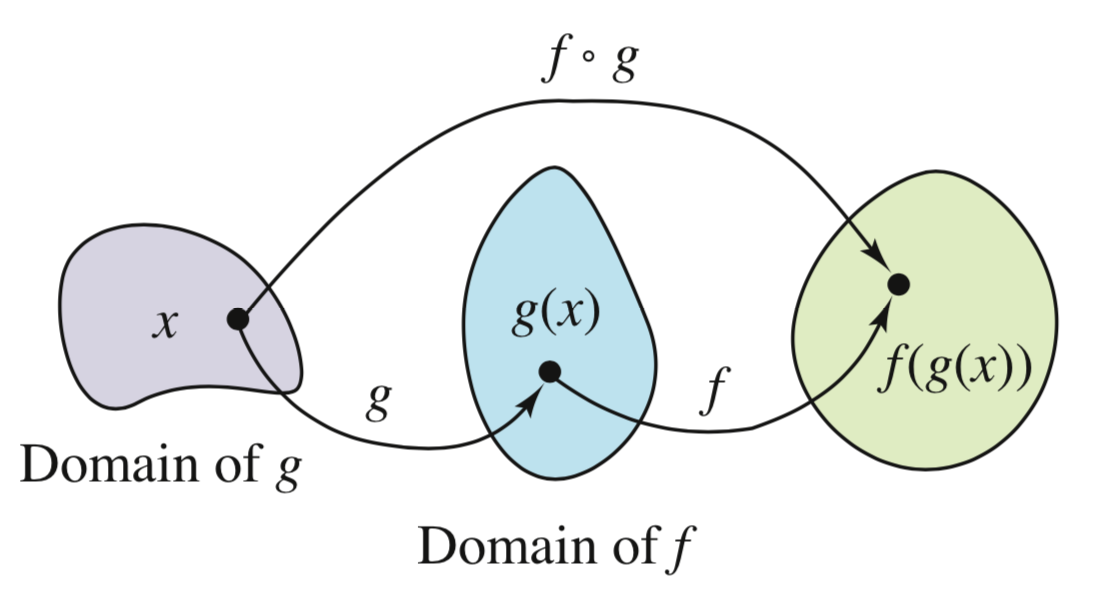
\includegraphics[scale=0.5]{img/fig/domain_comp.png}
\caption{Domain of a Composition Function \cite{ci}}
\label{fig:domain_comp}
\end{figure}

\begin{example}[Composition of Functions] \cite{ci}~\\
    Given $f(x)=x+2$ and $g(x)=4-x^2$, find the following.
    \begin{enumerate}
        \item $(f\circ g)(x)$ 
        \item $(g\circ f)(x)$
        \item $(g\circ f)(-2)$ 
    \end{enumerate}~\\
    \begin{solution}~\\
        \begin{enumerate}
            \item The composition of $f$ with $g$ is as follows.
            \begin{align*}
                (f\circ g)(x) &= f(g(x))\\
                &=f(4-x^2)
                &=(4-x^2)+2
                &=-x^2+6
            \end{align*}
            \item The composition of $g$ with $f$ is as follows.
            \begin{align*}
                (g\circ f)(x) &= g(f(x))\\
                &=g(x+2)
                &=4-(x+2)^2
                &=-x^2-4x
            \end{align*}
            Note that, in this case, $(f\circ g)(x)\neq (g\circ f)(x)$.
            \item Using the result of part 2, you can write the following.
            \begin{align*}
                (g\circ f)(-2) &=-(-2)^2-4(-2)
                &= -4+8
                &= 4
            \end{align*}
        \end{enumerate}
    \end{solution}
\end{example}

\section{Application}

\begin{example}[Bacteria Count] \cite{ci}~\\
    The number $N$ of bacteria in a refrigerated food is given by
    $$N(T)=20T^2-80T+500, \qquad 2\leq T \leq 14$$
    where $T$ is the temperature of the food in degrees Celsius. When the food is removed from refrigeration, the temperature of the food is given by
    $$T(t)=4t+2, \qquad 0\leq t\leq 3$$
    where $t$ is the time in hours.
    \begin{enumerate}
        \item Find the composition $N(T(t))$ and interpret its meaning in context.
        \item Find the time when the bacteria count reaches 2000.
    \end{enumerate}
    ~\\
    \begin{solution}~\\
        \begin{enumerate}
            \Item \begin{align*}
                N(T(t)) 
                &= 20(4t+2)^2-80(4t+2)+500\\
                &= 20(16t^2+16t+4)-320t-160+500\\
                &= 320t^2+320t+80-320t-160+500\\
                &= 320t^2+420
            \end{align*}
            The composite function $N(T(t))$ represents the number of bacteria in the food as a function of the amount of time the food has been out of refrigeration.
            \item The bacteria count will reach 2000 when $320t^2+420=2000$. Solve this equation for $t$ as shown.
            \begin{align*}
                320t^2+420 &= 2000\\
                320t^2 &= 1580\\
                t^2 &= \dfrac{79}{16}\\
                t &= \dfrac{\sqrt{79}}{4}\\
                t &\approx 2.2
            \end{align*}
            So, the count will reach 2000 when $t\approx 2.2$ hours.
            When you solve this equation, note that the negative value is rejected because it is not in the domain of the composite function.
        \end{enumerate}
    \end{solution}
\end{example}

\begin{exercise}
    ~\\\-\hspace{0.3cm} \textbf{
        In Exercises 1–2, find (a) $(f+g)(x)$, (b) $(f-g)(x)$, (c) $(fg)(x)$, and (d) $(f/g)(x)$.
    }\cite{ci}\\
    \begin{enumerate} 
		\item $f(x) = x^2,\quad g(x)=4x-5$
		\item $f(x) = \dfrac{1}{x},\quad g(x)=\dfrac{1}{x^2}$
    \end{enumerate}
    ~\\\-\hspace{0.3cm} \textbf{
        In Exercises 3–5, evaluate the indicated function for
        $f(x)=x^2+1$ and $g(x)=x-4$.
    }\cite{ci}\\
    \begin{enumerate}
        \setcounter{enumi}{2}
        \item $(f+g)(2)$
        \item $(fg)(6)$
        \item $(f/g)(-1)-g(3)$
    \end{enumerate}
    % ~\\\-\hspace{0.3cm} \textbf{
    %     In Exercises 7–10, find any vertical and horizontal Asymptotes.
    % }\cite{ci}\\
    % \begin{enumerate}
    %     \setcounter{enumi}{8}
    %     \item $f(x)=-\dfrac{1}{(x-2)^2}$
    %     \item $f(x) = \dfrac{2x^2-5x-3}{x^3-2x^2-5x+6}$
    %     \item $f(x) = \dfrac{5(x+4)}{x^2+x-12}$
    %     \item $f(x) = \dfrac{1-2x}{x}$
    % \end{enumerate}
\end{exercise}

        \chapterimage{img/inv.jpg} 
\chapter{Inverse Functions}
\section{Inverse Functions}
Recall that a function can be represented by a set of ordered pairs. For instance, the function $f(x)=x+4$ from the set $A ={1, 2, 3, 4}$ to the set $B = {5, 6, 7, 8}$ can be written as follows. \cite{ci}
$$f(x) = x+4: {(1,5),(2,6),(3,7),(4,8)}$$
In this case, by interchanging the first and second coordinates of each of these ordered pairs, you can form the \textbf{inverse function} of $f$, which is denoted by $f^{-1}$. It is a function from the set $B$ to the set $A$, and can be written as follows. \cite{ci}
$$f^{-1}(x) = x-4: {(5,1),(6,2),(7,3),(8,4)}$$
Note that the domain of $f$ is equal to the range of $f^{-1}$, and vice versa, as shown in Figure \ref{fig:domain_inv}. Also note that the functions $f$ and $f^{-1}$ have the effect of “undoing” each other. In other words, when you form the composition of $f$ with $f^{-1}$ or the composition of $f^{-1}$ with $f$, you obtain the identity function. \cite{ci}

$$f(f^{-1}(x))=f(x-4)=(x-4)+4=x$$
$$f^{-1}(f(x))=f^{-1}(x+4)=(x+4)-4=x$$

\begin{figure}[H]
    \centering
    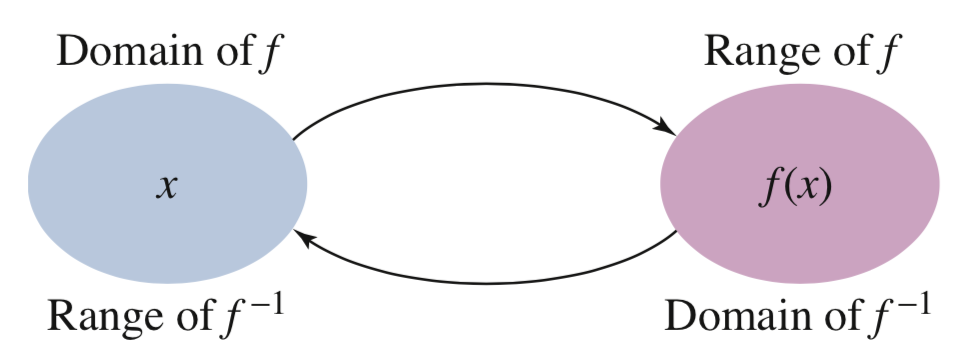
\includegraphics[scale=0.5]{img/fig/domain_inv.png}
    \caption{Domain of an Inverse Function \cite{ci}}
    \label{fig:domain_inv}
\end{figure}

\begin{definition}
    Let $f$ and $g$ be two functions such that
    $$f(g(x))=x\qquad \text{for every $x$ in the domain of $g$}$$
    and
    $$g(f(x))=x\qquad \text{for every $x$ in the domain of $f$}$$
    Under these conditions, the function $g$ is the \textbf{inverse function} of the function $f$. The function $g$ is denoted by $f^{-1}$ (read “f-inverse”). 
    \\\cite{ci}
\end{definition}

If the function $g$ is the inverse function of the function $f$, it must also be true that the function $f$ is the inverse function of the function $g$. For this reason, you can say that the functions $f$ and $g$ are \textit{inverse functions of each other}.

\section{The Graph of an Inverse Function}
The graphs of a function $f$ and its inverse function $f^{-1}$ are related to each other in the following way. If the point $(a,b)$ lies on the graph of $f$, then the point $(b,a)$ must lie on the graph of $f^{-1}$, and vice versa. This means that the graph of $f^{-1}$ is a reflection of the graph of $f$ in the line $y = x$, as shown in Figure \ref{plot:inv func}.

\begin{figure}[H]
    \centering
    \begin{tikzpicture}
        \begin{axis}[
                nejes=-3:3 -3:3,xlabel=$x$, ylabel=$y$
            ]
            \addplot [very thick, penColor, smooth] {x^3} node[pos=0.7, above left, black] {$f(x)$};
            \addplot [very thick, penColor2, smooth] {x/abs(x)*abs(x)^(1/3)} node[pos=0.8, below right, black] {$f^{-1}(x)$};
            \draw[dashed, black, thick] (axis cs:-3,-3) -- (axis cs:3,3);
            \draw[dashed, black, thick] (axis cs:-2,-1.2599210499) -- (axis cs:-1.2599210499,-2);
            \addplot [soldot, black] coordinates{(-2,-1.2599210499)} node[pos=-0.2, above left,black] {$(b,a)$};
            \addplot [soldot, black] coordinates{(-1.2599210499,-2)} node[pos=-0.2, below right,black] {$(a,b)$};
        \end{axis}
    \end{tikzpicture}
    \caption{A plot of a pair of Inverse Functions.}
    \label{plot:inv func}
\end{figure}


\section{Finding Inverse Functions Analytically}
For simple functions, you can find inverse functions by inspection. For more complicated functions, however, it is best to use the following guidelines. The key step in these guidelines is Step 3—interchanging the roles of $x$ and $y$. This step corresponds to the fact that inverse functions have ordered pairs with the coordinates reversed. \cite{ci}

\begin{proposition}[Guidelines For Finding Inverse Functions]\cite{ci}
    ~\\
    \begin{enumerate}
        \item Use the Horizontal Line Test to decide whether $f$ has an inverse function.
        \item In the equation for $f(x)$, replace $f(x)$ by $y$.
        \item Interchange the roles of $x$ and $y$, and solve for $y$.
        \item Replace $y$ by $f^{-1}(x)$ in the new equation.
    \end{enumerate}
\end{proposition}
~\\
\begin{example}[Finding an Inverse Function Analytically] \cite{ci}~\newline
    Find the inverse function of $f(x)=\dfrac{5-3x}{2}.$\\
    \begin{solution}~\newline
        Since $f(x)$ is a linear function, the graph of $f$ is a line which passes the Horizontal Line Test. So, you know that $f$ is one-to-one and has an inverse function.
        \begin{align*}
            f(x)&=\dfrac{5-3x}{2}&&\text{Write original function.}\\
            y&=\dfrac{5-3x}{2}&&\text{Replace $f(x)$ by $y$.}\\
            x&=\dfrac{5-3y}{2}&&\text{Interchange $x$ and $y$.}\\
            2x&=5-3y&&\text{Multiply each side by 2.}\\
            3y&=5-2x&&\text{Isolate the $y$-term.}\\
            y&=\dfrac{5-2x}{3}&&\text{Solve for $y$.}\\
            f^{-1}(x)&=\dfrac{5-2x}{3}&&\text{Replace $y$ by $f^{-1}(x)$.}\\
        \end{align*}
        Note that both $f$ and $f^{-1}$ have domains and ranges that consist of the entire set of real numbers.
	\end{solution}
\end{example}

\begin{example}[Finding an Inverse Function Analytically] \cite{ci}~\newline
    Find the inverse function of $f(x)=\sqrt{2x-3}.$\\
    \begin{solution}~\newline
        The graph of $f$ is a curve, as shown in Figure \ref{plot:sqrt2x-3}. Because this graph passes the Horizontal Line Test, you know that $f$ is one-to-one and has an inverse function.
        \begin{figure}[H]
            \centering
            \begin{tikzpicture}
                \begin{axis}[
                        nejes=-3:6 -2:5,xlabel=$x$, ylabel=$y$
                    ]
                    \addplot [very thick, penColor, smooth, samples at={1.50,1.51,...,1.55,...,2.5,3,...,6}] {sqrt(2*x-3)} node[pos=0.9, above left, black] {$f^{-1}(x)$};
                    \addplot [domain=0:5, very thick, penColor2, smooth] {(x^2+3)/2)} node[pos=0.4, below right, black] {$f(x)$};
                    \draw[dashed, black, thick] (axis cs:-2,-2) -- (axis cs:5,5);
                    \addplot [soldot, black] coordinates{(0,1.5)} node[pos=-0.2, above left,black] {$(0,1.5)$};
                    \addplot [soldot, black] coordinates{(1.5,0)} node[pos=-0.2, below right,black] {$(1.5,0)$};
                    \addplot [noldot] coordinates{(-2,-2)} ;
                \end{axis}
            \end{tikzpicture}
            \caption{A plot of $\sqrt{2x-3}$.}
            \label{plot:sqrt2x-3}
        \end{figure}
        \begin{align*}
            f(x)&=\sqrt{2x-3}&&\text{Write original function.}\\
            y&=\sqrt{2x-3}&&\text{Replace $f(x)$ by $y$.}\\
            x&=\sqrt{2y-3}&&\text{Interchange $x$ and $y$.}\\
            x^2&=2y-3&&\text{Square each side.}\\
            2y&=x^2+3&&\text{Isolate $y$.}\\
            y&=\dfrac{x^2+3}{2}&&\text{Solve for $y$.}\\
            f^{-1}(x)&=\dfrac{x^2+3}{2}&&\text{Replace $y$ by $f^{-1}(x)$.}\\
        \end{align*}
        The graph of $f^{-1}$ in Figure \ref{plot:sqrt2x-3} is the reflection of the graph of $f$ in the line $y=x$. Note that the range of $f$ is the interval $[0,\infty)$, which implies that the domain of $f^{-1}$ is the interval $[0,\infty)$. Moreover, the domain of $f$ is the interval $\left[\dfrac{2}{3},\infty\right)$, which implies that the range of $f^{-1}$ is the interval $\left[\dfrac{2}{3},\infty\right)$.
	\end{solution}
\end{example}

\begin{exercise}
    ~\\\-\hspace{0.3cm} \textbf{
        In Exercises 1–3, show that $f$ and $g$ are inverse functions analytically.
    }\cite{ci}\\
    \begin{enumerate} 
		\item $f(x) = 2x,\quad g(x)=\dfrac{x}{2}$
		\item $f(x) = \dfrac{1}{x},\quad g(x)=\dfrac{1}{x}$
    \end{enumerate}
    ~\\\-\hspace{0.3cm} \textbf{
        In Exercises 3–6, determine whether the function has an inverse function. If it does, find the inverse function.
    }\cite{ci}\\
    \begin{enumerate}
        \setcounter{enumi}{2}
        \item $f(x) = \dfrac{x}{8}$
        \item $f(x) = -4$
        \item $f(x) = \sqrt{2x+3}$
        \item $h(x) = -\dfrac{4}{x^2}$
    \end{enumerate}
\end{exercise}

    \part{Limits}
        \chapterimage{img/lim_intro.jpg} 
\chapter{Introduction to Limits}

\section{What is a Limit?}

In orther to understand calculus, you need to know what a "limit" is. A limit is the value a function approaches as the variable within the function (usually "$x$") gets nearer and nearer to a particular value. In other words, when $x$ is very close to a certain number, what is $f(x)$ very close to?

Let's look at an example of a limit: What is the limit of the function $f(x)=x^2$ as $x$ approaches $2$? In limit notation, the expression of "the limit of $f(x)$ as $x$ approaches $2$" is written like this: $\lim\limits{x\to 2}f(x)$. In order to evaluate the limit, let's check out some values of $\lim\limits{x\to 2}f(x)$ as $x$ increases and gets close to $2$ (without ever exactly getting there).

\begin{align*}
    & \text{When }x=1.9, f(x) = 3.61.\\
    & \text{When }x=1.99, f(x) = 3.9601.\\
    & \text{When }x=1.999, f(x) = 3.996001.\\
    & \text{When }x=1.9999, f(x) = 3.99960001.\\
\end{align*}

As $x$ increases and approaches $2$, $f(x)$ gets closer and closer to $4$. This is called the \textbf{left-hand limit} and is written: $\lim\limits{x\to 2^-}f(x)$. Notice the littleminus sign!

What about when $x$ is bigger than $2$?

\begin{align*}
    & \text{When }x=2.1, f(x) = 4.41.\\
    & \text{When }x=2.01, f(x) = 4.0401.\\
    & \text{When }x=2.001, f(x) = 4.004001.\\
    & \text{When }x=2.0001, f(x) = 4.00040001.\\
\end{align*}

As $x$ increases and approaches $2$, $f(x)$ still approaches $4$. This is called the \textbf{right-hand limit} and is written: $\lim\limits{x\to 2^+}f(x)$. Notice the little plus sign!

We got the same answer when evaluating both lift- and right-hand limits, because when $x$ is $2$, $f(x)$ is $4$. You should always check both sides of the independent variable because, as you'll see shortly, sometimes you don't get the same answser. Therefore, we write that $\lim\limits{x\to 2}x^2 = 4$.\\

Let's consider the function \cite{mooc}:
$$f(x)=\protect\frac{x^2 - 3x + 2}{x-2}$$

\begin{multicols}{2}
\begin{figure}[H]
	\begin{tikzpicture}
		\begin{axis}[
				domain=-2:4,
				axis lines =middle, xlabel=$x$, ylabel=$y$,
				every axis y label/.style={at=(current axis.above origin),anchor=south},
				every axis x label/.style={at=(current axis.right of origin),anchor=west},
				grid=both,
				grid style={dashed, gridColor},
				xtick={-2,...,4},
				ytick={-3,...,3},
			  ]
		  		\addplot [very thick, penColor, smooth] {x-1};
			  	\addplot[color=penColor,fill=background,only marks,mark=*] coordinates{(2,1)};  %% open hole
		\end{axis}
	\end{tikzpicture}
	\caption{A plot of $f(x)=\protect\frac{x^2 - 3x + 2}{x-2}$.}
	\label{plot:(x^2 - 3x + 2)/(x-2)}
\end{figure}

\vspace*{\fill}
\begin{table}[H]
	\centering
	\begin{tabular}{l l}
		\toprule
		\textbf{$x$} & \textbf{$f(x)$} \\
		\midrule
 		1.7 	&  0.7 		\\
 		1.9 	&  0.9 		\\
 		1.99 	&  0.99 	\\
 		1.999 	&  0.999 	\\
		2 		&  \text{undefined} \\
		2.001	&  1.001	\\
		2.01	&  1.01		\\
		2.1 	&  1.1 		\\
		2.3 	&  1.3 		\\
		\bottomrule
	\end{tabular}
\caption{Values of $f(x)=\protect\frac{x^2 - 3x + 2}{x-2}$.}
\end{table}
\vspace*{\fill}
\end{multicols}

While $f(x)$ is undefined at $x = 2$, we can still plot $f(x)$ at other values, see Figure 1.1. Examining Table 1.1, we see that as $x$ approaches $2$, $f(x)$ approaches $1$. We write this:
$$\text{As  } x \to 2\text{,  }f(x) \to 1
\qquad\text{or}\qquad
\lim_{x\to 2} f(x) = 1$$

Intuitively, $\displaystyle\lim\limits_{x\to a} f(x) = L$ when the value of $f(x)$ can be made arbitrarily close to $L$ by making $x$ sufficiently close, but not equal to, $a$. This leads us to the formal definition of a limit.


\begin{definition}[Limit]
	The \textbf{limit} of $f(x)$ as $x$ approaches $a$ is $L$,
	$$\lim_{x\to a} f(x) = L,$$
	if for every $\epsilon > 0$ there is a $\delta > 0$ such that whenever
	$$0 < |x-a| < \delta,
	\qquad\text{we have}\qquad
	|f(x) - L| < \epsilon$$
	If not such value of $L$ can be found, the the $\displaystyle\lim\limits_{x\to a} f(x)$
    \textbf{does not exist}.  
    \\\cite{mooc}
\end{definition}

The geometric interpretation of this definition can be seen in 
Figure 1.2.

\begin{figure}[H]
	\centering
	\begin{tikzpicture}
		\begin{axis}[
            domain=0:2, 
            axis lines =left, xlabel=$x$, ylabel=$y$,
            every axis y label/.style={at=(current axis.above origin),anchor=south},
            every axis x label/.style={at=(current axis.right of origin),anchor=west},
            xtick={0.7,1,1.3}, ytick={3,4,5},
            xticklabels={$a-\delta$,$a$,$a+\delta$}, yticklabels={$L-\epsilon$,$L$,$L+\epsilon$},
            axis on top,
          ]          
			\addplot [color=textColor, fill=fill2, smooth, domain=(0:1.570)] {5} \closedcycle;
			\addplot [color=textColor, dashed, fill=fill1, smooth, domain=(0:1.3)] {4.537} \closedcycle;
			\addplot [color=textColor, dashed, fill=fill2, domain=(0:.7)] {3.283} \closedcycle;       
			\addplot [textColor, very thick, smooth, domain=(0:1)] {4};
			\addplot [color=textColor, fill=background, smooth, domain=(0:0.607)] {3} \closedcycle;
			\addplot [draw=none, fill=background, smooth] {x*(x-2)^2+3*x} \closedcycle;
			\addplot [fill=fill1, draw=none, domain=.7:1.3] {x*(x-2)^2+3*x} \closedcycle;
			\addplot [textColor, very thick] plot coordinates {(1,0) (1,4)};
			\addplot [textColor] plot coordinates {(.7,0) (.7,3.283)};
			\addplot [textColor] plot coordinates {(1.3,0) (1.3,4.537)};
	  		\addplot [very thick,penColor, smooth] {x*(x-2)^2+3*x};
        \end{axis}
	\end{tikzpicture}
	\caption{A geometric interpretation of the
	  $(\epsilon,\delta)$-criterion for limits.  If $0<|x-a|<\delta$, then we have that $a
	  -\delta < x < a+\delta$. In our diagram, we see that for all such
	  $x$ we are sure to have $L - \epsilon< f(x) < L+\epsilon$, and hence
	  $|f(x) - L|<\epsilon$. \cite{mooc}}
	\label{figure:epsilon-delta}
\end{figure}

And as we've seen, sometimes the limit of a function exists from one side or the other (or both) even though the limit does not exist. Since it is useful to be able to talk about this situation, we introduce the concept of a
\textit{one-sided limit}\index{one-sided limit}:

\begin{definition}[One-Sided Limit]
	We say that the \textbf{limit} of $f(x)$ as $x$ 
	goes to $a$ from the \textbf{left} is $L$,
	$$\lim_{x\to a^-}f(x)=L$$
	if for every $\epsilon>0$ there is a $\delta > 0$ so that 
	whenever $x< a$ and 
	$$a-\delta < x \qquad\text{we have}\qquad |f(x)-L|<\epsilon.$$

	We say that the \textbf{limit} of $f(x)$ as $x$ goes to $a$ 
	from the \textbf{right} is $L$,
	$$\lim_{x\to a^+}f(x)=L$$
	if for every $\epsilon>0$ there is a $\delta > 0$ so that 
	whenever $x > a$ and 
    $$x<a+\delta \qquad\text{we have}\qquad |f(x)-L|<\epsilon.$$ 
    \cite{mooc}
\end{definition}

\section{Finding Limits with Graphs and Tables}

We can sometimes determine the limit of a function simply through 
its graph or a table of values. Let's do a few examples.
~\\
\begin{example}
	Find $\displaystyle\lim\limits_{x\to 3} \frac{x^2 - 2x - 3}{x-3}$
    ~\newline
    \begin{figure}[H]
        \centering
        \begin{tikzpicture}
            \begin{axis}[
                    domain=0:5,
                    axis lines =middle, xlabel=$x$, ylabel=$y$,
                    every axis y label/.style={at=(current axis.above origin),anchor=south},
                    every axis x label/.style={at=(current axis.right of origin),anchor=west},
                    grid=both,
                    grid style={dashed, gridColor},
                    xtick={-1,...,5},
                    ytick={0,...,5},
                  ]
                      \addplot [very thick, penColor, smooth] {x+1};
                      \addplot[holdot] coordinates{(3,4)};  %% open hole
            \end{axis}
        \end{tikzpicture}
        \label{plot:(x^2 - 3x + 2)/(x-2)}
    \end{figure}
	\begin{solution}~\newline
        Even though $f(x)$ is undefined at $x=3$, the limit still exists. We can see from the graph that $f(x)$ goes closer and closer to $4$ as $x\to 3$, so the answer is 
        $$\displaystyle\lim\limits_{x\to 3} \frac{x^2 - 2x - 3}{x-3} = 4$$
	\end{solution}
\end{example}

\begin{example}
	Find $\displaystyle\lim\limits_{x\to 0} f(x)$
    ~\newline
    \begin{table}[H]
        \centering
        \begin{tabular}{l l}
            \toprule
            \textbf{$x$} & \textbf{$f(x)$} \\
            \midrule
            1       &   54.9989164415   \\
            0.1 	&  56.2373785384 	\\
            0.01 	&  56.2498737743 	\\
            0.001 	&  56.2499987377 	\\
            0 		&  \text{undefined} \\
            -0.001	&  56.2499987377	\\
            -0.01	&  56.2498737743 	\\
            -0.1	&  56.2373785384 	\\
            -1      &   54.9989164415   \\
            \bottomrule
        \end{tabular}
    \end{table}
	\begin{solution}~\newline
        Again, a limit can exist even if the original function is undefined at a certain value, as long as the one-handed limits from both sides equals. We can see from the table that $f(x)$ goes closer to $56.25$ as from both left and right, that is,
        $$\displaystyle\lim\limits_{x\to 0^-}f(x) = \displaystyle\lim\limits_{x\to 0^+}f(x) = 56.25$$ 
        therefore, 
        $$\displaystyle\lim\limits_{x\to 0} f(x) = 56.25$$
	\end{solution}
\end{example}

\section{Limits That Failed to Exist}
In the next two examples you will examine some limits that fail to exist.

\begin{example}[Behavior That Differs from the Right and from the Left ]\cite{ci}
    ~\\
    Show that the limit 
    $$\displaystyle\lim\limits_{x\to 0} \dfrac{|x|}{x}$$
    does not exist.\\
    \begin{solution}~\newline
        \begin{figure}[H]
            \centering
            \begin{tikzpicture}
                [
                declare function={
                    func(\x)= (\x < 0) * (-1)   +
                    (\x >= 0) * (1)
                ;
                }]
                \begin{axis}[
                        ejes=-2:2 -2:2,xlabel=$x$, ylabel=$y$,
                        every axis y label/.style={at=(current axis.above origin),anchor=south},
                        every axis x label/.style={at=(current axis.right of origin),anchor=west},
                    ]
                    \addplot [domain=-2:0, very thick, penColor] {func(x)};
                    \addplot [domain=0:2, very thick, penColor] {func(x)};
                    \addplot [holdot] coordinates{(0,-1)(0,1)};
                \end{axis}
            \end{tikzpicture}
            \caption{A plot of $\dfrac{|x|}{x}$.}
            \label{plot:abs(x)/x}
        \end{figure}
        Consider the graph of the function $\dfrac{|x|}{x}$. From 
        Figure~\ref{plot:abs(x)/x} and 
        the definition of absolute value
        \[ |x| = 
            \begin{cases} 
            x   & x\geq 0 \\
            -x  & x < 0 
            \end{cases}
        \]
        you can see that
        \[ \dfrac{|x|}{x} = 
            \begin{cases} 
            1   & x > 0 \\
            -1  & x < 0 
            \end{cases}
        \]
        This means that no matter how close $x$ gets to $0$, there will be both positive and negative $x$-values that yield $f(x)=1$ or $f(x)=-1$. Specifically, if $\delta$ is a positive number, then for $x$-values satisfying the inequality $0 < |x| < \delta$, you can classify the values of $\dfrac{|x|}{x}$ as follows.
        \begin{align*}
            &\text{within }(-\delta, 0), &&\dfrac{|x|}{x} = -1&& &&\\
            &\text{within }(0, \delta),  &&\dfrac{|x|}{x} = 1&& &&
        \end{align*}

        Because $\dfrac{|x|}{x}$ approaches a different number from the right side of 0 than it approaches from the left side, the limit $\displaystyle\lim\limits_{x\to 0}\dfrac{|x|}{x}$ does not exist.
    \end{solution}
\end{example}

\begin{example}[Unbounded Behaviour ]\cite{ci}
    ~\\
    Discuss the existance of 
    $$\displaystyle\lim\limits_{x\to -1} \protect\frac{1}{x+1}$$

    \begin{solution}
    \begin{multicols}{2}
        \begin{figure}[H]
            \begin{tikzpicture}
                \begin{axis}[
                        ejes=-3:3 0:6,xlabel=$x$, ylabel=$y$,
                        every axis y label/.style={at=(current axis.above origin),anchor=south},
                        every axis x label/.style={at=(current axis.right of origin),anchor=west},
                        grid=both,
                        grid style={dashed, gridColor},
                        height=4cm
                    ]
                        \addplot [very thick, penColor, smooth] {1/(x^2)};
                            \vasymptote {0}
                \end{axis}
            \end{tikzpicture}
            \caption{A plot of $\protect\frac{1}{x^2}$.}
            \label{plot:(1)/(x^2)}
        \end{figure}
            \begin{table}[H]
                \centering
                \begin{tabular}{l l}
                    \toprule
                    \textbf{$x$} & \textbf{$\protect\frac{1}{x^2}$} \\
                    \midrule
                    1       &  1                \\
                    0.1     &  100              \\
                    0.01	&  10,000 		    \\
                    0.001	&  1,000,000 	    \\
                    0 		&  \text{undefined} \\
                    -0.001	&  1,000,000	    \\
                    -0.01	&  10,000 		    \\
                    -0.1	&  100 		        \\
                    -1      &  1                \\
                    \bottomrule
                \end{tabular}
                \caption{Values of $f(x)=\protect\frac{1}{x^2}$.}
            \end{table}
    \end{multicols}
        
    Let $f(x) = \protect\frac{1}{x^2}$. In Figure \ref{plot:(1)/(x^2)}, you can see that as $x$ approaches 0 from either the right or the left, $f(x)$ increases without bound. This means that by choosing $x$ close enough to $0$, you can force $f(x)$ to be as large as you want. For instance, $f(x)$ will be larger than $100$ if you choose x that is within $1\over 10$ of $0$. That is,
    \begin{align}
        0<|x|<\dfrac{1}{10} \qquad \to \qquad f(x) = \dfrac{1}{x^2} > 100
    \end{align}
    Similarly, you can force $f(x)$ to be larger than $1,000,000$, as follows.
    \begin{align}
        0<|x|<\dfrac{1}{1000} \qquad \to \qquad f(x) = \dfrac{1}{x^2} > 1,000,000
    \end{align}
    Because $f(x)$ is not approaching a real number $L$ as $x$ approaches $0$, you can conclude that the limit does not exist.
    \end{solution}
\end{example}
\begin{exercise}
    ~\\
    \begin{enumerate}
		\item Use the definition of limits to explain why $\displaystyle\lim\limits_{x\to 0 } x\sin\left({1\over x}\right) = 0$.  Hint: Use the fact that $|\sin(a) |\le 1$ for any real number $a$. \cite{mooc}
		\item Use the definition of limits to explain why $\displaystyle\lim\limits_{x\to -2} \pi = \pi$. \cite{mooc}
		\item Use the definition of limits to explain why $\lim_{x\to 9} \frac{x-9}{\sqrt{x}-3}= 6$. \cite{mooc}
        \item Sketch a plot of $f(x) = \dfrac{x}{|x|}$ and explain why $\displaystyle\lim\limits_{x\to 0} \frac{x}{|x|}$ does not exist. \cite{mooc}
    \end{enumerate}

\end{exercise}

        \chapterimage{img/analytic.jpg} 
\chapter{Evaluating Limits Analytically}
\section{Properties of Limits}
We didn't really need to look at all of the graphs or decimal values to know what was going to appen when $x$ get really close to some number. But it's important to go through the exercise because, typically, the answers get a lot more complicated. 

Keep in mind that $\Lim{x\to c}f(x)$ does not depend on the value of $f(x)$. It may happen, however, that the limit is precisely $f(c)$. In such cases, the limit can be evaluated by \textbf{direct substitution}. That is,
$$\Lim{x\to c}f(x)=f(c)$$

There are also some simple algebraic rules of limits that you should know.

\begin{theorem}[Properties of Limits]
    Let $b$ and $c$ be real numbers, let $n$ be a positive integer, and let $f$ and $g$ be functions with the following limits.
    $$\Lim{x\to c} f(x)=L\qquad \text{and} \qquad \Lim{x\to c}g(x)=K$$
    \begin{enumerate}
        \item $\Lim{x\to c}[bf(x)]=bL$
        \item $\Lim{x\to c}[f(x)\pm g(x)]=L\pm K$
        \item $\Lim{x\to c}[f(x)g(x)]=LK$
        \item $\Lim{x\to c}\dfrac{f(x)}{g(x)}=\dfrac{L}{K},\qquad K\neq 0$
        \item $\Lim{x\to c}[f(x)]^n=L^n$
        \item $\Lim{x\to c}\sqrt[n]{x}=\sqrt[n]{c},\qquad c\in \mathbb{R}\text{ if $n$ is odd or $c>0$ if $n$ is even}$
        \item $\Lim{x\to c}f(g(x))=f(\Lim{x\to c}g(x))=f(K)$
    \end{enumerate}
    \label{theorem:limit-laws}
    \cite{ci}
\end{theorem}
\clearpage
Let's do a few examples.

\begin{example}
    Find $\Lim{x\to 5}x^2$.
    \begin{solution}
        The approach is simple: Plug 5 for $x$, and you get 25.
    \end{solution}
\end{example}

\begin{example}
    Find $\Lim{x\to 3}x^3$.
    \begin{solution}
        Here the answer is 27.
    \end{solution}
\end{example}
\begin{example}
    Find $\Lim{x\to 5}[x^2+x^3]$.
    \begin{solution}
        \begin{align}
            \Lim{x\to 5}[x^2+x^3]
            &=\Lim{x\to 5}x^2+\Lim{x\to 5}x^3\\
            &=25+125\\
            &=150
        \end{align}
    \end{solution}
\end{example}
\begin{example}
    Find $\Lim{x\to 5}[(x^2+1)\sqrt{x-1}]$.
    \begin{solution}
        \begin{align}
            \Lim{x\to 5}[(x^2+1)\sqrt{x-1}]
            &=\Lim{x\to 5}(x^2+1)\Lim{x\to 5}\sqrt{x-1}\\
            &=52
        \end{align}
    \end{solution}
\end{example}

So far, so good. All so to find the limit of a simple polynomial is plug in the number that the variable is approaching and you get the answer. Natually, this may not be the case.

\section{A Strategy for Finding Limits}

\begin{theorem}[Functions That Agree At All But One Point]
    ~\\
    Let $c$ be a real number and let $f(x)=g(x)$ for all $x\neq c$ in an open interval containing $c$. If the limit of $g(x)$ as $x$ approaches $c$ exists, then the limit of $f(x)$ also exists and
    $$\Lim{x\to c}f(x)=\Lim{x\to c}g(x)$$
    \label{all but one point}
    \\\cite{ci}
\end{theorem}

\begin{example}
    Find $\Lim{x\to 1}\dfrac{x^3-1}{x-1}$. \cite{ci}
    \begin{solution}
        Let $f(x)=\dfrac{x^3-1}{x-1}$. By factoring and dividing out like factors, you can rewrite $f$ as
        $$f(x)=\dfrac{(x-1)(x^2+x+1)}{(x-1)}=x^2+x+1=g(x),\qquad x\neq 1$$

        So, for all $x$-values other than $x=1$, the functions $f$ and $g$ agree. Because $\Lim{x\to 1}g(x)$ exists, you can apply Theorem \ref{all but one point} to conclude that $f$ and $g$ have the same limit at $x=1$.
        \begin{align*}
            \Lim{x\to 1}\dfrac{x^3-1}{x-1}
            &=\Lim{x\to 1}\dfrac{(x-1)(x^2+x+1)}{(x-1)}\\
            &=\Lim{x\to 1}(x^2+x+1)\\
            &=1^2+1+1\\
            &=3
        \end{align*}
    \end{solution}
\end{example}

\section{Dividing Out and Rationalizing Techniques}

\begin{example}
    Find $\Lim{x\to -3}\dfrac{x^2+x-6}{x+3}$. \cite{ci}
    \begin{solution}
        \begin{align*}
            \Lim{x\to -3}\dfrac{x^2+x-6}{x+3}
            &=\Lim{x\to -3}\dfrac{(x+3)(x-2)}{(x+3)}\\
            &=\Lim{x\to -3}(x-2)\\
            &=-5
        \end{align*}
    \end{solution}
    \label{dividing out}
\end{example}
In Example \ref{dividing out}, direct substitution produced the meaningless fractional form $\dfrac{0}{0}$. An expression such as $\dfrac{0}{0}$ is called an \B{indeterminate form} because you cannot (from the form alone) determine the limit. When you try to evaluate a limit and encounter this form, remember that you must rewrite the fraction so that the new denominator does not have 0 as its limit. One way to do this is to \I{divide out like factors}, as shown in Example \ref{dividing out}.

A second way is to \I{rationalize the numerator}, as shown in Example \ref{rationalize}.\\

\begin{example}
    Find $\Lim{x\to 0}\dfrac{\sqrt{x+1}-1}{x}$. \cite{ci}
    \begin{solution}
        By direst substitution, you obtain $\dfrac{0}{0}$. In this case, you can rewrite the fraction by rationalizing the numerator.
        \begin{align*}
            \Lim{x\to 0}\dfrac{\sqrt{x+1}-1}{x}
            &=\Lim{x\to 0}\left(\dfrac{\sqrt{x+1}-1}{x}\right)\left(\dfrac{\sqrt{x+1}+1}{\sqrt{x+1}+1}\right)\\
            &=\Lim{x\to 0}\dfrac{(x+1)-1}{x(\sqrt{x+1}+1)}\\
            &=\Lim{x\to 0}\dfrac{1}{\sqrt{x+1}+1}\\
            &=\dfrac{1}{1+1}\\
            &=\dfrac{1}{2}
        \end{align*}
    \end{solution}
    \label{rationalize}
\end{example}

\section{The Squeeze Theorem}
The last thing you need to know for this chapter is the \B{Squeeze Theorem}. It concerns the limit of a function that is squeezed between two other functions, each of which has the same limit at a given $x$-value, as shown in Figure \ref{sqeeze}.

\begin{figure}[H]
    \centering
    \begin{tikzpicture}
        \begin{axis}[
            nejes=-1.5:1.5 -1.5:1.5,xlabel=$x$, ylabel=$y$
                ]
        \addplot[black, very thick] {x*x*sin(4/\x r)} node[pos=0.9, above left, black]{$f$};
        \addplot[penColor, very thick] {x*x} node[pos=0.8, above left, black]{$g$};
        \addplot[penColor2, very thick] {-x*x} node[pos=0.8, below left, black]{$h$};
        \addplot [soldot] coordinates{(0,0)} node[pos=-0.2, below left,black] {$c$};
        \end{axis}
        \end{tikzpicture}
    \caption{The Squeeze Theorem}
    \label{sqeeze}
\end{figure}

\begin{theorem}[The Squeeze Theorem]~\\
    If $h(x)\leq f(x)\leq g(x)$ for all $x$ in n an open interval containing $c$, except possibly at $c$ itself, and if $\Lim{x\to c}h(x)=L=\Lim{x\to c}g(x)$, then $\Lim{x\to c}f(x)$ exists and is equal to $L$.
    \\\cite{ci}
\end{theorem}

\begin{exercise}
    ~\\\-\hspace{0.3cm} \textbf{
        In Exercises 1–5, find the limit.
    }\cite{ci}\\
    \begin{enumerate} 
		\item $\Lim{x\to 2} x^3$
		\item $\Lim{x\to 1} \dfrac{x}{x^2+4}$
		\item $\Lim{x\to 0} \dfrac{\dfrac{1}{3+x}-\dfrac{1}{3}}{x}$
		\item $\Lim{x\to 4} \dfrac{\sqrt{x+5}-3}{x-4}$
		\item $\Lim{\Delta x\to 0} \dfrac{(x+\Delta x)^3-x^3}{\Delta x}$
    \end{enumerate}
    ~\\\-\hspace{0.3cm} \textbf{
        In Exercises 6–7, use the Squeeze Theorem to find $\Lim{x\to c}f(x)$ 
    }\cite{ci}\\
    \begin{enumerate}
        \setcounter{enumi}{5}
        \item $c=0;\quad 4-x^2\leq f(x)\leq 4+x^2$
        \item $c=a;\quad b-|x-a|\leq f(x)\leq b+|x-a|$
    \end{enumerate}
\end{exercise}

        \chapterimage{img/flow.jpg} 
\chapter{Continuity}
\section{Continuity at a Point and on an Interval}

Informally, a function is continuous if you can “draw it” without “lifting your pencil.” We need a formal definition. \cite{mooc}

\begin{definition}[Continuity at a Point]
    In order for a functiuon $f(x)$ to be continuous at a point $x=c$, it must fulfill \I{all three} of the following conditions:
    \begin{enumerate}
        \item $f(x)$ exists.
        \item $\Lim{x\to c}f(x)$ exists.
        \item $\Lim{x\to c}f(x) =f(x)$.
    \end{enumerate}
    \cite{ap}
\end{definition}

\begin{example}
    Find the discontinuities (the values for $x$ where a function is not
continuous) for the function given in Figure~\ref{plot:discontinuous-function}. \cite{mooc}
    \begin{figure}[H]
        \centering
        \begin{tikzpicture}
            \begin{axis}[
                    domain=0:10,
                    ymax=5,
                    ymin=0,
                    samples=100,
                    axis lines =middle, xlabel=$x$, ylabel=$y$,
                    height=5cm,
                    every axis y label/.style={at=(current axis.above origin),anchor=south},
                    every axis x label/.style={at=(current axis.right of origin),anchor=west}
                  ]
              \addplot [very thick, penColor, smooth, domain=(4:10)] {3 + sin(deg(x*2))/(x-1)};
                  \addplot [very thick, penColor, smooth, domain=(0:4)] {1};
                  \addplot[color=penColor,fill=background,only marks,mark=*] coordinates{(4,3.30)};  %% open hole
                  \addplot[color=penColor,fill=background,only marks,mark=*] coordinates{(6,2.893)};  %% open hole
                  \addplot[color=penColor,fill=penColor,only marks,mark=*] coordinates{(4,1)};  %% closed hole
                  \addplot[color=penColor,fill=penColor,only marks,mark=*] coordinates{(6,2)};  %% closed hole
                \end{axis}
        \end{tikzpicture}
        \caption{A plot of a function with discontinuities at $x=4$ and $x=6$. \cite{mooc}}
        \label{plot:discontinuous-function}
    \end{figure}
    \begin{solution}
        From Figure~\ref{plot:discontinuous-function} we see that $\Lim{x\to 4} f(x)$ does not exist as
        \[
        \Lim{x\to 4^-}f(x) = 1\qquad\text{and}\qquad \Lim{x\to 4^+}f(x) \approx 3.5
        \]
        Hence $\Lim{x\to 4} f(x) \ne f(4)$, and so $f(x)$ is not
        continuous at $x=4$.
        
        We also see that $\Lim{x\to 6} f(x) \approx 3$ while $f(6) =
        2$. Hence $\Lim{x\to 6} f(x) \ne f(6)$, and so $f(x)$ is not
        continuous at $x=6$.
    \end{solution}
\end{example}

Building from the definition of \textit{continuous at a point}, we can now define what it means for a function to be \textit{continuous} on an interval. \cite{mooc}

\begin{definition} [Continuity at an Open Interval]
    A function $f$ is \textbf{continuous on  open interval $(a,b)$} if it is continuous at every point in the interval. A function that is continuous on the entire real line $(-\infty,\infty)$ is \B{everywhere continuous}.
    \\\cite{mooc}
\end{definition}

\begin{definition} [Continuity at Closed Interval]
    A function $f$ is \textbf{continuous on an closed interval $[a,b]$} if it is continuous on the open interval $(a, b)$, and
    $$\Lim{x\to a^+}f(x)=f(a)\qquad\text{and}\qquad\Lim{x\to b^-}f(x)=f(b)$$
    The function $f$ is \B{continuous from the right} at $a$ and \B{continuous from the left} at $b$.
    \\\cite{ci}
\end{definition}

In particular, we should note that if a function is not defined on an interval, then it \textbf{cannot} be continuous on that interval. \cite{mooc}

\begin{example}
Consider the function
\[
f(x) = 
\begin{cases}
\sqrt[5]{x}\sin\left(\frac{1}{x}\right) & \text{if $x \ne 0$,}\\
0 & \text{if $x = 0$,}
\end{cases}
\]
see Figure~\ref{plot:sqrt[5]xsin 1/x}. Is this function continuous? \cite{mooc}

\begin{figure}[H]
    \centering
    \begin{tikzpicture}
        \begin{axis}[
                domain=-.2:.2,    
                samples=500,
                height=5cm,
                axis lines =middle, xlabel=$x$, ylabel=$y$,
                yticklabels = {}, 
                every axis y label/.style={at=(current axis.above origin),anchor=south},
                every axis x label/.style={at=(current axis.right of origin),anchor=west},
                clip=false,
            ]
        \addplot [very thick, penColor, smooth, domain=(-.2:-.02)] {abs(x)^(1/5)*sin(deg(1/x))};
        \addplot [very thick, penColor, smooth, domain=(.02:.2)] {x^(1/5)*sin(deg(1/x))};
    \addplot [color=penColor, fill=penColor, very thick, smooth,domain=(-.02:.02)] {abs(x)^(1/5)} \closedcycle;
        \addplot [color=penColor, fill=penColor, very thick, smooth,domain=(-.02:.02)] {-abs(x)^(1/5)} \closedcycle;
            \end{axis}
    \end{tikzpicture}
    \caption[A continuous function.]{A plot of
$
f(x)=
\begin{cases}
\sqrt[5]{x}\sin\left(\frac{1}{x}\right) & \text{if $x \ne 0$,}\\
 0 & \text{if $x = 0$.}
\end{cases}
$
}
    \label{plot:sqrt[5]xsin 1/x}
\end{figure}

    \begin{solution}
    Considering $f(x)$, the only issue is when $x=0$. We must show that
    $\Lim{x\to 0} f(x) = 0$. Note
    \[
    -|\sqrt[5]{x}|\le f(x) \le |\sqrt[5]{x}|.
    \]
    Since
    \[
    \Lim{x\to 0} -|\sqrt[5]{x}| = 0 = \Lim{x\to 0}|\sqrt[5]{x}|,
    \]
    we see by the Squeeze Theorem, that
    $\Lim{x\to 0} f(x) = 0$. Hence $f(x)$ is continuous.

    Here we see how the informal definition of continuity being that you
    can ``draw it'' without ``lifting your pencil'' differs from the
    formal definition.
    \end{solution}

\end{example}

\section{Types of Discontinuity}
There are three typoes of discontinuity you have to know: jump, essential, removable.

\begin{definition}[Jump Discontinuity]
    A \B{jump} discontinuity occurs when the curve "breaks" at a particular place and starts somewhere else. The limits from the left and the right both exist, but they will not match.
    \\\cite{ap}
\end{definition}

\begin{multicols}{2}
\begin{figure}[H]
    \centering
    \begin{tikzpicture}
        \begin{axis}[
                domain=0:10,
                ymax=5,
                ymin=0,
                xticklabels={,,},
                yticklabels={,,},
                samples=100,
                axis lines =middle, xlabel=$x$, ylabel=$y$,
                height=5cm,
                every axis y label/.style={at=(current axis.above origin),anchor=south},
                every axis x label/.style={at=(current axis.right of origin),anchor=west}
              ]
          \addplot [very thick, penColor, smooth, domain=(4:10)] {3 + sin(deg(x*2))/(x-1)};
              \addplot [very thick, penColor, smooth, domain=(0:4)] {1};
              \addplot[color=penColor,fill=background,only marks,mark=*] coordinates{(4,3.30)};  %% open hole
              \addplot[color=penColor,fill=penColor,only marks,mark=*] coordinates{(4,1)};  %% closed hole
            \end{axis}
    \end{tikzpicture}
    \caption{Jump Discontinuity \cite{mooc}}
    \label{plot:jump}
\end{figure}
\begin{figure}[H]
    \centering
    \begin{tikzpicture}
        \begin{axis}[
                domain=1:4,
                ymax=20,
                ymin=-10,
                xticklabels={,,},
                yticklabels={,,},
                height=5cm,
                samples=100,
                axis lines =middle, xlabel=$x$, ylabel=$y$,
                every axis y label/.style={at=(current axis.above origin),anchor=south},
                every axis x label/.style={at=(current axis.right of origin),anchor=west}
              ]
          \addplot [very thick, penColor, smooth, domain=(0:.9)] {(6*x-9)/(x-1)};
              \addplot [very thick, penColor, smooth, domain=(1.1:3)] {(6*x-9)/(x-1)};
              \addplot [textColor, dashed] plot coordinates {(1,-10) (1,20)};
            \end{axis}
    \end{tikzpicture}
    \caption{Essential Discontinuity \cite{mooc}}
    \label{plot:essential}
\end{figure}
\end{multicols}
\begin{definition}[Essential Discontinuity]
    An \B{essential} discontinuity occurs when the curve has a vertical asymptote.
    \label{essential discontinuity}
    \\\cite{ap}
\end{definition}
\begin{figure}[H]
    \centering
    \begin{tikzpicture}
        \begin{axis}[
                domain=0:10,
                ymax=5,
                ymin=0,
                samples=100,
                xticklabels={,,},
                yticklabels={,,},
                axis lines =middle, xlabel=$x$, ylabel=$y$,
                height=5cm,
                every axis y label/.style={at=(current axis.above origin),anchor=south},
                every axis x label/.style={at=(current axis.right of origin),anchor=west}
              ]
          \addplot [very thick, penColor, smooth, domain=(0:10)] {3 + sin(deg(x*2))/(x+1)};
              \addplot[color=penColor,fill=background,only marks,mark=*] coordinates{(6,2.893)};  %% open hole
              \addplot[color=penColor,fill=penColor,only marks,mark=*] coordinates{(6,2)};  %% closed hole
            \end{axis}
    \end{tikzpicture}
    \caption{Removable Discontinuity \cite{mooc}}
    \label{plot:removable}
\end{figure}
\begin{definition}[Removable Discontinuity]
    An \B{removable} discontinuity occurs when the curve has a "hole" in it. It is "removable" because one can remove the discontinuity by properly defining the value (filling the hole).
    \\\cite{ap}
\end{definition}

\section{The Intermediate Value Theorem}
We close with a useful theorem about continuous functions:

\begin{theorem}[Intermediate Value Theorem]\label{theorem:IVT}~\\
If $f(x)$ is a continuous function for all $x$ in the closed interval $[a,b]$ and $d$ is between $f(a)$ and $f(b)$, then there is a number $c$ in $[a, b]$ such that $f(c) = d$.
\\\cite{mooc}
\end{theorem}

In Figure~\ref{figure:intermediate-value}, we see a geometric
interpretation of this theorem.

\begin{figure}[H]
    \centering
    \begin{tikzpicture}
        \begin{axis}[
                domain=0:6, ymin=0, ymax=2.2,xmax=6,
                axis lines =left, xlabel=$x$, ylabel=$y$,
                every axis y label/.style={at=(current axis.above origin),anchor=south},
                every axis x label/.style={at=(current axis.right of origin),anchor=west},
                xtick={1,3.597,5}, ytick={.203,1,1.679},
                xticklabels={$a$,$c$,$b$}, yticklabels={$f(a)$,$f(c)=d$,$f(b)$},
                axis on top,
            ]
            \addplot [draw=none, fill=fill2, domain=(0:7)] {1.679} \closedcycle;
            \addplot [draw=none, fill=background, domain=(0:7)] {.203} \closedcycle;
            \addplot [textColor,dashed] plot coordinates {(0,1.679) (6,1.679)};
            \addplot [textColor,dashed] plot coordinates {(0,.203) (6,.203)};
            \addplot [textColor,dashed] plot coordinates {(5,0) (5,1.679)};
            \addplot [textColor,dashed] plot coordinates {(1,0) (1,.203)};
            \addplot [textColor,dashed] plot coordinates {(3.587,0) (3.597,1)};
            \addplot [penColor2,domain=(0:6)] {1};
            \addplot [very thick,penColor, smooth,domain=(0:2.5)] {sin(deg((x - 4)/2)) + 1.2};
            \addplot [very thick,penColor, smooth,domain=(4:6)] {sin(deg((x - 4)/2)) + 1.2};
            \addplot [very thick,dashed,penColor!50!background, smooth,domain=(2.5:4)] {sin(deg((x - 4)/2)) + 1.2}; 
            \addplot [color=penColor!50!background,fill=penColor!50!background,only marks,mark=*] coordinates{(3.587,1)};  %% closed hole          
            \addplot [color=penColor,fill=penColor,only marks,mark=*] coordinates{(1,.203)};  %% closed hole          
            \addplot [color=penColor,fill=penColor,only marks,mark=*] coordinates{(5,1.679)};  %% closed hole          
            \end{axis}
    \end{tikzpicture}
    \caption{A geometric interpretation of the Intermediate Value
    Theorem. The function $f(x)$ is continuous on the interval
    $[a,b]$. Since $d$ is in the interval $[f(a),f(b)]$, there exists a
    value $c$ in $[a,b]$ such that $f(c) = d$. \cite{mooc}}
    \label{figure:intermediate-value}
\end{figure}

\begin{example} 
    Explain why the function $f(x) =x^3 + 3x^2+x-2$ has a root between 0 and 1. \cite{mooc}\\
    \begin{solution}~\\
        By Theorem~\ref{theorem:limit-laws}, $\Lim{x\to a} f(x) = f(a)$, for all real values of $a$, and hence $f$ is continuous.  Since $f(0)=-2$ and $f(1)=3$, and $0$ is between $-2$ and $3$, by the Intermediate Value Theorem, Theorem~\ref{theorem:IVT}, there is a $c\in[0,1]$ such
        that $f(c)=0$.
    \end{solution}
\end{example}
    
\begin{exercise}
    ~\\\-\hspace{0.3cm} \textbf{
        In Exercises 1–4, find the x-values (if any) at which f is not continuous. Which of the discontinuities are removable?
    }\cite{ci}\\
    \begin{enumerate} 
		\item $x^2-2x+1$
		\item $\dfrac{x}{x^2-x}$
		\item $\dfrac{x+2}{x^2-3x-10}$
		\item $\dfrac{|x+7|}{x+7}$
    \end{enumerate}
    ~\\\-\hspace{0.3cm} \textbf{
        In Exercises 5–6, find the constant $a$, or the constants $a$ and $b$, such that the function is continuous on the entire real line.
    }\cite{ci}\\
    \begin{enumerate}
        \setcounter{enumi}{4}
        \item $f(x)=\begin{cases}
            3x^2,   &x\geq 1\\
            ax-4,   &x<1
        \end{cases}$
        \item $f(x)=\begin{cases}
            2,      &x\leq -1\\
            ax+b,   &-1<x<3\\
            -2,     &x\geq 3
        \end{cases}$
    \end{enumerate}
\end{exercise}

        \chapterimage{img/inf.jpg} 
\chapter{Limits and Asymptotes}

The last thing you need to know about limits is its relationship with the asymptotes on the graph of a function, which is usually tested upon (advise: memorize the propositions for quizzes).

\section{Essential Discontinuities and Vertical Asymptotes}
As aforementioned in the previous chapter, the essential discontinuity, by Definition \ref{essential discontinuity}, occurs when the curve has a vertical asymptote.

Consider the function
$$
f(x) = \frac{1}{(x+1)^2}
$$
While the $\Lim{x\to -1} f(x)$ does not exist, see
Figure~\ref{plot:1/(x+1)^2}, something can still be said. \cite{mooc}
\begin{figure}[H]
    \centering
    \begin{tikzpicture}
        \begin{axis}[
                domain=-2:1,
                ymax=100,
                samples=100,
                axis lines =middle, xlabel=$x$, ylabel=$y$,
                every axis y label/.style={at=(current axis.above origin),anchor=south},
                every axis x label/.style={at=(current axis.right of origin),anchor=west}
            ]
        \addplot [very thick, penColor, smooth, domain=(-2:-1.1)] {1/(x+1)^2};
            \addplot [very thick, penColor, smooth, domain=(-.9:1)] {1/(x+1)^2};
            \addplot [textColor, dashed] plot coordinates {(-1,0) (-1,100)};
            \end{axis}
    \end{tikzpicture}
    \caption{A plot of $f(x)=\protect\frac{1}{(x+1)^2}$. \cite{mooc}}
    \label{plot:1/(x+1)^2}
\end{figure}


\begin{definition}[Infinite Limit]\label{def:inflimit}\index{limit!infinite}\index{infinite limit}
If $f(x)$ grows arbitrarily large as $x$ approaches $a$, we write
\[
\Lim{x\to a} f(x) = \infty
\]
and say that the limit of $f(x)$ \textbf{approaches infinity} as $x$
goes to $a$.

If $|f(x)|$ grows arbitrarily large as $x$ approaches $a$ and $f(x)$ is
negative, we write
\[
\Lim{x\to a} f(x) = -\infty
\]
and say that the limit of $f(x)$ \textbf{approaches negative infinity}
as $x$ goes to $a$.
\\\cite{mooc}
\end{definition}

On the other hand, if we consider the function 
\[
f(x) = \frac{1}{(x-1)}
\]
While we have $\Lim{x\to 1} f(x) \ne \pm\infty$, we do have one-sided
limits, $\Lim{x\to 1+} f(x) = \infty$ and $\Lim{x\to 1-} f(x) =
-\infty$, see Figure~\ref{plot:1/(x-1)}. \cite{mooc}

\begin{figure}[H]
    \centering
    \begin{tikzpicture}
        \begin{axis}[
                domain=-1:2,
                ymax=50,
                ymin=-50,
                samples=100,
                axis lines =middle, xlabel=$x$, ylabel=$y$,
                every axis y label/.style={at=(current axis.above origin),anchor=south},
                every axis x label/.style={at=(current axis.right of origin),anchor=west}
              ]
          \addplot [very thick, penColor, smooth, domain=(1.02:2)] {1/(x-1)};
              \addplot [very thick, penColor, smooth, domain=(-1:.98)] {1/(x-1)};
              \addplot [textColor, dashed] plot coordinates {(1,-50) (1,50)};
            \end{axis}
    \end{tikzpicture}
    \caption{A plot of $f(x)=\protect\frac{1}{x-1}$. \cite{mooc}}
    \label{plot:1/(x-1)}
\end{figure}


\begin{definition}[Vertical Asymptote]\label{def:vert asymptote}\index{asymptote!vertical}\index{vertical asymptote}
If 
\[
\Lim{x\to a} f(x) = \pm\infty, \qquad \Lim{x\to a+} f(x) = \pm\infty, \qquad\text{or}\qquad \Lim{x\to a-} f(x) = \pm\infty,
\]
then the line $x=a$ is a \textbf{vertical asymptote} of $f(x)$.
\\\cite{mooc}
\end{definition}

\begin{example}
    Find the vertical asymptotes of 
    \[
    f(x) = \frac{x^2-9x+14}{x^2-5x+6}.
    \]
    \begin{solution}
        Start by factoring both the numerator and the denominator:
        \[
        \frac{x^2-9x+14}{x^2-5x+6} = \frac{(x-2)(x-7)}{(x-2)(x-3)}
        \]
        Using limits, we must investigate when $x\to 2$ and $x\to 3$. Write
        \begin{align*}
        \Lim{x\to 2} \frac{(x-2)(x-7)}{(x-2)(x-3)} &= \Lim{x\to 2} \frac{(x-7)}{(x-3)}\\
        &= \frac{-5}{-1}\\
        &=5.
        \end{align*}
        Now write
        \begin{align*}
        \Lim{x\to 3} \frac{(x-2)(x-7)}{(x-2)(x-3)} &= \Lim{x\to 3} \frac{(x-7)}{(x-3)}\\
        &= \Lim{x\to 3}\frac{-4}{x-3}.
        \end{align*}
        Since $\Lim{x\to 3+} x-3$ approaches $0$ from the right and the
        numerator is negative, $\Lim{x\to 3+} f(x) = -\infty$. Since
        $\Lim{x\to 3-} x-3$ approaches $0$ from the left and the numerator is
        negative, $\Lim{x\to 3-} f(x) = \infty$. Hence we have a vertical
        asymptote at $x=3$, see Figure~\ref{plot:(x^2-9x+14)/(x^2-5x+6)}.
    \end{solution}
    \begin{figure}[H]
        \centering
        \begin{tikzpicture}
            \begin{axis}[
                    domain=1:4,
                    ymax=50,
                    ymin=-50,
                    samples=100,
                    axis lines =middle, xlabel=$x$, ylabel=$y$,
                    every axis y label/.style={at=(current axis.above origin),anchor=south},
                    every axis x label/.style={at=(current axis.right of origin),anchor=west}
                  ]
              \addplot [very thick, penColor, smooth, domain=(3.02:4)] {(x-7)/(x-3)};
                  \addplot [very thick, penColor, smooth, domain=(1:2.98)] {(x-7)/(x-3)};
                  \addplot [textColor, dashed] plot coordinates {(3,-50) (3,50)};
                  \addplot[color=penColor,fill=background,only marks,mark=*] coordinates{(2,5)};  %% open hole
                \end{axis}
        \end{tikzpicture}
        \caption{A plot of $f(x)=\protect\frac{x^2-9x+14}{x^2-5+6}$. \cite{mooc}}
        \label{plot:(x^2-9x+14)/(x^2-5x+6)}
    \end{figure}
\end{example}

\clearpage
\section{Limits at Infinity and Horizontal Asymptotes}

Consider the function:
$$
f(x) = \frac{6x-9}{x-1}
$$
\begin{figure}[H]
    \centering
    \begin{tikzpicture}
        \begin{axis}[
                domain=1:4,
                ymax=20,
                ymin=-10,
                samples=100,
                axis lines =middle, xlabel=$x$, ylabel=$y$,
                every axis y label/.style={at=(current axis.above origin),anchor=south},
                every axis x label/.style={at=(current axis.right of origin),anchor=west}
            ]
        \addplot [very thick, penColor, smooth, domain=(0:.9)] {(6*x-9)/(x-1)};
            \addplot [very thick, penColor, smooth, domain=(1.1:4)] {(6*x-9)/(x-1)};
            \addplot [textColor, dashed] plot coordinates {(1,-10) (1,20)};
            \addplot [textColor, dashed] plot coordinates {(0,6) (4,6)};
            \end{axis}
    \end{tikzpicture}
    \caption{A plot of $f(x)=\protect\frac{6x-9}{x-1}$. \cite{mooc}}
    \label{plot:(6x-9)/(x-1)}
\end{figure}

As $x$ approaches infinity, it seems like $f(x)$ approaches a specific
value. This is a \textit{limit at infinity}. \cite{mooc}

\begin{definition}[Limit At Infinity]\label{def:limitAtInfty}\index{limit!at infinity}
If $f(x)$ becomes arbitrarily close to a specific value $L$ by making
$x$ sufficiently large, we write
\[
\Lim{x\to \infty} f(x) = L
\]
and we say, the \textbf{limit at infinity} of $f(x)$ is $L$.  

If $f(x)$ becomes
arbitrarily close to a specific value $L$ by making $x$ sufficiently
large and negative, we write
\[
\Lim{x\to -\infty} f(x) = L
\]
and we say, the \textbf{limit at negative infinity} of $f(x)$ is $L$.  
\\\cite{mooc}
\end{definition}

You might have guessed it, this results in a \B{horizontal asymptote}.

\begin{definition}[Horizontal Asymptote]\label{def:horiz asymptote}\index{asymptote!horizontal}\index{horizontal asymptote}
    If  
    \[
    \Lim{x\to \infty} f(x) = L \qquad\text{or}\qquad \Lim{x\to -\infty} f(x) = L,
    \]
    then the line $y=L$ is a \textbf{horizontal asymptote} of $f(x)$.
    \\\cite{mooc}
\end{definition}

\begin{example} 
    Give the horizontal asymptotes of
    \[
    f(x) = \frac{6x-9}{x-1}
    \]
    \cite{mooc}
    \begin{solution}
    From our previous work, we see that $\Lim{x\to \infty} f(x) = 6$, and
    upon further inspection, we see that $\Lim{x\to -\infty} f(x) =
    6$. Hence the horizontal asymptote of $f(x)$ is the line $y=6$.
    \end{solution}
\end{example}

\begin{exercise}
    ~\\\-\hspace{0.3cm} \textbf{
        In Exercises 1–2, find the vertical asymptote(s).
    }\cite{mooc}\\
    \begin{enumerate} 
		\item $f(x) = \displaystyle\frac{x-3}{x^2+2x-3}.$
		\item $f(x) = \displaystyle\frac{x^2-x-6}{x+4}.$
    \end{enumerate}
    ~\\\-\hspace{0.3cm} \textbf{
        In Exercises 3–4, find the horizontal asymptote(s).
    }\cite{mooc}\\
    \begin{enumerate}
        \setcounter{enumi}{2}
        \item $f(x) = \displaystyle\frac{\sin\left(x^7\right)}{\sqrt{x}}$
        \item $f(x) = \displaystyle\left(17 + \frac{32}{x} - \frac{\left(\sin(x/2)\right)^2}{x^3}\right)$
        \item Suppose a population of feral cats on a certain college campus $t$
        years from now is approximated by
        $$
        p(t) = \frac{1000}{5+ 2e^{-0.1 t}}.
        $$
        Approximately how many feral cats are on campus 10 years from now? 50 years from now? 100 years from now? 1000 years from now? What do you notice about the prediction---is this realistic? \cite{mooc}
        \item The amplitude of an oscillating spring is given by
        $$
        a(t) = \frac{\sin(t)}{t}.
        $$
        What happens to the amplitude of the oscillation over a long period of time? \cite{mooc}
    \end{enumerate}
\end{exercise}

    \part{Differentiation}
        \chapterimage{img/difdef.jpg} 
\chapter{Definition of the Derivative}

The main tool that you'll use in differential calculus is called the \B{derivative}. All of the problems that you'll encounter in differential calculus make use of the derivative, so your goal should be to become an expert at finding, or "taking", derivatives by the end of the next chapter. However, before you learn a simple waya to take the derivative, your teacher will probably make you learn how derivatives are calculated by teaching you something called the "Definition of the Derivative".

\section{Deriving the Formula}
The best way to understand the definition of the derivative is to start by looking at the simplest continuous function: a line. As you should recall, you can determine the slope of a line by taking two points on that line and plugging then into the slope formula.

$$m=\dfrac{y_2-y_1}{x_2-x_1}\qquad m\text{ stands for slope.}$$

Now for a few change in notation. Instead of calling the $x$-coordinates $x_1$ and $x_2$, we're going to call them $x$ and $x+h$, where $h$ is the difference between the two $x$-coordinates. Second, instead of using $y_1$ and $y_2$, we use $f(x)$ and $f(x+h)$. 

\section{The Slope of a Curve}
Suppose that instead of finding the slope of a line, we wanted to find the slope of a curve. Here the slope formula no longer works because the distance from one point to the other is along a curve, not a strait line. But we could find the approximate slope if we took the slope of the line between the two points. This is called a \B{secant line}.

\begin{figure}[H]
    \centering
    \begin{tikzpicture}
        \begin{axis}[
                domain=0:2, range=0:6,ymax=6,ymin=0,
                axis lines =left, xlabel=$x$, ylabel=$y$,
                every axis y label/.style={at=(current axis.above origin),anchor=south},
                every axis x label/.style={at=(current axis.right of origin),anchor=west},
                xtick={1,1.666}, ytick={1,3},
                xticklabels={$x$,$x+h$}, yticklabels={$f(x)$,$f(x+h)$},
                axis on top,
              ]         
            \addplot [very thick, penColor, domain=(0:2)] {-1.994+2.994*x};   
            \addplot [textColor,dashed] plot coordinates {(1,0) (1,1)};
            \addplot [textColor,dashed] plot coordinates {(0,1) (1,1)};
            \addplot [textColor,dashed] plot coordinates {(0,3) (1.666,3)};
            \addplot [textColor,dashed] plot coordinates {(1.666,0) (1.666,3)};
            \addplot [very thick,black, smooth,domain=(0:1.833)] {-1/(x-2)};
            \addplot[color=penColor,fill=penColor,only marks,mark=*] coordinates{(1.666,3)};  %% closed hole 
            \addplot[color=penColor,fill=penColor,only marks,mark=*] coordinates{(1,1)};  %% closed hole          
            \end{axis}
    \end{tikzpicture}
    \caption{Secant lines can be found by connecting two points ont he curve.}
    \label{figure:secant-dfn}
\end{figure}

The slope of the secant line is sometimes called a \B{difference quotient}.

\begin{definition}[Difference Quotient]
    The difference quotient of a function $f$ with respect to $x$ and $x+h$ in its domain is
    $$\displaystyle\frac{f(x+h) - f(x)}{h}.$$
    \\\cite{ap}
\end{definition}

\section{The Secant and the Tangent}
As you can see in Figure \ref{figure:informal-tangent}, the farther apart the two points are, the less the slope corresponds to the slope of the curve. Conversely, the close the two points are,  the more accurate the approximation is.

\begin{figure}[H]
    \begin{tikzpicture}
        \begin{axis}[
                domain=0:6, range=0:7,
                ymin=-.2,ymax=7,
                width=\textwidth,
                height=7cm, %% Hard coded height! Moreover this effects the aspect ratio of the zoom--sort of BAD
                axis lines=none,
              ]   
              \addplot [draw=none, fill=textColor!10!background] plot coordinates {(.8,1.6) (2.834,5)} \closedcycle; %% zoom fill
              \addplot [draw=none, fill=textColor!10!background] plot coordinates {(2.834,5) (4.166,5)} \closedcycle; %% zoom fill
              \addplot [draw=none, fill=background] plot coordinates {(1.2,1.6) (4.166,5)} \closedcycle; %% zoom fill
              \addplot [draw=none, fill=background] plot coordinates {(.8,1.6) (1.2,1.6)} \closedcycle; %% zoom fill
    
              \addplot [draw=none, fill=textColor!10!background] plot coordinates {(3.3,3.6) (5.334,5)} \closedcycle; %% zoom fill
              \addplot [draw=none, fill=textColor!10!background] plot coordinates {(5.334,5) (6.666,5)} \closedcycle; %% zoom fill
              \addplot [draw=none, fill=background] plot coordinates {(3.7,3.6) (6.666,5)} \closedcycle; %% zoom fill
              \addplot [draw=none, fill=background] plot coordinates {(3.3,3.6) (3.7,3.6)} \closedcycle; %% zoom fill
              
              \addplot [draw=none, fill=textColor!10!background] plot coordinates {(3.7,2.4) (6.666,1)} \closedcycle; %% zoom fill
              \addplot [draw=none, fill=textColor!10!background] plot coordinates {(3.3,2.4) (3.7,2.4)} \closedcycle; %% zoom fill
              \addplot [draw=none, fill=background] plot coordinates {(3.3,2.4) (5.334,1)} \closedcycle; %% zoom fill          
              \addplot [draw=none, fill=background] plot coordinates {(5.334,1) (6.666,1)} \closedcycle; %% zoom fill
              
    
              \addplot [draw=none, fill=textColor!10!background] plot coordinates {(.8,.4) (2.834,1)} \closedcycle; %% zoom fill
              \addplot [draw=none, fill=textColor!10!background] plot coordinates {(2.834,1) (4.166,1)} \closedcycle; %% zoom fill
              \addplot [draw=none, fill=background] plot coordinates {(1.2,.4) (4.166,1)} \closedcycle; %% zoom fill
              \addplot [draw=none, fill=background] plot coordinates {(.8,.4) (1.2,.4)} \closedcycle; %% zoom fill
    
              \addplot[very thick,penColor, smooth,domain=(0:1.833)] {-1/(x-2)};
              \addplot[very thick,penColor, smooth,domain=(2.834:4.166)] {3.333/(2.050-.3*x)-0.333}; %% 2.5 to 4.333
              %\addplot[very thick,penColor, smooth,domain=(5.334:6.666)] {11.11/(1.540-.09*x)-8.109}; %% 5 to 6.833
              \addplot[very thick,penColor, smooth,domain=(5.334:6.666)] {x-3}; %% 5 to 6.833
              
              \addplot[color=penColor,fill=penColor,only marks,mark=*] coordinates{(1,1)};  %% point to be zoomed
              \addplot[color=penColor,fill=penColor,only marks,mark=*] coordinates{(3.5,3)};  %% zoomed pt 1
              \addplot[color=penColor,fill=penColor,only marks,mark=*] coordinates{(6,3)};  %% zoomed pt 2
    
              \addplot [->,textColor] plot coordinates {(0,0) (0,6)}; %% axis
              \addplot [->,textColor] plot coordinates {(0,0) (2,0)}; %% axis
              
              \addplot [textColor!50!background] plot coordinates {(.8,.4) (.8,1.6)}; %% box around pt
              \addplot [textColor!50!background] plot coordinates {(1.2,.4) (1.2,1.6)}; %% box around pt
              \addplot [textColor!50!background] plot coordinates {(.8,1.6) (1.2,1.6)}; %% box around pt
              \addplot [textColor!50!background] plot coordinates {(.8,.4) (1.2,.4)}; %% box around pt
              
              \addplot [textColor!50!background] plot coordinates {(2.834,1) (2.834,5)}; %% zoomed box 1
              \addplot [textColor!50!background] plot coordinates {(4.166,1) (4.166,5)}; %% zoomed box 1
              \addplot [textColor!50!background] plot coordinates {(2.834,1) (4.166,1)}; %% zoomed box 1
              \addplot [textColor!50!background] plot coordinates {(2.834,5) (4.166,5)}; %% zoomed box 1
    
              \addplot [textColor] plot coordinates {(3.3,2.4) (3.3,3.6)}; %% box around zoomed pt
              \addplot [textColor] plot coordinates {(3.7,2.4) (3.7,3.6)}; %% box around zoomed pt
              \addplot [textColor] plot coordinates {(3.3,3.6) (3.7,3.6)}; %% box around zoomed pt
              \addplot [textColor] plot coordinates {(3.3,2.4) (3.7,2.4)}; %% box around zoomed pt
    
              \addplot [textColor] plot coordinates {(5.334,1) (5.334,5)}; %% zoomed box 2
              \addplot [textColor] plot coordinates {(6.666,1) (6.666,5)}; %% zoomed box 2
              \addplot [textColor] plot coordinates {(5.334,1) (6.666,1)}; %% zoomed box 2
              \addplot [textColor] plot coordinates {(5.334,5) (6.666,5)}; %% zoomed box 2
    
              \node at (axis cs:2.2,0) [anchor=east] {$x$};
              \node at (axis cs:0,6.6) [anchor=north] {$y$};
            \end{axis}
    \end{tikzpicture}
    \caption{Given a function $f(x)$, if one can ``zoom in''
    on $f(x)$ sufficiently so that $f(x)$ seems to be a straight line,
    then that line is the \textbf{tangent line} to $f(x)$ at the point
    determined by $x$. \cite{mooc}}
    \label{figure:informal-tangent}
\end{figure}

In fact, there is one line, called the \B{tangent line}, that touches the curve at exactly one point. The slope of the tangentline is equal to the slope of the curve at exactly this point. The object of using the above formula, therefore, is to shrink $h$ down to an infinitestimally small amount. If we do that, then the difference between $(x+h)$ and $x$ would be a point.

Graphically, it looks like the following:

\begin{figure}[H]
    \centering
    \begin{tikzpicture}
        \begin{axis}[
                domain=0:2, range=0:6,ymax=6,ymin=0,
                axis lines =left, xlabel=$x$, ylabel=$y$,
                every axis y label/.style={at=(current axis.above origin),anchor=south},
                every axis x label/.style={at=(current axis.right of origin),anchor=west},
                xtick={1,1.666}, ytick={1,3},
                xticklabels={$x$,$x+h$}, yticklabels={$f(x)$,$f(x+h)$},
                axis on top,
              ]         
              \addplot [penColor2!15!background, domain=(0:2)] {-3.348+4.348*x};
              \addplot [penColor2!32!background, domain=(0:2)] {-2.704+3.704*x};
              \addplot [penColor2!49!background, domain=(0:2)] {-1.994+2.994*x};         
              \addplot [penColor2!66!background, domain=(0:2)] {-1.326+2.326*x}; 
              \addplot [penColor2!83!background, domain=(0:2)] {-0.666+1.666*x};
          \addplot [textColor,dashed] plot coordinates {(1,0) (1,1)};
              \addplot [textColor,dashed] plot coordinates {(0,1) (1,1)};
              \addplot [textColor,dashed] plot coordinates {(0,3) (1.666,3)};
              \addplot [textColor,dashed] plot coordinates {(1.666,0) (1.666,3)};
              \addplot [very thick,penColor, smooth,domain=(0:1.833)] {-1/(x-2)};
              \addplot[color=penColor,fill=penColor,only marks,mark=*] coordinates{(1.666,3)};  %% closed hole          
              \addplot[color=penColor,fill=penColor,only marks,mark=*] coordinates{(1,1)};  %% closed hole          
              \addplot [very thick,penColor2, smooth,domain=(0:2)] {x};
            \end{axis}
    \end{tikzpicture}
    \caption{Tangent lines can be found as the limit of secant lines. \cite{mooc}}
    \label{figure:limit-dfn}
\end{figure}

How do we perform this shrinking act? By using the limits we just discussed. We set up a limit during which $h$ approaches zero, which is the definition of the derivative.

\begin{definition}[Derivative]
    The \textbf{derivative} of $f(x)$ is the function
    $$
    \ddx f(x) = \Lim{h\to 0} \frac{f(x+h) - f(x)}{h}.
    $$
    If this limit does not exist for a given value of $x$, then $f(x)$ is not \textbf{differentiable} at $x$.
\\\cite{mooc}
\end{definition}
The derivative may also appear in other forms, but all means the same thing.
\begin{definition}[Derivative Notations]
    There are several different notations for the derivative, we'll mainly
    use
    $$\ddx f(x) = f'(x).$$
    If one is working with a function of a variable other than $x$, say $t$ we write
    $$\dd{t} f(t) = f'(t).$$
    However, if $y = f(x)$, $\dydx$, $\dot{y}$, and $D_x f(x)$ are
    also used.
\\\cite{mooc}
\end{definition}

\begin{example}
    Compute $\displaystyle\ddx (x^3 + 1).$ \\
    \begin{solution}
    Using the definition of the derivative,
    \begin{align*}
    \ddx f(x) &= \Lim{h\to 0}\frac{(x+h)^3 + 1 - (x^3 +1)}{h}\\
    &= \Lim{h\to 0}\frac{x^3+3x^2h+3xh^2 + h^3 + 1 - x^3 -1}{h}\\
    &= \Lim{h\to 0}\frac{3x^2h+3xh^2 + h^3}{h}\\
    &= \Lim{h\to 0}(3x^2+3xh + h^2)\\
    &= 3x^2.
    \end{align*}
    \end{solution}
\end{example}

Next we will consider the derivative a function that is not continuous on $\R$.\\

\begin{example}
Compute$\displaystyle\dd t \frac{1}{t}.$\\
    \begin{solution}
    Using the definition of the derivative,
    \begin{align*}
    \dd{t}\frac{1}{t}&=\Lim{ h\to0}\frac{\frac{1}{t+ h} - \frac{1}{t}}{h} \\
    &=\Lim{h\to0}\frac{\frac{t}{t(t+ h)} - \frac{t+ h}{t(t+ h)}}{h} \\
    &=\Lim{h\to0}\frac{\frac{t-(t+ h)}{t(t+ h)}}{h} \\
    &=\Lim{h\to0}\frac{t-t- h}{t(t+ h) h} \\
    &=\Lim{h\to0}\frac{- h}{t(t+ h) h} \\
    &=\Lim{h\to0}\frac{-1}{t(t+ h)}\\
    &=\frac{-1}{t^2}.
    \end{align*}
    This function is differentiable at all real numbers except for $t=0$.
    \end{solution}
\end{example}

\clearpage
\section{Differentiability}
One of the important requirements for differentiability of a function is that the \B{function is continuous}. But, even if a function is continuous at a point, the functiuon is not necessarilly differentiable there. Check out the graph below.

\begin{figure}[H]
    \centering
    \begin{tikzpicture}
        \begin{axis}[
                ejes=-3:3 -1:3,xlabel=$x$, ylabel=$y$
            ]
            \addplot [very thick, penColor, smooth] {abs(x)};
            \draw[dashed, black, thick] (axis cs:-1,-2) -- (axis cs:1,2);
            \draw[dashed, black, thick] (axis cs:-1,2) -- (axis cs:1,-2);
        \end{axis}
    \end{tikzpicture}
    \caption{A plot of $|x|$}
    \label{plot:cusp}
\end{figure}

If a function has a \B{"sharp turn"}, you can draw more than one tangent line at that point, and because the slopes of these tangent lines are not equal, the function is not differentiable there.

Another possible problem occurs when the tangent line is \B{vertical} because a vertical line has an infinite slope.

Fortunately the reverse is true: if a function is differentiable at a point, it is continuous there.

\begin{theorem}[Differentiability Implies Continuity]\label{theorem:diff-cont}
    If $f(x)$ is a differentiable function at $x = a$, then $f(x)$ is continuous at $x=a$.
    
    \begin{proof}
    We want to show that $f(x)$ is continuous at $x=a$, hence we must show that 
    \[
    \Lim{x\to a} f(x) = f(a).
    \]
    Consider
    \begin{align*}
    \Lim{x\to a} \left(f(x) - f(a)\right) &= \Lim{x\to a} \left((x-a)\frac{f(x) - f(a)}{x-a}\right) &\text{Multiply and divide by $(x-a)$.} \\
    &= \Lim{h\to 0} h \cdot \frac{f(a+h) - f(a)}{h} &\text{Set $x = a+h$.} \\
    &= \left(\Lim{h\to 0} h\right) \left(\Lim{h\to 0}\frac{f(a+h) - f(a)}{h}\right) &\text{Limit Law.} \\
    &= 0\cdot f'(a) = 0.
    \end{align*}
    Since $\Lim{x\to a}\left(f(x) - f(a)\right) = 0 $
    we see that $\Lim{x\to a} f(x) = f(a)$, and so $f(x)$ is continuous.
    \end{proof}
\cite{mooc}
\end{theorem}

\begin{exercise}~\\
    \begin{enumerate} 
		\item If the line $y = 7x-4$ is tangent to $f(x)$ at $x=2$, find $f(2)$ and $f'(2)$. \cite{mooc}
		\item If $f(-2) = 4$ and $f(-2+h) = (h+2)^2$, compute $f'(-2)$. \cite{mooc}
		\item If $f'(x) = x^3$ and $f(1) = 2$, approximate $f(1.2)$ \cite{mooc}
    \end{enumerate}
    ~\\\-\hspace{0.3cm} \textbf{
        In Exercises 4–7, consider the plot in Figure \ref{figure:plot-cont-diff}. 
    }\cite{mooc}\\
    \begin{figure}[H]
        \centering
        \begin{tikzpicture}
            \begin{axis}[
                    domain=0:6,
                    ymax=4,
                    ymin=-1,
                    samples=100,
                    axis lines =middle, xlabel=$x$, ylabel=$y$,
                    every axis y label/.style={at=(current axis.above origin),anchor=south},
                    every axis x label/.style={at=(current axis.right of origin),anchor=west},
                    grid=both,
                    grid style={dashed, gridColor},
                    xtick={0,...,6},
                    ytick={-1,...,4},
                  ]
                  \addplot [very thick, penColor, smooth,domain=(3:6)] {3-abs(sin(deg(pi*x/3)))};
                  \addplot [very thick, penColor, smooth,domain=(0:3)] {3-abs(sin(deg(pi*x/3)))};
                  \addplot[color=penColor,fill=background,only marks,mark=*] coordinates{(4.5,2)};  %% open hole
                \end{axis}
        \end{tikzpicture}
        \caption{A plot of $f(x)$. \cite{mooc}}
        \label{figure:plot-cont-diff}
    \end{figure}
    \begin{enumerate}
        \setcounter{enumi}{3}
        \item On which subinterval(s) of $[0,6]$ is $f(x)$ continuous? 
        \item On which subinterval(s) of $[0,6]$ is $f(x)$ differentiable?
        \item Sketch a plot of $f'(x)$. 
    \end{enumerate}
\end{exercise}

        \chapterimage{img/tools.jpg} 
\chapter{Basic Differentiation}

In calculus, you'll be asked to do two things: differentiate and integrate. In this chapter, you're going to learn differentiation.

\section{Notation}
As we've talked about, there are several different notations for derivatives in calculus. We'll use two different types interchangably throughout this book.

The derivatives of the functions will use notation that depends on the function, as shown in the following table:

\begin{table}[H]
    \centering
    \begin{tabular}{l l l}
        \toprule
        \textbf{Function} & \textbf{First Derivative} & \textbf{Second Derivative} \\
        \midrule
        $f(x)$      & $f'(x)$           & $f''(x)$\\
        $g(x)$      & $g'(x)$           & $g''(x)$\\
        $y$         & $y'$ or $\dydx$   & $y''$ or $\dfrac{d^2y}{dx^2}$   \\
        \bottomrule
    \end{tabular}
\end{table}

It is tedious to compute a limit every time we need to know the
derivative of a function. Fortunately, we can develop a small
collection of examples and rules that allow us to compute the
derivative of almost any function we are likely to encounter. \cite{mooc} We will start simply and build-up to more complicated examples.

\section{The Constant Rule}

The simplest function is a constant function.  Recall that derivatives measure the rate of change of a function at a given point. Hence, the derivative of a constant function is zero. For example, the constant function plots a horizontal line---so the slope of the tangent line is $0$. \cite{mooc}
This lead us to our next theorem.

\begin{theorem}[The Constant Rule]
    Given a constant $c$,
    $$\ddx c = 0.$$
\end{theorem}

\begin{example}
    Find $\displaystyle\ddx 114514$.\\
    \begin{solution}
        Guess what, it's 0. (Differentiation is easy!)
    \end{solution}
\end{example}

\section{The Power Rule}
The basic technique for taking a derivative of non-constants is called the \B{Power Rule}.

\begin{theorem}[The Power Rule]\label{T:powerrule}
    For any real number $n$, 
    $$\ddx x^n = n x^{n-1}.$$
\end{theorem}

\begin{example}
    Compute $\ddx x^{13}.$ \cite{mooc}\\
    \begin{solution}
    Applying the power rule, we write
    $\ddx x^{13} = 13x^{12}.$
    \end{solution}
\end{example}

Sometimes, it is not as obvious that one should apply the power rule.\\

\begin{example}
Compute$\ddx \frac{1}{x^4}$. \cite{mooc}\\
\begin{solution}
Applying the power rule, we write$\ddx \frac{1}{x^4} = \ddx x^{-4} = -4x^{-5}$.
\end{solution}
\end{example}

The power rule also applies to radicals once we rewrite them as exponents.\\

\begin{example}
Compute$\ddx \sqrt[5]{x}$. \cite{mooc}\\
\begin{solution}
Applying the power rule, we write$\ddx \sqrt[5]{x} = \ddx x^{1/5} = \frac{x^{-4/5}}{5}$.
\end{solution}
\end{example}

\section{The Sum Rule}

The \textit{sum rule} allows us to take derivatives of functions ``one piece at a time''.

\begin{theorem}[The Sum Rule]\label{theorem:sum rule}
If $f(x)$ and $g(x)$ are differentiable and $c$ is a constant, then 
\begin{enumerate}
    \item\label{SR:1} $\ddx \big( f(x) + g(x)\big) = f'(x) + g'(x)$,
    \item $\ddx \big( f(x) - g(x)\big) = f'(x) - g'(x)$,
    \item $\ddx \big(c\cdot f(x)\big) = c\cdot f'(x)$.
\end{enumerate}
\end{theorem}

\begin{example}
    Compute$\ddx \left( x^5+\frac{1}{x}\right).$ \cite{mooc}\\
    
    \begin{solution}
    \begin{align*}
    \ddx \left(x^5+\frac{1}{x}\right) &= \ddx x^5 + \ddx x^{-1} \\
    &=5x^4 - x^{-2}.
    \end{align*}
    \end{solution}
\end{example}
    
    \begin{example}
    Compute$\ddx \left(\frac{3}{\sqrt[3]{x}}-2\sqrt{x}+\frac{1}{x^7}\right).$ \cite{mooc}\\
    
    \begin{solution}
    \begin{align*}
    \ddx \left(\frac{3}{\sqrt[3]{x}}-2\sqrt{x}+\frac{1}{x^7}\right) &= 3\ddx x^{-1/3} -2\ddx x^{1/2}+\ddx x^{-7}\\
    &=-x^{-4/3} - x^{-1/2}-7x^{-8}.
    \end{align*}
    \end{solution}
\end{example}


\section{The Product Rule}

Consider the product of two simple functions, say
$f(x)\cdot g(x)$, where $f(x)=x^2+1$ and $g(x)=x^3-3x$. An obvious guess for the derivative of $f(x)g(x)$ is the product of the derivatives:
\begin{align*}
f'(x)g'(x) &= (2x)(3x^2-3)\\
&= 6x^3-6x.
\end{align*}
Is this guess correct? We can check by rewriting $f(x)$
and $g(x)$ and doing the calculation in a way that is known to
work. Write 
\begin{align*}
f(x)g(x) &= (x^2+1)(x^3-3x)\\
&=x^5-3x^3+x^3-3x\\
&=x^5-2x^3-3x.
\end{align*} 
Hence
\[
\ddx f(x) g(x) = 5x^4-6x^2-3, 
\]
so we see that 
\[
\ddx f(x) g(x) \ne  f'(x)g'(x).
\]
So the derivative of $f(x)g(x)$ is \textbf{not} as simple as
$f'(x)g'(x)$. Never fear, we have a rule for exactly this
situation. \cite{mooc}
\begin{theorem}[The Product Rule]\index{derivative rules!product}\index{product rule}\label{theorem:product-rule}
If $f(x)$ and $g(x)$ are differentiable, then
$$\ddx f(x)g(x) = f(x)g'(x)+f'(x)g(x).$$
\end{theorem}
\clearpage
\begin{example} 
    Let $f(x)=(x^2+1)$ and $g(x)=(x^3-3x)$. Compute:
    $\ddx f(x)g(x).$ \cite{mooc}
    \begin{solution}
    \begin{align*}
    \ddx f(x)g(x) &= f(x)g'(x) + f'(x)g(x)\\
    &=(x^2+1)(3x^2-3) + 2x(x^3-3x).
    \end{align*}
    We could stop here---or expand it if you're asked to
    \begin{align*}
    (x^2+1)(3x^2-3) + 2x(x^3-3x) &= 3x^4-3x^2 +3x^2 -3 + 2x^4-6x^2\\
    &=5x^4-6x^2-3,
    \end{align*}
    \end{solution}
\end{example}

\section{The Quotient Rule}

We'd like to have a formula to compute
$$
\ddx \frac{f(x)}{g(x)}
$$
if we already know $f'(x)$ and $g'(x)$. Instead of attacking this
problem head-on, let's notice that we've already done part of the
problem: $f(x)/g(x)= f(x)\cdot(1/g(x))$, that is, this is really a
product, and we can compute the derivative if we know $f'(x)$ and
$(1/g(x))'$. This brings us to our next derivative rule. \cite{mooc}

\begin{theorem}[The Quotient Rule]\label{theorem:quotient-rule}
If $f(x)$ and $g(x)$ are differentiable, then
$$\ddx \frac{f(x)}{g(x)} = \frac{f'(x)g(x)-f(x)g'(x)}{g(x)^2}.$$
\end{theorem}

A great way to remember this (how I memorized this) is to say:
$$\dfrac{``LoDeHi-HiDeLo"}{(Lo)^2}$$

\begin{example}
    Compute: $\ddx \frac{x^2+1}{x^3-3x}.$ \cite{mooc}
    
    \begin{solution}
    \begin{align*}
    \ddx \frac{x^2+1}{x^3-3x} &= \frac{2x(x^3-3x)-(x^2+1)(3x^2-3)}{(x^3-3x)^2}\\
    &=\frac{-x^4-6x^2+3}{(x^3-3x)^2}.
    \end{align*}
    \end{solution}
\end{example}
    
It is often possible to calculate derivatives in more than one way, as we have already seen. Since every quotient can be written as a product, it is always possible to use the product rule to compute the derivative, though it is not always simpler. \cite{mooc}
    
\begin{example}
    Compute $$\ddx \frac{625-x^2}{\sqrt{x}}$$
    in two ways. First using the quotient rule and then using the product rule. \cite{mooc}
    
    \begin{solution} 
    First, we'll compute the derivative using the quotient rule. 
    \[
    \ddx \frac{625-x^2}{\sqrt{x}} = \frac{\left(-2x\right)\left(\sqrt{x}\right) - (625-x^2)\left(\frac{1}{2}x^{-1/2}\right)}{x}.
    \]
    Second, we'll compute the derivative using the product rule:
    \begin{align*}
    \ddx \frac{625-x^2}{\sqrt{x}} &= \ddx \left(625-x^2\right)x^{-1/2}\\
    &=\left(625-x^2\right)\left(\frac{-x^{-3/2}}{2}\right)+ (-2x)\left(x^{-1/2}\right).
    \end{align*}
    With a bit of algebra, both of these simplify to
    $$
    -\frac{3x^2+625}{2x^{3/2}}.
    $$
    \end{solution}
\end{example}

\section{The Chain Rule}

Consider
$$
h(x) = (1+2x)^5.
$$

While there are several different ways to differentiate this function, if we let $f(x) = x^5$ and $g(x) = 1+2x$, then we can express $h(x) =f(g(x))$. The question is, can we compute the derivative of a composition of functions using the derivatives of the constituents $f(x)$ and $g(x)$? To do so, we need the \textit{chain rule}. \cite{mooc}

\begin{theorem}[Chain Rule]
    If $f(x)$ and $g(x)$ are differentiable, then
    $$
    \ddx f(g(x)) = f'(g(x))g'(x).
    $$
\end{theorem}

And the last bits of examples.\\

\begin{example}
    Compute: $\ddx (1+2x)^5$. \cite{mooc}
    \begin{solution}
    Set $f(x) = x^5$ and $g(x) = 1+2x$, now
    \[
    f'(x) = 5x^4 \qquad\text{and}\qquad g'(x) = 2.
    \]
    Hence
    \begin{align*}
    \ddx (1+2x)^5 &= \ddx f(g(x))\\ 
    &=f'(g(x))g'(x) \\
    &= 5(1+2x)^4\cdot 2\\
    &= 10(1+2x)^4.
    \end{align*}
    \end{solution}
\end{example}
\clearpage
\begin{example}
    Compute: $\ddx \sqrt{1+\sqrt{x}}$. \cite{mooc}
    
    \begin{solution}
    Set 
    $f(x)=\sqrt{x}$ and $g(x)=1+x$. Hence,
    \[
    \sqrt{1+\sqrt{x}}=f(g(f(x))) \qquad\text{and}\qquad\ddx f(g(f(x))) = f'(g(f(x)))g'(f(x))f'(x).
    \]
    Since 
    \[
    f'(x) = \frac{1}{2\sqrt{x}} \qquad\text{and}\qquad g'(x) = 1
    \]
    We have that
    \[
    \ddx \sqrt{1+\sqrt{x}} = \frac{1}{2\sqrt{1+\sqrt{x}}}\cdot 1\cdot  \frac{1}{2\sqrt{x}}.
    \]
    \end{solution}
\end{example}
~\\
\begin{exercise}
    ~\\\\\-\hspace{0.3cm} \textbf{
        In Exercises 1–18, find the $derivative$.
    }\cite{mooc}
    \twocol
    \begin{enumerate} 
        \item $\ddx 2147483647$
        \item $\ddx \frac{1}{\sqrt{2}}$
        
        \item $\ddx x^\pi$
        \item $\ddx \frac{1}{(\sqrt[7]{x})^9}$
        
        \item $\ddx \left(5x^3+12x^2-15\right)$
        \item $\ddx \left(\frac{x^2}{x^7}+\frac{\sqrt{x}}{x}\right)$
        
        \item $\ddx x^3(x^3-5x+10)$
        \item $\ddx (x^2+5x-3)(x^5-6x^3+3x^2-7x+1)$
        
		\item $\D \ddx {x^3\over x^3-5x+10}$
		\item $\D \ddx {x^2+5x-3\over x^5-6x^3+3x^2-7x+1}$

		\item $\D \ddx (1+3x)^2$
		\item $\D \ddx \sqrt{{169\over x}-x}$
		\item $\D \ddx 100/(100-x^2)^{3/2}$
		\item $\D \ddx \sqrt{(x^2+1)^2+\sqrt{1+(x^2+1)^2}}$
		\item $\D \ddx (3x^2+1)(2x-4)^3$
		\item $\D \ddx {2x^{-1}-x^{-2}\over 3x^{-1}-4x^{-2}}$
		\item $\D \ddx (2x+1)^3(x^2+1)^2$
		\item $\D \ddx x^4-3x^3+(1/2)x^2+7x-\pi$
    \end{enumerate}
    \endtwocol
\end{exercise}

        \chapterimage{img/implicit.jpg} 
\chapter{Implicit Differentiation}

\section{How To Do It}

The functions we've been dealing with so far have been
\textit{explicit functions}\index{explicit function}, meaning that the
dependent variable is written in terms of the independent variable. \cite{mooc} For
example:
$$
y=3x^2-2x+1,\qquad y=e^{3x}, \qquad y = \frac{x-2}{x^2-3x+2}.
$$
However, there are another type of functions, called \textit{implicit
  functions}. In this case, the dependent variable is not stated
explicitly in terms of the independent variable. \cite{mooc} For example:
$$
x^2+y^2 = 4,\qquad x^3+y^3 = 9xy, \qquad x^4+3x^2 = x^{2/3}+y^{2/3} = 1.
$$
Your inclination might be simply to solve each of these for $y$ and go
merrily on your way. However this can be difficult and it may require
two \textit{branches}, for example to explicitly plot $x^2+y^2 = 4$,
one needs both $y= \sqrt{4-x^2}$ and $y=-\sqrt{4-x^2}$. Moreover, it
may not even be possible to solve for $y$. To deal with such
situations, we use \index{implicit differentiation}\textit{implicit
  differentiation}. \cite{mooc} Let's see an illustrative example:

  \begin{example}
    Consider the curve defined by
    $$
    x^3+y^3 = 9xy.
    $$ 
    \begin{figure}[H]
        \centering
        \begin{tikzpicture}
            \begin{axis}[
                    xmin=-6,xmax=6,ymin=-6,ymax=6,
                    height=6cm,
                    axis lines=center,
                    xlabel=$x$, ylabel=$y$,
                    every axis y label/.style={at=(current axis.above origin),anchor=south},
                    every axis x label/.style={at=(current axis.right of origin),anchor=west},
                  ]        
                  \addplot [very thick, penColor, smooth, samples=100, domain=(-.99:0)] ({9*x/(1+x^3)},{9*x^2/(1+x^3)});
                  \addplot [very thick, penColor, smooth, samples=100, domain=(-.99:0)] ({9*x^2/(1+x^3)},{9*x/(1+x^3)});
                  \addplot [very thick, penColor, smooth, samples=100, domain=(0:1)] ({9*x/(1+x^3)},{9*x^2/(1+x^3)});
                  \addplot [very thick, penColor, smooth, samples=100, domain=(0:1)] ({9*x^2/(1+x^3)},{9*x/(1+x^3)});
                \end{axis}
        \end{tikzpicture}
        \label{plot:x^3+y^3=9xy}
        \caption{A plot of $x^3+y^3 = 9xy$. \cite{mooc}}
    \end{figure}
    \begin{enumerate}
    \item Compute $\dydx$. \cite{mooc}
    \item Find the slope of the tangent line at $(4,2)$. \cite{mooc}
    \end{enumerate}
~\\
    \begin{solution}
        Starting with $x^3+y^3 = 9xy$, we apply the differential operator $\ddx$ to both sides of the
        equation to obtain
        \[
        \ddx \left(x^3+y^3\right) = \ddx 9xy.
        \]
        Applying the sum rule we see
        \[
        \ddx x^3+\ddx y^3 = \ddx 9xy.
        \]
        Let's examine each of these terms in turn. To start
        \[
        \ddx x^3 = 3x^2.
        \]
        On the other hand $\ddx y^3$ is somewhat different. Here you imagine that $y = y(x)$, and hence by the chain rule
        \begin{align*}
        \ddx y^3 &= \ddx (y(x))^3 \\ 
        &= 3(y(x))^2 \cdot y'(x) \\
        &= 3y^2\dydx.
        \end{align*}
        Considering the final term $\ddx 9xy$, we again imagine that $y=y(x)$. Hence 
        \begin{align*}
        \ddx 9xy &= 9\ddx x\cdot y(x) \\
        &= 9 \left(x\cdot y'(x) + y(x)\right)\\
        &= 9x \dydx + 9y.
        \end{align*}
        Putting this all together we are left with the equation
        \[
        3x^2 + 3y^2\dydx =9x \dydx + 9y.
        \]
        At this point, we solve for $\dydx$. Write
        \begin{align*}
        3x^2 + 3y^2\dydx &= 9x \dydx + 9y\\
        3y^2\dydx -  9x \dydx &= 9y - 3x^2\\
        \dydx\left(3y^2-9x\right)&= 9y - 3x^2\\
        \dydx &=\frac{9y - 3x^2}{3y^2-9x} = \frac{3y - x^2}{y^2-3x}.
        \end{align*}
        
        For the second part of the problem, we simply plug $x=4$ and $y=2$
        into the formula above, hence the slope of the tangent line at $(4,2)$
        is $\D\frac{5}{4}$, see Figure~\ref{plot:x^3+y^3=9xy}.
    \end{solution}
\end{example}

\section{Second Derivatives}
Sometimes, you'll be asked to find a second derivative implicitly.

\begin{example}
    Find $\ddydx$ if $y^2+2y=4x^2+2x$. \cite{ap}\\
    \begin{solution}
        Differentiating implicitly, you get
        \[2y\dydx+2\dydx=8x+2\]
        Now, simplify and solve for $\dydx$.
        \[\dydx=\dfrac{4x+1}{y+1}\]
        Noew, it's time to take the derivative again.
        \[\ddydx=\dfrac{4(y+1)-(4x+1)\left(\dydx\right)}{(y+1)^2}\]
        What's $\dydx$? Well, you just defined it yourself.
        \begin{align*}
            \ddydx
            &=\dfrac{4(y+1)-(4x+1)\left(\dfrac{4x+1}{y+1}\right)}{(y+1)^2}\\
            &=\dfrac{4(y+1)^2-(4x+1)^2}{(y+1)^3}
        \end{align*}
    \end{solution}
\end{example}

That's how you do implicit differntiation. Give yourself a rest before starting these exercises.

\begin{exercise}
    ~\\\\\-\hspace{0.3cm} \textbf{
        In Exercises 1–6, find $\dydx$.
    }\cite{mooc}
    \twocol
    \begin{enumerate} 
        \item $x^2 + y^2 = 4$
        \item $x^2+xy+y^2=7$
        \item $x^3+xy^2=y^3+yx^2$
        \item $\sqrt{x} + \sqrt{y} = 9$
        \item $xy^{3/2}+4 = 2x+y$
        \item ${1\over x} + {1\over y} = 7$
    \end{enumerate}
    \endtwocol
    ~\\\\\-\hspace{0.3cm} \textbf{
        In Exercises 7–8, find $\ddydx$.
    }\cite{ci}
    \twocol
    \begin{enumerate} 
        \setcounter{enumi}{6}
        \item $x^2+y^2=4$
        \item $y^2=x^3$
    \end{enumerate}
    \endtwocol
\end{exercise}

    \part{Differential Calculus Applications}
        \chapterimage{img/mvtd.jpg} 
\chapter{Basic Applications of the Derivative}

Consider this problem: Suppose you drive a car from toll booth on a toll road to another toll booth at an average speed of 70 miles per hour. What can be concluded about your actual speed during the trip? In particular, did you exceed the 65 mile per hour speed limit? To solve this, you need to use the \B{Mean Value Theorem}.

\section{Mean Value Theorem for Derivatives}
\hfil
\begin{theorem} [Mean Value Theorem]\hfil
    \label{thm:mvt}
    Suppose that $f(x)$ has a derivative on the
    interval $(a,b)$ and is continuous on the interval $[a,b]$. 
    Then at some value $c\in (a,b)$,
    $$f'(c)={f(b)-f(a)\over b-a}.\text{ \cite{mooc}}$$
\end{theorem}

In other words, there's come point in the interval where the slope of the tangent line equals the slope of the secant line that connects the endpoints of the interval. You can see this in Figure \ref{figure:geoMVT}:

\begin{figure}[H]
    \centering
    \begin{tikzpicture}
        \begin{axis}[
                xmin=.5, xmax=5.5,ymin=0,ymax=3.1,
                height=5cm,
                axis lines =center, xlabel=$x$, ylabel=$y$,
                every axis y label/.style={at=(current axis.above origin),anchor=south},
                every axis x label/.style={at=(current axis.right of origin),anchor=west},
                xtick={1,2.04,5}, xticklabels={$a$,$c$,$b$},
                ytickmin=1, ytickmax=0,
                axis on top,
              ] 
              \addplot [draw=none, fill=fill2,domain=(1:5)] {3.1} \closedcycle;       
              \addplot [penColor2!40!background,very thick,dashed] plot coordinates {(1,.84+1.5) (5,1.5-.96)};        
              \addplot [textColor,dashed] plot coordinates {(2.04,0) (2.04,1.5+.89)};        
          \addplot [very thick,penColor, smooth,domain=(1:5)] {sin(deg(x))+1.5};
          \addplot [very thick,penColor2,domain=(.5:5.5)] {-.45*(x-2.04)+.89+1.5};
          \addplot [very thick,penColor2,domain=(.5:5.5)] coordinates {(1,.84+1.5) (5,1.5-.96)};
              \node at (axis cs:4,.4) [penColor] {$f(x)$}; 
              \addplot[color=penColor,fill=penColor,only marks,mark=*] coordinates{(1,.84+1.5)};  %% closed hole    
              \addplot[color=penColor,fill=penColor,only marks,mark=*] coordinates{(5,-.96+1.5)};  %% closed hole   
              \addplot[color=penColor2,fill=penColor2,only marks,mark=*] coordinates{(2.04,.89+1.5)};  %% closed hole          
            \end{axis}
    \end{tikzpicture}
    \caption{A geometric interpretation of the Mean Value Theorem}
    \label{figure:geoMVT}
\end{figure}

\begin{example}
    Suppose you drive a car from toll booth on a toll road to another toll
    booth $30$ miles away in half of an hour. Must you have been driving
    at $60$ miles per hour at some point? \cite{mooc}\\
    
    \begin{solution}
    If $p(t)$ is the position of the car at time $t$, and $0$ hours is
    the starting time with $1/2$ hours being the final time, the Mean Value Theorem states there is a time $c$
    \[
    p'(c) = \frac{30-0}{1/2} = 60\qquad \text{where $0<c<1/2$.}
    \]
    Since the derivative of position is velocity, this says that the car
    must have been driving at $60$ miles per hour at some point.
    \end{solution}
\end{example}

\section{Rolle's Theorem}
Now let's learn Rolle's Theorem, which is a special case of the MVTD.

\begin{theorem}[Rolle's Theorem]\index{Rolle's Theorem} 
    Suppose that $f(x)$ is differentiable on the interval $(a,b)$, is
    continuous on the interval $[a,b]$, and $f(a)=f(b)$. Then 
    \[
    f'(c)=0
    \]
    for some $a<c<b$.
    \label{thm:rolle}
\end{theorem}
\begin{figure}[H]
    \centering
    \begin{tikzpicture}
        \begin{axis}[
                xmin=0, xmax=4.5,ymin=1,ymax=5,
                axis lines =left, xlabel=$x$, ylabel=$y$,
                every axis y label/.style={at=(current axis.above origin),anchor=south},
                every axis x label/.style={at=(current axis.right of origin),anchor=west},
                xtick={1,2,3}, xticklabels={$a$,$c$,$b$},
                ytickmin=1, ytickmax=0,
                axis on top,
              ]       
              \addplot [draw=none, fill=fill2,domain=(1:3)] {5} \closedcycle;       
          \addplot [very thick,penColor, smooth] {-(x-2)^2+4};
              \addplot [very thick,penColor2, smooth] {4};
              \node at (axis cs:.4,2.5) [penColor] {$f(x)$}; 
              \addplot [textColor,dashed] plot coordinates {(2,0) (2,4)};
              \addplot [textColor,dashed] plot coordinates {(1,3) (3,3)};
              \addplot[color=penColor2,fill=penColor2,only marks,mark=*] coordinates{(2,4)};  %% closed hole          
              \addplot[color=penColor,fill=penColor,only marks,mark=*] coordinates{(1,3)};  %% closed hole          
              \addplot[color=penColor,fill=penColor,only marks,mark=*] coordinates{(3,3)};  %% closed hole          
            \end{axis}
    \end{tikzpicture}
    \caption{A geometric interpretation of Rolle's Theorem.}
    \label{figure:geoRolle}
\end{figure}

\begin{example}
    Suppose you toss a ball into the air and then catch it. Must the ball's vertical velocity have been zero at some point? \cite{mooc}\\
    \begin{solution}
    If $p(t)$ is the position of the ball at time $t$, then we may apply Rolle's Theorem to see at some time $c$, $p'(c)=0$. Hence the velocity must be zero at some point.
    \end{solution}
\end{example}
\clearpage

\begin{exercise}
    ~\\\\\-\hspace{0.3cm} \textbf{
        In Exercises 1–3, determine whether Rolle’s Theorem can be applied to $f$ on the closed interval $[a, b]$. If Rolle’s Theorem can be applied, find all values of $c$ in the open interval $(a, b)$ such that $f'(c)=0$. If Rolle’s Theorem cannot be applied, explain why not.
    }\cite{ci}\\
    \begin{enumerate} 
        \item $f(x)=(x-1)(x-2)(x-3), \quad [1,3]$
        \item $f(x)=x^{2/3}-1, \quad [-8,8]$
        \item $f(x)=\dfrac{x^2-2x-3}{x+2}, \quad [-1,3]$
    \end{enumerate}
    ~\\\\\-\hspace{0.3cm} \textbf{
        In Exercises 4–6, determine whether Mean Value Theorem can be applied to $f$ on the closed interval $[a, b]$. If Mean Value Theorem can be applied, find all values of $c$ in the open interval $(a, b)$ such that $f'(c)=\dfrac{f(b)-f(a)}{b-a}$. If Mean Value Theorem cannot be applied, explain why not.
    }\cite{ci}\\
    \begin{enumerate} 
        \setcounter{enumi}{3}
        \item $f(x)=x^2, \quad [-2,1]$
        \item $f(x)=x^3+2x, \quad [-1,1]$
        \item $f(x)=|2x+1|, \quad [-1,3]$
    \end{enumerate}
\end{exercise}

        \chapterimage{img/max.jpg} 
\chapter{Maxima and Minima}

One of the most interesting question to ask when looking at a function's graph is, what's that highest/lowest point? Many of these problems can be solved by finding the appropriate function and then using techniques of calculus to find the maximum or the minimum value required.

\section{Absolute Extrema}

First let's start with the most concerned ones, finding the
\textit{absolute extrema}.

\begin{definition}\hfil
    \begin{enumerate}
    \item A point $(x,f(x))$ is an \textbf{absolute maximum} on an interval
      if $f(x)\ge f(z)$ for every $z$ in that interval.
    \item A point $(x,f(x))$ is an \textbf{absolute minimum} on an interval if
      $f(x)\le f(z)$ for every $z$ in that interval.
    \end{enumerate}
    An \textbf{absolute extremum} is either an absolute maximum or an absolute minimum.
    \\\cite{mooc}
\end{definition}

If we are working on an finite closed interval, then we have the
following theorem. \cite{mooc}

\begin{theorem}[Extreme Value Theorem]\label{theorem:evt}
If $f(x)$ is a continuous function for all $x$ in the closed interval
$[a,b]$, then there are points $c$ and $d$ in $[a,b]$, such that
$(c,f(c))$ is an absolute maximum and $(d,f(d))$ is an absolute
minimum on $[a, b]$.
\\\cite{mooc}
\end{theorem}

In Figure~\ref{figure:extreme-value}, we see a geometric
interpretation of this theorem. 

\begin{figure}[H]
    \centering
    \begin{tikzpicture}
        \begin{axis}[
                domain=0:6, xmin=0, xmax=6, ymin=0, ymax=2.5,
                axis lines =left, xlabel=$x$, ylabel=$y$,
                every axis y label/.style={at=(current axis.above origin),anchor=south},
                every axis x label/.style={at=(current axis.right of origin),anchor=west},
                xtick={1,2,4,5}, ytick={.2,2.2},
                xticklabels={$a$,$c$,$d$,$b$}, yticklabels={$f(d)$,$f(c)$},
                axis on top,
              ]
              \addplot [draw=none, fill=fill2, domain=(1:5)] {2.5} \closedcycle;
              \addplot [textColor,dashed] plot coordinates {(0,2.2) (2,2.2)};
              \addplot [textColor,dashed] plot coordinates {(0,.2) (4,.2)};
              \addplot [textColor,dashed] plot coordinates {(2,0) (2,2.2)};
              \addplot [textColor,dashed] plot coordinates {(4,0) (4,.2)};
              \addplot [fill1,very thick] plot coordinates {(1,0) (1,2.5)};
              \addplot [fill1,very thick] plot coordinates {(5,0) (5,2.5)};
              \addplot [very thick,penColor, smooth,domain=(1.5:2.5)] {sin(deg(x*1.57-1.57)) + 1.2};%max
              \addplot [very thick,penColor, smooth,domain=(3.5:4.5)] {sin(deg(x*1.57-1.57)) + 1.2};%min
              \addplot [very thick,dashed,penColor!50!background, smooth,domain=(2.5:3.5)] {sin(deg(x*1.57 - 1.57)) + 1.2}; 
              \addplot [very thick,dashed,penColor!50!background, smooth,domain=(1:1.5)] {sin(deg(x*1.57 - 1.57)) + 1.2}; 
              \addplot [very thick,dashed,penColor!50!background, smooth,domain=(4.5:5)] {sin(deg(x*1.57 - 1.57)) + 1.2}; 
              \addplot [color=penColor,fill=penColor,only marks,mark=*] coordinates{(2,2.2)};  %% closed hole    
              \addplot [color=penColor,fill=penColor,only marks,mark=*] coordinates{(4,.2)};  %% closed hole       
            \end{axis}
    \end{tikzpicture}
    \caption{A geometric interpretation of the Extreme Value Theorem. A continuous function $f(x)$ attains both an absolute maximum and an absolute minimum on an interval $[a,b]$. Note, it may be the case that $a=c$, $b=d$, or that $d<c$. \cite{mooc}}
    \label{figure:extreme-value}
\end{figure}

\section{Relative Extrema}
Apart from the top and bottom, for a continuous function, you can think of a relative maximum as occurring on a “hill” on the graph, and a relative minimum as occurring in a “valley” on the graph. \cite{ci}

\begin{definition}[Relative Extrema]\hfil
    \begin{enumerate}
        \item If there is an open interval containing $c$ on which $f(c)$ is a maximum, then $f(c)$ is called a \B{relative maximum} of $f$, or you can say that $f$ has a relative maximum at $(c, f(c))$.
        \item If there is an open interval containing $c$ on which $f(c)$ is a minimum, then $f(c)$ is called a \B{relative minimum} of $f$, or you can say that $f$ has a relative minimum at $(c, f(c))$.
    \end{enumerate}
    An \textbf{relative extremum} is either an relative maximum or an relative minimum.
    \\\cite{ci}
\end{definition}

Continuing with the analogy before, such a hill and valley can occur in two ways. If the hill (or valley) is smooth and rounded, the graph has a horizontal tangent line at the high point (or low point). If the hill (or valley) is sharp and peaked, the graph represents a function that is not differentiable at the high point (or low point). \cite{ci} That said, the slope of the curve can be used to find these hills and valleys. The $x$-values indicating the existance possible extrema are called the \B{critical numbers}.

\begin{definition}[Critical Number]
    Let $f$ be defined at $c$. If $f(c)=0$ or if $f$ is not differentiable at $c$, then $c$ is a \B{critical number} of $f$. \cite{ci}
\end{definition}

At a point where the first derivative is zero, the curve has a horizontal tangent line, at which point it could be reaching a "hill" (maximum) or a "valley" (minimum). Then, how do you know it's a maximum or a minimum? You can use either the first or second derivative test, which we will explore in the next chapter. For now, just look at this example:\\

% \begin{proposition}
%     If a function has a critical number at $x=c$, then that value is a relative maximum if $f''(c) <0$ and it is a relative minimum if $f''(c) >0$. \cite{ap}
% \end{proposition}
% ~\\

\begin{example}
    Find all local maximum and minimum points for the function 
    $f(x)=x^3-x$. 
    
    \begin{solution} 
    First things first, the first derivative,
    \[
    \ddx f(x)=3x^2-1.
    \] 
    This is defined everywhere and is zero at $x=\pm \sqrt{3}/3$. Looking
    first at $x=\sqrt{3}/3$, we see that 
    \[
    f(\sqrt{3}/3)=-2\sqrt{3}/9.
    \] 
    Now we test two points on either side of $x=\sqrt{3}/3$, making sure that neither is farther away than the nearest critical point; since
    $\sqrt{3}<3$, $\sqrt{3}/3<1$ and we can use $x=0$ and $x=1$. Since
    \[
    f(0)=0>-2\sqrt{3}/9\qquad\text{and}\qquad f(1)=0>-2\sqrt{3}/9,
    \] 
    there must be a local minimum at $x=\sqrt{3}/3$.
    
    For $x=-\sqrt{3}/3$, we see that $f(-\sqrt{3}/3)=2\sqrt{3}/9$. This time we can use $x=0$ and $x=-1$, and we find that $f(-1)=f(0)=0<2\sqrt{3}/9$, so there must be a local maximum at $x=-\sqrt{3}/3$.
    \end{solution}
    \begin{figure}[H]
        \centering
        \begin{tikzpicture}
            \begin{axis}[
                    domain=-2:2,
                    ymax=2,
                    ymin=-2,
                    height=6cm,
                    %samples=100,
                    axis lines =middle, xlabel=$x$, ylabel=$y$,
                    every axis y label/.style={at=(current axis.above origin),anchor=south},
                    every axis x label/.style={at=(current axis.right of origin),anchor=west}
                ]
                \addplot [dashed, textColor, smooth] plot coordinates {(-.577,0) (-.577,.385)}; %% {.451};
                \addplot [dashed, textColor, smooth] plot coordinates {(.577,-.385) (.577,0)}; %% axis{2.215};
        
                \addplot [very thick, penColor2, smooth] {3*x^2-1};
                \addplot [very thick, penColor, smooth] {x^3-x};
        
                \node at (axis cs:1,1) [anchor=west] {\color{penColor}$f(x)$};  
                \node at (axis cs:-.75,1) [anchor=west] {\color{penColor2}$f'(x)$};
        
                \addplot[color=penColor2,fill=penColor2,only marks,mark=*] coordinates{(-.577,0)};  %% closed hole
                \addplot[color=penColor2,fill=penColor2,only marks,mark=*] coordinates{(.577,0)};  %% closed hole
                \addplot[color=penColor,fill=penColor,only marks,mark=*] coordinates{(-.577,.385)};  %% closed hole
                \addplot[color=penColor,fill=penColor,only marks,mark=*] coordinates{(.577,-.385)};  %% closed hole
                \end{axis}
        \end{tikzpicture}
        \caption{A plot of $f(x) = x^3-x$ and $f'(x) = 3x^2-1$.}
        \label{figure:x^3-x}
    \end{figure}
\end{example}

\begin{exercise}
    ~\\\\\-\hspace{0.3cm} \textbf{
        Find the $x$ values for relative maximum and minimum points.
    }\cite{mooc}
    \twocol
    \begin{enumerate} 
        \item $y=x^2-x$ 
        \item $y=2+3x-x^3$ 
        \item $y=x^3-9x^2+24x$
        \item $y=x^4-2x^2+3$ 
        \item $y=-\frac{x^4}{4}+x^3+x^2$ 
        \item $f(x) = \begin{cases} x-1 & x < 2  \\
        x^2 & x\geq 2 \end{cases}$
        \item $f(x) =\begin{cases} -2 & x = 0  \\
        1/x^2 & x \neq 0 \end{cases}$
    \end{enumerate}
    \endtwocol
\end{exercise}

        \chapterimage{img/curve.jpg} 
\chapter{Curve Sketching}

\section{The First Derivative Test}

The method of the previous section for deciding whether there is a
relative maximum or minimum at a critical point by testing ``near-by''
points is not always convenient. Instead, since we have already had to
compute the derivative to find the critical points, we can use
information about the derivative to decide. \cite{mooc} Recall that
~\\
\begin{itemize}
\item If $f'(x) >0$ on an interval, then $f(x)$ is increasing on that interval.
\item If $f'(x) <0$ on an interval, then $f(x)$ is decreasing on that interval.
\end{itemize}
~\\
So how exactly does the derivative tell us whether there is a maximum,
minimum, or neither at a point? Use the \textit{first derivative test}. \cite{mooc}

\begin{theorem}[First Derivative Test]
    \label{T:fdt}\hfil
    Suppose that $f(x)$ is continuous on an interval, and that $f'(a)=0$
    for some value of $a$ in that interval.
    \begin{itemize}
        \item If $f'(x)>0$ to the left of $a$ and $f'(x)<0$ to the right of
        $a$, then $f(a)$ is a relative maximum.
        \item If $f'(x)<0$ to the left of $a$ and $f'(x)>0$ to the right of
        $a$, then $f(a)$ is a relative minimum.
        \item If $f'(x)$ has the same sign to the left and right of $a$,
        then $f(a)$ is not a relative extremum.
    \end{itemize}
    \cite{mooc}
\end{theorem}

\hfil
\begin{example}\label{E:relativeextrema}
    Consider the function 
    $$
    f(x) = \frac{x^4}{4}+\frac{x^3}{3}-x^2
    $$
    Find the intervals on which $f(x)$ is increasing and decreasing and
    identify the relative extrema of $f(x)$. \cite{mooc}
    \clearpage
    \begin{solution}
    Start by computing
    \[
    \ddx f(x) = x^3+x^2-2x.
    \]
    Now we need to find when this function is positive and when it is
    negative. To do this, solve 
    \[
    f'(x) = x^3+x^2-2x =0.
    \]
    Factor $f'(x)$
    \begin{align*}
    f'(x) &= x^3+x^2-2x \\
    &=x(x^2+x-2)\\
    &=x(x+2)(x-1).
    \end{align*}
    So the critical points (when $f'(x)=0$) are when $x=-2$, $x=0$, and
    $x=1$. Now we can check points \textbf{between} the critical points to find
    when $f'(x)$ is increasing and decreasing:
    \[
    f'(-3)=-12 \qquad f'(.5)=-0.625 \qquad f'(-1)=2 \qquad f'(2)=8
    \]
    From this we can make a sign table:
    
    \flushleft
    \begin{tikzpicture}
        \begin{axis}[
                trim axis left,
                scale only axis,
                domain=-3:3,
                ymax=2,
                ymin=-2,
                axis lines=none,
                height=3cm, %% Hard coded height! 
                width=\textwidth, %% width
              ]
              \addplot [draw=none, fill=fill1, domain=(-3:-2)] {2} \closedcycle;
              \addplot [draw=none, fill=fill2, domain=(-2:0)] {2} \closedcycle;
              \addplot [draw=none, fill=fill1, domain=(0:1)] {2} \closedcycle;
              \addplot [draw=none, fill=fill2, domain=(1:3)] {2} \closedcycle;
              
              \addplot [->,textColor] plot coordinates {(-3,0) (3,0)}; %% axis{0};
              
              \addplot [dashed, textColor] plot coordinates {(-2,0) (-2,2)};
              \addplot [dashed, textColor] plot coordinates {(0,0) (0,2)};
              \addplot [dashed, textColor] plot coordinates {(1,0) (1,2)};
              
              \node at (axis cs:-2,0) [anchor=north,textColor] {\footnotesize$-2$};
              \node at (axis cs:0,0) [anchor=north,textColor] {\footnotesize$0$};
              \node at (axis cs:1,0) [anchor=north,textColor] {\footnotesize$1$};
    
              \node at (axis cs:-2.5,1) [textColor] {\footnotesize$f'(x)<0$};
              \node at (axis cs:.5,1) [textColor] {\footnotesize$f'(x)<0$};
              \node at (axis cs:-1,1) [textColor] {\footnotesize$f'(x)>0$};
              \node at (axis cs:2,1) [textColor] {\footnotesize$f'(x)>0$};
    
              \node at (axis cs:-2.5,-.5) [anchor=north,textColor] {\footnotesize Decreasing};
              \node at (axis cs:.5,-.5) [anchor=north,textColor] {\footnotesize Decreasing};
              \node at (axis cs:-1,-.5) [anchor=north,textColor] {\footnotesize Increasing};
              \node at (axis cs:2,-.5) [anchor=north,textColor] {\footnotesize Increasing};
    
            \end{axis}
    \end{tikzpicture}
    
    Hence $f(x)$ is increasing on $(-2,0)\cup(1,\infty)$ and $f(x)$ is
    decreasing on $(-\infty,-2)\cup(0,1)$. Moreover, from the first
    derivative test, Theorem~\ref{T:fdt}, the relative maximum is at $x=0$
    while the relative minima are at $x=-2$ and $x=1$, see
    Figure~\ref{figure:(x^4)/4 + (x^3)/3 -x^2}.
    \end{solution}
    \begin{figure}[H]
        \centering
        \begin{tikzpicture}
            \begin{axis}[
                    domain=-4:4,
                    ymax=5,
                    ymin=-5,
                    %samples=100,
                    axis lines =middle, xlabel=$x$, ylabel=$y$,
                    every axis y label/.style={at=(current axis.above origin),anchor=south},
                    every axis x label/.style={at=(current axis.right of origin),anchor=west}
                ]
                \addplot [dashed, textColor, smooth] plot coordinates {(-2,0) (-2,-2.667)}; %% {.451};
                \addplot [dashed, textColor, smooth] plot coordinates {(1,0) (1,-.4167)}; %% axis{2.215};
        
                \addplot [very thick, penColor, smooth] {(x^4)/4 + (x^3)/3 -x^2};
                \addplot [very thick, penColor2, smooth] {x^3 + x^2 -2*x};
        
                \node at (axis cs:-1.3,-2) [anchor=west] {\color{penColor}$f(x)$};  
                \node at (axis cs:-2.1,2) [anchor=west] {\color{penColor2}$f'(x)$};
        
                \addplot[color=penColor2,fill=penColor2,only marks,mark=*] coordinates{(-2,0)};  %% closed hole
                \addplot[color=penColor2,fill=penColor2,only marks,mark=*] coordinates{(1,0)};  %% closed hole
                \addplot[color=penColor2,fill=penColor2,only marks,mark=*] coordinates{(0,0)};  %% closed hole
                \addplot[color=penColor,fill=penColor,only marks,mark=*] coordinates{(-2,.-2.667)};  %% closed hole
                \addplot[color=penColor,fill=penColor,only marks,mark=*] coordinates{(1,-.4167)};  %% closed hole
            \end{axis}
        \end{tikzpicture}
        \caption{A plot of $f(x) =x^4/4 + x^3/3 -x^2$ and $f'(x) = x^3 + x^2 -2x$. \cite{mooc}}
        \label{figure:(x^4)/4 + (x^3)/3 -x^2}
    \end{figure}
\end{example}

Hence we have seen that if $f'(x)$ is zero and increasing at a point,
then $f(x)$ has a relative minimum at the point. If $f'(x)$ is zero and
decreasing at a point then $f(x)$ has a relative maximum at the
point. Thus, we see that we can gain information about $f(x)$ by
studying how $f'(x)$ changes. This leads us to our next section. \cite{mooc}




\section{Concavity and Inflection Points}

We know that the sign of the derivative tells us whether a function is
increasing or decreasing. Likewise, the sign of the second derivative
$f''(x)$ tells us whether $f'(x)$ is increasing or decreasing. We summarize this in the table below: \cite{mooc}\\

{\setlength{\arrayrulewidth}{5pt}
\taburulecolor{textColor!10!background}
\begin{tabu}{c|c|c|} %% gives thick lines
 & $f'(x)<0$ & $f'(x) > 0$ \\ \hline & & \\[-1.5ex]
$f''(x)> 0$ & 
\begin{minipage}{2in}
\[
\begin{tikzpicture}
	\begin{axis}[
            clip=false,
            height=4.5cm,
            domain=0:1,
            ymax=1,
            ymin=0,
            axis lines=none,
          ]
          \addplot [very thick, penColor, smooth] {(x-1)^2};
          \node at (axis cs:.7,.4) [textColor] {\footnotesize Concave Up};
        \end{axis}
\end{tikzpicture}
\]
\begin{minipage}{2in}\footnotesize
Here $f'(x)<0$ and $f''(x)>0$. This means that $f(x)$ slopes down and
is getting \textit{less steep}. In this case the curve is
\textbf{concave up}.
\end{minipage}
\end{minipage}
&
\begin{minipage}{2in}
\[
\begin{tikzpicture}
	\begin{axis}[
            clip=false,
            domain=0:1,
            ymax=1,
            height=4.5cm,
            ymin=0,
            axis lines=none,
          ]
          \addplot [very thick, penColor, smooth] {x^2};
          \node at (axis cs:.3,.4) [textColor] {\footnotesize Concave Up};
        \end{axis}
\end{tikzpicture}
\]
\begin{minipage}{2in}\footnotesize
Here $f'(x)>0$ and $f''(x)>0$. This means that $f(x)$ slopes up and is
getting \textit{steeper}. In this case the curve is \textbf{concave
  up}.
\end{minipage}
\end{minipage}
\\[-2ex]
& & 
\\\hline 
& & \\[-1.5ex]
$f''(x)<0$ &
\begin{minipage}{2in}
\[
\begin{tikzpicture}
	\begin{axis}[
            clip=false,
            height=4.5cm,
            domain=0:1,
            ymax=1,
            ymin=0,
            axis lines=none,
          ]
          \addplot [very thick, penColor, smooth] {-x^2+1};
          \node at (axis cs:.4,.4) [textColor] {\footnotesize Concave Down};
        \end{axis}
\end{tikzpicture}
\]
\begin{minipage}{2in}\footnotesize
Here $f'(x)<0$ and $f''(x)<0$. This means
that $f(x)$ slopes down and is getting \textit{steeper}. In this case the curve is \textbf{concave down}.
\end{minipage}
\end{minipage}
&
\begin{minipage}{2in}
\[
  \begin{tikzpicture}
	\begin{axis}[
            clip=false,
            height=4.5cm,
            domain=0:1,
            ymax=1,
            ymin=0,
            axis lines=none,
          ]
          \addplot [very thick, penColor, smooth] {-(x-1)^2+1};
          \node at (axis cs:.6,.4) [textColor] {\footnotesize Concave Down};
        \end{axis}
\end{tikzpicture}
\]
\begin{minipage}{2in}\footnotesize
Here $f'(x)>0$ and $f''(x)<0$. This means
that $f(x)$ slopes up and is getting less \textit{steep}. In this case the curve is \textbf{concave down}.
\end{minipage}
\end{minipage}
\\[-2ex]
& & 
\\\hline 
\end{tabu}}
    

If we are trying to understand the shape of the graph of a function,
knowing where it is concave up and concave down helps us to get a more
accurate picture. It is worth summarizing what we have seen already in
to a single theorem.

\begin{theorem}[Test for Concavity]\index{concavity test}
Suppose that $f''(x)$ exists on an interval.
\begin{enumerate}
\item If $f''(x)>0$ on an interval, then $f(x)$ is concave up on that interval.
\item If $f''(x)<0$ on an interval, then $f(x)$ is concave down on that interval.
\end{enumerate}
\end{theorem}


Of particular interest are points at which the concavity changes from
up to down or down to up. 

\begin{definition}\index{inflection point}
If $f(x)$ is continuous and its concavity changes either from up to
down or down to up at $x=a$, then $f(x)$ has an \textbf{inflection
  point} at $x=a$.
\end{definition}

It is instructive to see some examples and nonexamples of inflection
points.

\begin{tabular}{cccc}
\begin{tikzpicture}
	\begin{axis}[
            domain=0:2,
            ymax=2,
            height=4.5cm,
            ymin=0,
            axis lines=none,
          ]
          \addplot [very thick, penColor, smooth, domain=(0:1)] {(x-1)^2+1};
          \addplot [very thick, penColor, smooth, domain=(1:2)] {-(x-1)^2+1};
          \addplot[color=penColor,fill=penColor,only marks,mark=*] coordinates{(1,1)};
        \end{axis}
\end{tikzpicture}

&

\begin{tikzpicture}
	\begin{axis}[
            height=4.5cm,
            domain=0:2,
            ymax=1,
            ymin=0,
            axis lines=none,
          ]
          \addplot [very thick, penColor2, smooth] {-(x-1)^2+.75};
          \addplot[color=penColor2,fill=penColor2,only marks,mark=*] coordinates{(1,.75)};
        \end{axis}
\end{tikzpicture} 

\\[-2ex]
& & 
\\\hline 
& & \\[-1.5ex]

\begin{minipage}{2in}\footnotesize
    This is an inflection point. The concavity changes from concave up to
    concave down.
\end{minipage}
    
& 
    
\begin{minipage}{2in}\footnotesize
    This is \textbf{not} an inflection point. The curve is concave down on either side of the point.
\end{minipage}
\\
\begin{tikzpicture}
	\begin{axis}[
            height=4.5cm,
            domain=0:2,
            ymax=2,
            ymin=0,
            samples=100,
            axis lines=none,
          ]
          \addplot [very thick, penColor, smooth,domain=(1:2)] {sqrt(x-1)+1};
          \addplot [very thick, penColor, smooth,domain=(0:1)] {-sqrt(abs(1-x))+1};
          \addplot[color=penColor,fill=penColor,only marks,mark=*] coordinates{(1,1)};
        \end{axis}
\end{tikzpicture}

&

\begin{tikzpicture}
	\begin{axis}[
            height=4.5cm,
            domain=0:2,
            ymax=2,
            ymin=0,
            axis lines=none,
          ]
          \addplot [very thick, penColor2, smooth,domain=(1:2)] {sqrt(x-1)+.5};
          \addplot [very thick, penColor2, smooth,domain=(0:1)] {sqrt(abs(1-x))+.5};
          \addplot[color=penColor2,fill=penColor2,only marks,mark=*] coordinates{(1,.5)};
        \end{axis}
\end{tikzpicture} \\

\begin{minipage}{2in}\footnotesize
This is an inflection point. The concavity changes from concave up to concave down.
\end{minipage}

&

\begin{minipage}{2in}\footnotesize
This is \textbf{not} an inflection point. The curve is concave down on either side of the point.
\end{minipage}
\end{tabular}
~\\\\\\\\
We identify inflection points by first finding where $f''(x)$ is zero or undefined and then checking to see whether $f''(x)$ does in fact go from positive to negative or negative to positive at these points.


\section{The Second Derivative Test}


Recall the first derivative test, Theorem~\ref{T:fdt}:\\
\begin{itemize}
\item If $f'(x)>0$ to the left of $a$ and $f'(x)<0$ to the right of
  $a$, then $f(a)$ is a relative maximum.
\item If $f'(x)<0$ to the left of $a$ and $f'(x)>0$ to the right of
  $a$, then $f(a)$ is a relative minimum.
\end{itemize}
~\\
If $f'(x)$ changes from positive to negative it is decreasing. In this
case, $f''(x)$ might be negative, and if in fact $f''(x)$ is negative
then $f'(x)$ is definitely decreasing, so there is a relative maximum at
the point in question. On the other hand, if $f'(x)$ changes from
negative to positive it is increasing. Again, this means that
$f''(x)$ might be positive, and if in fact $f''(x)$ is positive then
$f'(x)$ is definitely increasing, so there is a relative minimum at the
point in question. We summarize this as the \textit{second derivative test}. \cite{mooc}

\begin{theorem}[Second Derivative Test]\index{second derivative test}\label{T:sdt}
Suppose that $f''(x)$ is continuous on an open interval and that
$f'(a)=0$ for some value of $a$ in that interval.
\begin{itemize}
\item If $f''(a) <0$, then $f(x)$ has a relative maximum at $a$.
\item If $f''(a) >0$, then $f(x)$ has a relative minimum at $a$.
\item If $f''(a) =0$, then the test is inconclusive. In this case,
  $f(x)$ may or may not have a relative extremum at $x=a$.
\end{itemize}
\end{theorem}


The second derivative test is often the easiest way to identify relative
maximum and minimum points. Sometimes the test fails and sometimes
the second derivative is quite difficult to evaluate. In such cases we
must fall back on one of the previous tests. \cite{mooc}

\clearpage
\begin{example}
Once again, consider the function 
$$
f(x) = \frac{x^4}{4}+\frac{x^3}{3}-x^2
$$
Use the second derivative test, Theorem~\ref{T:sdt}, to locate the
relative extrema of $f(x)$.  \cite{mooc}
\end{example}

\begin{solution}
Start by computing
\[
f'(x) = x^3 + x^2 -2x \qquad\text{and}\qquad f''(x) = 3x^2 + 2x-2.
\] 
Using the same technique as used in the solution of
Example~\ref{E:relativeextrema}, we find that 
\[
f'(-2) = 0,\qquad f'(0) = 0, \qquad f'(1) = 0. 
\]
Now we'll attempt to use the second derivative test, Theorem~\ref{T:sdt},
\[
f''(-2) = 6, \qquad f''(0) = -2, \qquad f''(1) = 3.
\]
Hence we see that $f(x)$ has a relative minimum at $x=-2$, a relative
maximum at $x=0$, and a relative minimum at $x=1$, see Figure~\ref{figure:SDT(x^4)/4 + (x^3)/3 -x^2}.
\end{solution}
\begin{figure}[H]
    \centering
\begin{tikzpicture}
	\begin{axis}[
            domain=-4:4,
            ymax=7,
            ymin=-4,
            %samples=100,
            axis lines =middle, xlabel=$x$, ylabel=$y$,
            every axis y label/.style={at=(current axis.above origin),anchor=south},
            every axis x label/.style={at=(current axis.right of origin),anchor=west}
          ]
          \addplot [dashed, textColor, smooth] plot coordinates {(-2,-2.667) (-2,6)}; %% {.451};
          \addplot [dashed, textColor, smooth] plot coordinates {(1,0) (1,3)}; %% axis{2.215};

          \addplot [very thick, penColor, smooth] {(x^4)/4 + (x^3)/3 -x^2};
          \addplot [very thick, penColor2, smooth] {3*x^2 + 2*x -2};

          \node at (axis cs:-1.7,-2.7) [anchor=west] {\color{penColor}$f(x)$};  
          \node at (axis cs:-1.5,2) [anchor=west] {\color{penColor2}$f''(x)$};

          \addplot[color=penColor2,fill=penColor2,only marks,mark=*] coordinates{(-2,6)};  %% closed hole
          \addplot[color=penColor2,fill=penColor2,only marks,mark=*] coordinates{(1,3)};  %% closed hole
          \addplot[color=penColor2,fill=penColor2,only marks,mark=*] coordinates{(0,-2)};  %% closed hole
          \addplot[color=penColor,fill=penColor,only marks,mark=*] coordinates{(0,0)};  %% closed hole
          \addplot[color=penColor,fill=penColor,only marks,mark=*] coordinates{(-2,.-2.667)};  %% closed hole
          \addplot[color=penColor,fill=penColor,only marks,mark=*] coordinates{(1,-.4167)};  %% closed hole
        \end{axis}
\end{tikzpicture}
\caption{A plot of $f(x) =x^4/4 + x^3/3 -x^2$ and $f''(x) = 3x^2 + 2x -2$. \cite{mooc}}
\label{figure:SDT(x^4)/4 + (x^3)/3 -x^2}
\end{figure}


\section{Sketching the Plot of a Function} 


In this section, we will give some general guidelines for sketching
the plot of a function.

\begin{proposition}[Procedure for Sketching the Plots of Functions]\hfil
\begin{itemize}
\item Find the $y$-intercept, this is the point $(0,f(0))$. Place this
  point on your graph.
\item Find candidates for vertical asymptotes, these are points where
  $f(x)$ is undefined.
\item Compute $f'(x)$ and $f''(x)$.
\item Find the critical points, the points where $f'(x) = 0$ or
  $f'(x)$ is undefined.
\item Use the second derivative test to identify relative extrema and/or
  find the intervals where your function is increasing/decreasing.
  \clearpage
\item Find the candidates for inflection points, the points where
  $f''(x) = 0$ or $f''(x)$ is undefined.
\item Identify inflection points and concavity.
\item If possible find the $x$-intercepts, the points where $f(x) =
  0$. Place these points on your graph.
\item Find horizontal asymptotes.
\item Determine an interval that shows all relevant behavior.
\end{itemize}
\cite{mooc}
At this point you should be able to sketch the plot of your function.
\end{proposition}

Let's see this procedure in action. We'll sketch the plot of
$2x^3-3x^2-12x$.  Following our guidelines above, we start by
computing $f(0) = 0$.  Hence we see that the $y$-intercept is
$(0,0)$. Place this point on your plot, see Figure~\ref{figure:CS1}. \cite{mooc}
\begin{figure}[H]
    \centering
\begin{tikzpicture}
	\begin{axis}[
            domain=-2:4,
            xmin=-2,
            xmax=4,
            ymax=25,
            ymin=-25,
            axis lines =middle, xlabel=$x$, ylabel=$y$,
            every axis y label/.style={at=(current axis.above origin),anchor=south},
            every axis x label/.style={at=(current axis.right of origin),anchor=west}
          ]
         \addplot[color=penColor,fill=penColor,only marks,mark=*] coordinates{(0,0)};  %% closed hole
        \end{axis}
\end{tikzpicture}
\caption{We start by placing the point $(0,0)$. \cite{mooc}}
\label{figure:CS1}
\end{figure}

Note that there are no vertical asymptotes as our function is defined
for all real numbers.  Now compute $f'(x)$ and $f''(x)$,
\[
f'(x) = 6x^2 -6x -12\qquad\text{and}\qquad f''(x) = 12x-6.
\]

The critical points are where $f'(x) = 0$, thus we need to solve $6x^2
-6x -12 = 0$ for x. Write
\begin{align*}
6x^2 -6x -12 &= 0 \\
x^2 - x -2 &=0\\
(x-2)(x+1) &=0.
\end{align*}
Thus
\[
f'(2) = 0\qquad\text{and}\qquad f'(-1) = 0.
\]
Mark the critical points $x=2$ and $x=-1$ on your plot, see
Figure~\ref{figure:CS2}. \cite{mooc}
\begin{figure}[H]
    \centering
\begin{tikzpicture}
	\begin{axis}[
            domain=-2:4,
            xmin=-2,
            xmax=4,
            ymax=25,
            ymin=-25,
            axis lines =middle, xlabel=$x$, ylabel=$y$,
            every axis y label/.style={at=(current axis.above origin),anchor=south},
            every axis x label/.style={at=(current axis.right of origin),anchor=west}
          ]
         \addplot [dashed, penColor2] plot coordinates {(-1,-25) (-1,25)}; 
         \addplot [dashed, penColor2] plot coordinates {(2,-25) (2,25)}; 
         \addplot[color=penColor,fill=penColor,only marks,mark=*] coordinates{(0,0)};  %% closed hole
        \end{axis}
\end{tikzpicture}
\caption{Now we add the critical points $x=-1$ and $x=2$. \cite{mooc}}
\label{figure:CS2}
\end{figure}

Check the second derivative evaluated at the critical points. In this
case,
\[
f''(-1) = -18 \qquad\text{and}\qquad f''(2) = 18,
\]
hence $x=-1$, corresponding to the point $(-1,7)$ is a relative maximum
and $x=2$, corresponding to the point $(2,-20)$ is relative minimum of
$f(x)$. Moreover, this tells us that our function is increasing on
$[-2,-1)$, decreasing on $(-1,2)$, and increasing on $(2,4]$. Identify
this on your plot, see Figure~\ref{figure:CS3}. \cite{mooc}
\begin{figure}[H]
    \centering
\begin{tikzpicture}
	\begin{axis}[
            axis on top=true,
            domain=-2:4,
            xmin=-2,
            xmax=4,
            ymax=25,
            ymin=-25,
            axis lines =middle, xlabel=$x$, ylabel=$y$,
            every axis y label/.style={at=(current axis.above origin),anchor=south},
            every axis x label/.style={at=(current axis.right of origin),anchor=west}
          ]
          \addplot [->, line width=10, penColor!10!background] plot coordinates {(-2,-25) (-1,7)}; 
          \addplot [->, line width=10, penColor!10!background] plot coordinates {(-1,7) (2,-20)}; 
          \addplot [->, line width=10, penColor!10!background] plot coordinates {(2,-20) (4,25)}; 
          \addplot [dashed, penColor2] plot coordinates {(-1,-25) (-1,25)}; 
          \addplot [dashed, penColor2] plot coordinates {(2,-25) (2,25)}; 
          \addplot [color=penColor,fill=penColor,only marks,mark=*] coordinates{(0,0)};  %% closed hole
          \addplot [color=penColor,fill=penColor,only marks,mark=*] coordinates{(-1,7)};  %% closed hole
          \addplot [color=penColor,fill=penColor,only marks,mark=*] coordinates{(2,-20)};  %% closed hole
          %\addplot [very thick, penColor, samples=100, smooth,domain=(-1.2:-.8)] {2*x^3-3*x^2-12*x};
          %\addplot [very thick, penColor, samples=100, smooth,domain=(1.8:2.2)] {2*x^3-3*x^2-12*x};
        \end{axis}
\end{tikzpicture}
\caption{We have identified the relative extrema of $f(x)$ and where this
  function is increasing and decreasing. \cite{mooc}}
\label{figure:CS3}
\end{figure}


The candidates for the inflection points are where $f''(x) = 0$, thus
we need to solve $12x-6=0$ for $x$.  Write
\begin{align*}
12x-6 &=0\\
x - 1/2 &=0\\
x &=1/2.
\end{align*}
Thus $f''(1/2) = 0$. Checking points, $f''(0) = -6$ and $f''(1) = 6$.
Hence $x=1/2$ is an inflection point, with $f(x)$ concave down to the
left of $x=1/2$ and $f(x)$ concave up to the right of $x=1/2$. We can
add this information to our plot, see Figure~\ref{figure:CS4}. \cite{mooc}

Finally, in this case, $f(x) =2x^3-3x^2-12x$, we can find the
$x$-intercepts. Write
\begin{align*}
2x^3-3x^2-12x &=0\\
x(2x^2 -3x -12) &=0.\\
\end{align*}
Using the quadratic formula, we see that the $x$-intercepts of $f(x)$ are
\[
x = 0, \qquad x= \frac{3-\sqrt{105}}{4}, \qquad x= \frac{3+\sqrt{105}}{4}.
\]
Since all of this behavior as described above occurs on the interval
$[-2,4]$, we now have a complete sketch of $f(x)$ on this interval,
see the figure below. \cite{mooc}
\begin{figure}[H]
    \centering
\begin{tikzpicture}
	\begin{axis}[
            axis on top=true,
            domain=-2:4,
            xmin=-2,
            xmax=4,
            ymax=25,
            ymin=-25,
            axis lines =middle, xlabel=$x$, ylabel=$y$,
            every axis y label/.style={at=(current axis.above origin),anchor=south},
            every axis x label/.style={at=(current axis.right of origin),anchor=west}
          ]
          \addplot [->, line width=10, penColor!10!background] plot coordinates {(-2,-25) (-1,7)}; 
          \addplot [->, line width=10, penColor!10!background] plot coordinates {(-1,7) (2,-20)}; 
          \addplot [->, line width=10, penColor!10!background] plot coordinates {(2,-20) (4,25)}; 
          \addplot [dashed, penColor2] plot coordinates {(-1,-25) (-1,25)}; 
          \addplot [dashed, penColor2] plot coordinates {(2,-25) (2,25)}; 
          \addplot [dashed, penColor2] plot coordinates {(1/2,-25) (1/2,25)}; 
          \addplot [color=penColor,fill=penColor,only marks,mark=*] coordinates{(1/2,-6.5)};  %% closed hole
          \addplot [color=penColor,fill=penColor,only marks,mark=*] coordinates{(0,0)};  %% closed hole
          \addplot [color=penColor,fill=penColor,only marks,mark=*] coordinates{(-1,7)};  %% closed hole
          \addplot [color=penColor,fill=penColor,only marks,mark=*] coordinates{(2,-20)};  %% closed hole
          \addplot [very thick, penColor, samples=100, smooth,domain=(-1.5:3)] {2*x^3-3*x^2-12*x};
        \end{axis}
\end{tikzpicture}
\caption{We identify the inflection point and note that the curve is
  concave down when $x<1/2$ and concave up when $x>1/2$. \cite{mooc}}
\label{figure:CS4}
\end{figure}

\begin{figure}[H]
\centering
\begin{tikzpicture}
	\begin{axis}[
            axis on top=true,
            domain=-2:4,
            xmin=-2,
            xmax=4,
            ymax=25,
            ymin=-25,
            axis lines =middle, xlabel=$x$, ylabel=$y$,
            every axis y label/.style={at=(current axis.above origin),anchor=south},
            every axis x label/.style={at=(current axis.right of origin),anchor=west}
          ]
          \addplot [->, line width=10, penColor!10!background] plot coordinates {(-2,-25) (-1,7)}; 
          \addplot [->, line width=10, penColor!10!background] plot coordinates {(-1,7) (2,-20)}; 
          \addplot [->, line width=10, penColor!10!background] plot coordinates {(2,-20) (4,25)}; 
          \addplot [dashed, penColor2] plot coordinates {(-1,-25) (-1,25)}; 
          \addplot [dashed, penColor2] plot coordinates {(2,-25) (2,25)}; 
          \addplot [dashed, penColor2] plot coordinates {(1/2,-25) (1/2,25)}; 
          \addplot [color=penColor,fill=penColor,only marks,mark=*] coordinates{(1/2,-6.5)};  %% closed hole
          \addplot [color=penColor,fill=penColor,only marks,mark=*] coordinates{(0,0)};  %% closed hole
          \addplot [color=penColor,fill=penColor,only marks,mark=*] coordinates{(-1,7)};  %% closed hole
          \addplot [color=penColor,fill=penColor,only marks,mark=*] coordinates{(2,-20)};  %% closed hole
          \addplot [color=penColor,fill=penColor,only marks,mark=*] coordinates{(-1.812,0)};  %% closed hole
          \addplot [color=penColor,fill=penColor,only marks,mark=*] coordinates{(3.312,0)};  %% closed hole
          \addplot [very thick, penColor, samples=100, smooth,domain=(-2:4)] {2*x^3-3*x^2-12*x};
        \end{axis}
\end{tikzpicture}
\end{figure}
\clearpage

\begin{exercise}
    ~\\\\\-\hspace{0.3cm} \textbf{
        In Exercises 1-4, find all critical points and identify them as relative maximum points, relative minimum points, or neither.
    }\cite{mooc}
    \begin{enumerate} 
        \item $y=x^2-x$
        \item $y=2+3x-x^3$ 
        \item $y=x^3-9x^2+24x$
        \item $f(x) = |x^2 - 121|$
        \item Let $f(x) =a x^2 + bx + c$ with $a\neq 0$. Show that $f(x)$ has exactly one critical point using the first derivative test. Give conditions on $a$ and $b$ which guarantee that the critical point will
        be a maximum. 
    \end{enumerate}
    ~\\\\\-\hspace{0.3cm} \textbf{
        In Exercises 6-9, Sketch the curves via the procedure outlined in this chapter. Clearly identify any interesting features, including relative maximum and minimum points, inflection points, asymptotes, and intercepts.
    }\cite{mooc}
    \begin{enumerate} 
        \setcounter{enumi}{5}
        \item $y= x^5 - x$
        \item $y=2\sqrt{x} - x$
        \item $y=x^5-5x^4+5x^3$
        \item $y = x^2+ 1/x$
    \end{enumerate}
\end{exercise}

        \chapterimage{img/motion.jpg} 
\chapter{Motion and Related Rates}
This chapter deals with two different types of word problems that involve motion: related rates and the relationship between velocity and acceleration of a particle. The subject matter might seem acrane, but once you get the hang of them, you'll see that these aren't so hard, either.

\section{Related Rates}
The idea behind these problems is very simple. In a typical problem, you'll be given an equation relating two or more variables. These variables will change with respect to time, and you'll use derivatives to determine how the rates of change are related. Sounds easy, soesn't it?\\

\begin{proposition}[Guidelines for Related Rates Problems]\hfil
    \begin{itemize}
    \item\textbf{Draw a picture.} If possible, draw a schematic picture with all the relevant information. 
    \item\textbf{Find an equation.} We want an equation that relates all relevant functions. 
    \item\textbf{Differentiate the equation.} Here we will often use
      implicit differentiation.
    \item\textbf{Evaluate the equation at the desired values.}  The known values
      should let you solve for the relevant rate.
    \end{itemize}
    \cite{mooc}
\end{proposition}

Let's see some examples. \cite{mooc} \\

\begin{example}
    A circular pool of water is expanding at the rate of $16\pi m^2/s$. At what rate is the radius expanding when the radius is 4 meters?

    Hint: What equation relates the area of a circle to its radius? $A=\pi r^2$.  \cite{ap}\\
    \begin{solution}~\\
        \textbf{Find an equation} and \textbf{differentiate the equation} with respect to $t$ (time).
        $$\dfrac{dA}{dt}=2\pi r\dfrac{dr}{dt}$$
        In this equation, $\D\dfrac{dA}{dt}$ represents the rate at which the area is changing, and $\D\dfrac{dr}{dt}$ is the rate at which the radius is changing. The simplest way to explain this is that whenever you have a variable in an equation ($r$, for example), the derivative with respect to time $\D\left(\dfrac{dr}{dt}\right)$ represents the rate at which that variable is increasing or decreasing.
        \\\\
        Now we can \textbf{Evaluate the equation at the desired values}, that is, the rate of change of the area and for the radius.
        $$16\pi =2\pi (4)\dfrac{dr}{dt}$$
        Solving for $\D\dfrac{dr}{dt}$, we get
        $$16\pi =8\pi \dfrac{dr}{dt}\text{ and }\dfrac{dr}{dt}=2$$
        The radius is changing at a rate of $2m/s$. It's important ot note that this is the rate only when the radius is 4 meters. As the circle gets bigger and bigger, the radius will expand at a slower and sloer rate.
    \end{solution}
\end{example}

\begin{example}
    \label{exam:receding airplane}
    A plane is flying directly away from you at $500$ mph at an altitude of
    $3$ miles.  How fast is the plane's distance from you increasing at the
    moment when the plane is flying over a point on the ground $4$ miles
    from you? \cite{mooc}\\
    
    \begin{solution}
    To start, \textbf{draw a picture}.
    
    \begin{figure}[H]
        \centering
        \begin{tikzpicture}
        \draw[penColor2, dashed, very thick] (0,0) -- (5,4);
        %\draw[penColor, dashed, very thick] (0,0) -- (0,4);
        \draw[penColor, dashed, very thick] (5,0) -- (5,4);
        \draw[penColor, dashed, very thick] (0,0) -- (5,0);
        \draw[->,penColor, very thick] (1,4) -- (6,4);
        \draw [penColor, fill] (5,4) circle [radius=.07];
        \node [left,penColor] at (0,0) {\scalebox{3} \Ladiesroom};
        \node [right,penColor] at (6,4) {\scalebox{3}{\ding{40}}};
        \node [right,penColor] at (5,2) {$3$ miles};
        \node [above,penColor] at (3,4) {$p'(t) = 500$ mph};
        \node [above,penColor] at (5,4) {$p(t)$};
        \node [below,penColor] at (2.5,0) {$4$ miles};
        \node [left,penColor2] at (2.4,2) {$s(t)$ miles};
        \end{tikzpicture}
    \end{figure}
    ~\\Next we need to \textbf{find an equation}. By the Pythagorean Theorem
    we know that
    \[
    p^2+3^2=s^2.
    \] 
    Now we \textbf{differentiate the equation}. Write
    \[
    2p(t)p'(t)  = 2s(t) s'(t).
    \] 
    Now we'll \textbf{evaluate the equation at the desired values}.  We
    are interested in the time at which $p(t)=4$ and $p'(t) =
    500$. Additionally, at this time we know that $4^2+9=s^2$, so
    $s(t)=5$.  Putting together all the information we get
    \[
    2(4)(500)=2(5)s'(t),
    \]
    thus $s'(t)=400$ mph.
    \end{solution}
\end{example}
\clearpage
\begin{example}
    You are inflating a spherical balloon at the rate of 7 cm${}^3$/sec.  How
    fast is its radius increasing when the radius is 4 cm? \cite{mooc}\\
    
    \begin{solution}
    To start, \textbf{draw a picture}.\\
    
    \begin{figure}[H]
        \centering
    \begin{tikzpicture}
    %\draw[penColor!50!background,very thick] (0,0) ellipse (2 and 1);
    \draw[very thick,penColor!20!background] (2,0) arc (0:180:2 and .7);% top half of ellipse
    \draw [penColor, very thick] (0,0) circle [radius=2];
    \draw[penColor2, dashed, very thick] (0,0) -- (2,0);
    \node [below,penColor2] at (1,0) {$r=4$ cm};
    \draw[very thick,penColor] (-2,0) arc (180:360:2 and .7);% bottom half of ellipse
    \node [penColor,left] at (-1.5,1.42) {$\dd[V]{t} = 7$ cm$^3$/sec};
    \node [penColor, right] at (1.5,-1.42) {$V = \frac{4\pi r^3}{3}$ cm$^3$};
    \end{tikzpicture}
\end{figure}
    ~\\
    Next we need to \textbf{find an equation}.  Thinking of the variables
    $r$ and $V$ as functions of time, they are related by the equation
    \[
    V(t)=\frac{4\pi (r(t))^3}{3}.
    \]
    
    Now we need to \textbf{differentiate the equation}.  Taking the
    derivative of both sides gives 
    \[
    \dd[V]{t}=4\pi (r(t))^2\cdot r'(t).
    \]  
    Finally we \textbf{evaluate the equation at the desired values}. Set
    $r(t)= 4$ cm and $\dd[V]{t}$ = 7 cm$^3$/sec. Write 
    \begin{align*}
    7 &=4\pi 4^2r'(t),\\
    r'(t) &=7/(64\pi)~\text{cm/sec}.
    \end{align*}
    \end{solution}
\end{example}
    
    \begin{example} Water is poured into a conical container at the rate of 10
    cm${}^3$/sec.  The cone points directly down, and it has a height of
    30 cm and a base radius of 10 cm.  How fast is the water level rising
    when the water is 4 cm deep?  \cite{mooc}\\
    
    \begin{solution}
    To start, \textbf{draw a picture}.
    
    \begin{figure}[H]
        \centering
    \begin{tikzpicture}
    \draw[penColor,very thick] (0,4) ellipse (4 and 1);
    \draw[very thick,penColor!20!background] (2,2) arc (0:180:2 and .5);% top half of ellipse
    \draw[very thick,penColor] (-2,2) arc (180:360:2 and .5);% bottom half of ellipse
    \draw[penColor, very thick] (3.97,3.85) -- (0,0);
    \draw[penColor, very thick] (-3.97,3.85) -- (0,0);
    \draw[penColor, very thick] (0,4) -- (4,4);
    \draw[penColor!50!background, very thick] (0,2) -- (2,2);
    \draw[->,line width=0.4cm, penColor!20!background] (0,6) -- (0,4.25);
    \draw[dashed, penColor2, very thick] (2.1,0) -- (2.1,2);
    \draw[dashed, penColor, very thick] (-4.1,0) -- (-4.1,4);
    \node[right, penColor] at (.4,5.6) {$\dd[V]{t} = 10$ cm$^3$/sec};
    \node[below, penColor] at (2,4) {$10$ cm};
    \node[above, penColor] at (1,2) {$r$ cm};
    \node[right, penColor2] at (2.1,1) {$h(t) = 4$ cm};
    \node[left, penColor] at (-4.1,2) {$30$ cm};
    \end{tikzpicture}
\end{figure}
    
    Note, no attempt was made to draw this picture to scale, rather we
    want all of the relevant information to be available to the
    mathematician.
    
    Now we need to \textbf{find an equation}. The formula for the volume of a cone tells us that 
    \[
    V = \frac{\pi}{3} r^2 h.
    \]
    
    Now we must \textbf{differentiate the equation}. We should use implicit differentiation, and treat each of the variables as functions of $t$. Write
    \begin{equation}\label{equation:cone/water}
    \dd[V]{t} = \frac{\pi}{3}\left(2rh \dd[r]{t} + r^2 \dd[h]{t}\right).
    \end{equation}
    
    At this point we \textbf{evaluate the equation at the desired values}.
    At first something seems to be wrong, we do not know $\dd[r]{t}$.
    However, the dimensions of the cone of water must have the same
    proportions as those of the container.  That is, because of similar
    triangles, 
    \[
    \frac{r}{h}=\frac{10}{30} \qquad\text{so}\qquad r={h/3}.
    \]  
    In particular, we see that when $h = 4$, $r=4/3$ and 
    \[
    \dd[r]{t} = \frac{1}{3}\cdot \dd[h]{t}.
    \]
    Now we can \textbf{evaluate the equation at the desired
      values}. Starting with Equation~\ref{equation:cone/water}, we plug
    in $\dd[V]{t} = 10$, $r = 4/3$, $\dd[r]{t} = \frac{1}{3}\cdot \dd[h]{t}$
    and $h=4$. Write
    \begin{align*}
    10 &= \frac{\pi}{3}\left(2\cdot \frac{4}{3}\cdot 4 \cdot\frac{1}{3}\cdot\dd[h]{t} + \left(\frac{4}{3}\right)^2 \dd[h]{t}\right)\\
    10 &= \frac{\pi}{3}\left(\frac{32}{9}\dd[h]{t} + \frac{16}{9} \dd[h]{t}\right)\\
    10 &= \frac{16\pi}{9}\dd[h]{t}\\
    \frac{90}{16\pi} &= \dd[h]{t}.
    \end{align*}
    Thus, $\dd[h]{t}=\frac{90}{16\pi}$ cm/sec.
    \end{solution}
\end{example}

\section{Position, Velocity, and Acceleration}
If you have a function that gives you the position of an object (usually a "particle") at a specified time, then the derivative of that function with respect to time is the velocity of the object, and the second derivative is the acceleration. These are usually represented by the following: \cite{ap}
\begin{align*}
    p(t) &= \text{position with respect to time.}\\
    v(t) &= p'(t) = \text{velocity with respect to time.}\\
    s(t) &= |v(t)| = \text{speed, the absolute value of velocity.}\\
    a(t) &=v'(t) = \text{acceleration with respect to time.}
\end{align*}
Let's see an example.

\begin{example}
    The Mostar bridge in Bosnia is $25$ meters above the river
    Neretva. For fun, you decided to dive off the bridge. Your position
    $t$ seconds after jumping off is
    $$
    p(t) = -4.9t^2 + 25.
    $$
    When do you hit the water? What is your instantaneous velocity as you
    enter the water?  What is your average velocity during your dive? \cite{mooc}
    \begin{figure}[H]
        \centering
    \begin{tikzpicture}
        \begin{axis}[
                xmin=0,xmax=3,ymin=0,ymax=30,
                axis lines=center,
                xlabel=$t$, ylabel=$p$,
                every axis y label/.style={at=(current axis.above origin),anchor=south},
                every axis x label/.style={at=(current axis.right of origin),anchor=west},
              ]        
              \addplot [very thick, penColor,smooth] {-4.9*x^2+25};
            \end{axis}
    \end{tikzpicture}
    \caption{Here we see a plot of $p(t) = -4.9t^2 + 25$. Note, time is on
      the $t$-axis and vertical height is on the $p$-axis. \cite{mooc}}
    \end{figure}
    \begin{solution}
    To find when you hit the water, you must solve
    \[
    -4.9t^2 + 25 = 0
    \]
    Write
    \begin{align*}
    -4.9t^2 &= -25 \\
    t^2 &\approx 5.1 \\ 
    t &\approx 2.26.
    \end{align*}
    Hence after approximately $2.26$ seconds, you gracefully enter the river.
    
    Your instantaneous velocity is given by $p'(t)$. Write
    \[
    p'(t) = -9.8t,
    \]
    so your instantaneous velocity when you enter the water is
    approximately $-9.8\cdot 2.26\approx -22$ meters per second.
    
    Finally, your average velocity during your dive is given by
    \[
    \frac{p(2.26) -p(0)}{2.26} \approx \frac{0-25}{2.26} =
    -11.06~\text{meters per second}.
    \]
\end{solution}
\end{example}

\begin{exercise}~\\
    \begin{enumerate} 
        \item Sand is poured onto a surface at 15 cm${}^3$/sec, forming a conical pile whose base diameter is always equal to its altitude. How fast is the altitude of the pile increasing when the pile is 3 cm high? \cite{mooc}
        \item A balloon is at a height of 50 meters, and is rising at the constant rate of 5 m/sec.  A bicyclist passes beneath it, traveling in a straight line at the constant speed of 10 m/sec. How fast is the distance between the bicyclist and the balloon increasing 2 seconds later? \cite{mooc}
        \item A ladder 13 meters long rests on horizontal ground and leans against a vertical wall.  The foot of the ladder is pulled away from the wall at the rate of 0.6 m/sec.  How fast is the top sliding down the wall when the foot of the ladder is 5 m from the wall? \cite{mooc}
        \item A woman 5 ft tall walks at the rate of 3.5 ft/sec away from a streetlight that is 12 ft above the ground.  At what rate is the tip of her shadow moving?  At what rate is her shadow lengthening? \cite{mooc}
        \item The position of a particle in meters is given by $1/t^3$ where is $t$ is measured in seconds. What is the acceleration of the particle after $4$ seconds? \cite{mooc}
        \item On the Earth, the position of a ball dropped from a height of 100 meters is given by \[-4.9t^2+100,\qquad\text{(ignoring air resistance)}\] where time is in seconds.  On the Moon, the position of a ball dropped from a height of 100 meters is given by \[-0.8t^2+100,\] where time is in seconds.  How long does it take the ball to hit the ground on the Earth? What is the speed immediately before it hits the ground? How long does it take the ball to hit the ground on the Moon? What is the speed immediately before it hits the ground? \cite{mooc}
    \end{enumerate}
\end{exercise}

        \chapterimage{img/top.jpg} 
\chapter{Optimization}

\section{Applied Maxima and Mimina Problems}

Many important applied problems involve finding the best way to
accomplish some task. Often this involves finding the maximum or
minimum value of some function: The minimum time to make a certain
journey, the minimum cost for doing a task, the maximum power that can be generated by a device, and so on. These problems can be solved by finding the \B{absolute maxima} and \B{absolute minima} of a function as we had previously discussed. \\

\begin{proposition}[General Strategies for Optimization Problems]\hfil~\\
    \begin{enumerate}
        \item Identify all given quantities and all quantities to be determined. If possible, make a sketch and label it with any relevant measurements.
        \item Write a primary equation for the quantity that is to be maximized or minimized. 
        \item Reduce the primary equation to one having a single independent variable. This may involve the use of secondary equations relating the independent variables of the primary equation.
        \item Determine the feasible domain of the primary equation. That is, determine the values for which the stated problem makes sense.
        \item Determine the desired maximum or minimum value by the calculus techniques.
    \end{enumerate}
\end{proposition}
~\\
Since you are aware of the concept, let's get straight into the examples.
\clearpage
\begin{example}
    Of all rectangles of area $100$ cm$^2$, which has the smallest
    perimeter? \cite{mooc}
    
    \begin{figure}[H]
    \centering
    \begin{tikzpicture}
    \draw [penColor,very thick,fill=fill2] (0,0) rectangle (5,4);
    \node [penColor] at (2.5,2) {$A=100$ cm$^2$};
    \node [right,penColor] at (5,2) {$\frac{100}{x}$ cm};
    \node [below,penColor] at (2.5,0) {$x$ cm};
    \end{tikzpicture}
    \caption{A rectangle with an area of $100$ cm$^2$.}
    \label{fig:rect100}
    \end{figure}
    
    \begin{solution}
    First we draw a picture, see Figure~\ref{fig:rect100}.  If $x$ denotes
    one of the sides of the rectangle, then the adjacent side must be
    $100/x$.
    
    
    The perimeter of this rectangle is given by
    \[
    p(x)=2x+2\frac{100}{x}.
    \]
    We wish to minimize $p(x)$.  Note, not all values of $x$ make sense in
    this problem: lengths of sides of rectangles must be positive, so
    $x>0$. If $x>0$ then so is $100/x$, so we need no second condition on
    $x$.
    
    We next find $p'(x)$ and set it equal to zero. Write
    \[
    p'(x)=2-200/x^2 = 0.
    \]
    Solving for $x$ gives us $x=\pm 10$. We are interested only in $x>0$,
    so only the value $x=10$ is of interest. Since $p'(x)$ is defined
    everywhere on the interval $(0,\infty)$, there are no more critical
    values, and there are no endpoints. Is there a local maximum, minimum,
    or neither at $x=10$? The second derivative is $p''(x)=400/x^3$, and
    $f''(10)>0$, so there is a local minimum. Since there is only one
    critical value, this is also the global minimum, so the rectangle with
    smallest perimeter is the $10$ cm$\times10$ cm square.
    \end{solution}
\end{example}

\begin{example}
    You want to sell a certain number $n$ of items in order to maximize your
    profit.  Market research tells you that if you set the price at \$$1.50$, you
    will be able to sell $5000$ items, and for every $10$ cents you lower the price
    below \$$1.50$ you will be able to sell another $1000$ items.  Suppose that
    your fixed costs (``start-up costs'') total \$$2000$, and the per item cost
    of production (``marginal cost'') is \$$0.50$.  Find the price to set per
    item and the number of items sold in order to maximize profit, and also
    determine the maximum profit you can get. \cite{mooc}\\
    
    \begin{solution}
    The first step is to convert the problem into a function maximization
    problem. The revenue for selling $n$ items at $x$ dollars is given by
    \[
    r(x) = nx
    \]
    and the cost of producing $n$ items is given by
    \[
    c(x) = 2000+0.5 n. 
    \]
    However, from the problem we see that the number of items sold is
    itself a function of $x$,
    \[
    n(x) =5000+1000(1.5-x)/0.10
    \]
    So profit is give by:
    \begin{align*}
    P(x) &= r(x) - c(x)\\
    &= nx - (2000+0.5 n)\\
    &= (5000+1000(1.5-x)/0.10)x - 2000 - 0.5 (5000+1000(1.5-x)/0.10)\\
    &=-10000x^2+25000x-12000. 
    \end{align*}
    We want to know the maximum value of this function when $x$ is between
    0 and $1.5$. The derivative is $P'(x)=-20000x+25000$, which is zero
    when $x=1.25$. Since $P''(x)=-20000<0$, there must be a local maximum
    at $x=1.25$, and since this is the only critical value it must be a
    global maximum as well. Alternately, we could compute $P(0)=-12000$,
    $P(1.25)=3625$, and $P(1.5)=3000$ and note that $P(1.25)$ is the
    maximum of these. Thus the maximum profit is \$$3625$, attained when we
    set the price at \$$1.25$ and sell $7500$ items. 
    \end{solution}
\end{example}

\begin{example} 
    Find the rectangle with largest area that fits inside the graph of the
    parabola $y=x^2$ below the line $y=a$, where $a$ is an unspecified
    constant value, with the top side of the rectangle on the horizontal
    line $y=a$. See Figure~\ref{fig:rectangle parabola}. \cite{mooc}\\
    
    \begin{figure}[H]
    \centering
    \begin{tikzpicture}
        \begin{axis}[
                domain=-3:3, ymin=0, ymax=9, xmin=-3, xmax=3,
                axis lines =center, xlabel=$x$, ylabel=$y$,
                ticks=none,
                every axis y label/.style={at=(current axis.above origin),anchor=south},
                every axis x label/.style={at=(current axis.right of origin),anchor=west},
                axis on top,
              ]
              \addplot [draw=none, fill=fill2, domain=(-1.5:1.5)] {7} \closedcycle;
              \addplot [draw=none, fill=background, domain=(-1.5:1.5)] {2.25} \closedcycle;
    
              \addplot [very thick,penColor2,domain=(-3:3)] {x^2};
              \addplot [very thick,penColor2,domain=(-3:3)] {7};
    
              \addplot [very thick, penColor] plot coordinates {(1.5,2.25) (-1.5,2.25)};
              \addplot [very thick, penColor] plot coordinates {(1.5,2.25) (1.5,7)};
              \addplot [very thick, penColor] plot coordinates {(1.5,7) (-1.5,7)};
              \addplot [very thick, penColor] plot coordinates {(-1.5,7) (-1.5,2.25)};
              
              \addplot [color=penColor,fill=penColor,only marks,mark=*] coordinates{(1.5,2.25)};  %% closed hole          
              \addplot [color=penColor,fill=penColor,only marks,mark=*] coordinates{(-1.5,2.25)};  %% closed hole          
              \addplot [color=penColor,fill=penColor,only marks,mark=*] coordinates{(1.5,7)};  %% closed hole          
              \addplot [color=penColor,fill=penColor,only marks,mark=*] coordinates{(-1.5,7)};  %% closed hole   
    
              \node at (axis cs:0,4.625) [penColor] {$A(x) =$~area};
              \node at (axis cs:1.5,2.25) [anchor=west,penColor] {$(x,x^2)$};
              \node at (axis cs:1.5,7.2) [anchor=west,penColor] {$(x,a)$};
            \end{axis}
    \end{tikzpicture}
    \caption{A plot of the parabola $y=x^2$ along with the line $y=a$ and the rectangle in question.}
    \label{fig:rectangle parabola}
    \end{figure}
    
    \begin{solution}
    We want to maximize value of $A(x)$.  The lower right corner of the
    rectangle is at $(x,x^2)$, and once this is chosen the rectangle is
    completely determined. Then the area is
    \[
    A(x)=(2x)(a-x^2)=-2x^3+2ax.
    \] 
    We want the maximum value of $A(x)$ when $x$ is in $[0,\sqrt{a}]$. You
    might object to allowing $x=0$ or $x=\sqrt{a}$, since then the
    ``rectangle'' has either no width or no height, so is not ``really'' a
    rectangle. But the problem is somewhat easier if we simply allow such
    rectangles, which have zero area as we may then apply the Extreme
    Value Theorem, Theorem~\ref{theorem:evt}.
    
    Setting $0=A'(x)=-6x^2+2a$ we find $x=\sqrt{a/3}$ as the only critical
    point. Testing this and the two endpoints, we have
    $A(0)=A(\sqrt{a})=0$ and $A(\sqrt{a/3})=(4/9)\sqrt{3}a^{3/2}$. Hence,
    the maximum area thus occurs when the rectangle has dimensions
    $2\sqrt{a/3}\times (2/3)a$.
    \end{solution}
\end{example}
\clearpage
\begin{example}
    If you fit the largest possible cone inside a sphere, what fraction of the
    volume of the sphere is occupied by the cone?  (Here by ``cone'' we mean a
    right circular cone, i.e., a cone for which the base is perpendicular to
    the axis of symmetry, and for which the cross-section cut perpendicular to
    the axis of symmetry at any point is a circle.) \cite{mooc}
    
    \begin{figure}[H]
        \centering
    
    \begin{tikzpicture}
    \draw[very thick,penColor2!20!background] (2,0) arc (0:180:2 and .7);% top half of ellipse
    \draw [penColor, very thick] (0,1) ellipse (1.7 and .5);
    \draw[penColor, very thick] (1.7,.95) -- (0,-2);
    \draw[penColor, very thick] (-1.7,.95) -- (0,-2);
    \draw[very thick,penColor2] (-2,0) arc (180:360:2 and .7);% bottom half of ellipse
    
    
    \draw [penColor2, very thick] (0,0) circle [radius=2];
    
    \draw[penColor2, dashed, very thick] (0,0) -- (2,0);
    \draw[penColor, dashed, very thick] (0,1) -- (1.7,1);
    \draw[penColor, dashed, very thick] (0,1) -- (0,-2);
    
    \node [below,penColor2] at (1.5,0) {$R$};
    \node [above,penColor] at (.85,1) {$r$};
    \node [left,penColor] at (0,-.33) {$h$};
    
    \node [penColor,left] at (-1.5,1.42) {$V_{\text{c}} = \frac{\pi r^2h}{3}$};
    \node [penColor2, right] at (1.5,-1.42) {$V_{s} = \frac{4\pi R^3}{3}$};
    \end{tikzpicture}
    \caption{A cone inside a sphere.}
    \label{fig:cone-sphere}
    \end{figure}
    
    \begin{solution}
    Let $R$ be the radius of the sphere, and let $r$ and $h$ be the base
    radius and height of the cone inside the sphere.  Our goal is to
    maximize the volume of the cone: $V_c=\pi r^2h/3$.  The largest $r$
    could be is $R$ and the largest $h$ could be is $2R$.
    
    Notice that the function we want to maximize, $\pi r^2h/3$, depends on
    \textit{two} variables.  Our next step is to find the relationship and
    use it to solve for one of the variables in terms of the other, so as
    to have a function of only one variable to maximize.  In this problem,
    the condition is apparent in the figure, as the upper corner of the
    triangle, whose coordinates are $(r,h-R)$, must be on the circle of
    radius $R$. Write
    \[
    r^2 + (h-R)^2=R^2.
    \] 
    Solving for $r^2$, since $r^2$ is found in the formula for the volume
    of the cone, we find 
    \[
    r^2=R^2-(h-R)^2.
    \]  
    Substitute this into the formula for the volume of the cone to find
    
    \begin{align*}
     V_{\text{c}}(h)&=\pi(R^2-(h-R)^2)h/3 \\
    &=-{\pi\over3}h^3+{2\over3}\pi h^2R
    \end{align*}
    
    We want to maximize $V_{\text{c}}(h)$ when $h$ is between 0 and $2R$.  We
    solve 
    \[
    V_{\text{c}}'(h)=-\pi h^2+(4/3)\pi h R=0,
    \] 
    finding $h=0$ or $h=4R/3$.  We compute
    \[
    V_{\text{c}}(0)=V_{\text{c}}(2R)=0\qquad\text{and}\qquad V_{\text{c}}(4R/3)=(32/81)\pi R^3.
    \] 
    The maximum is the latter. Since the volume of the sphere is $(4/3)\pi
    R^3$, the fraction of the sphere occupied by the cone is
    \[
    \frac{(32/81)\pi R^3}{(4/3)\pi R^3}=\frac{8}{27}\approx 30\%.
    \]
    \end{solution}
\end{example}

    
\begin{example}
    You are making cylindrical containers to contain a given volume.  Suppose
    that the top and bottom are made of a material that is $N$ times as
    expensive (cost per unit area) as the material used for the lateral side of
    the cylinder.  Find (in terms of $N$) the ratio of height to base radius of
    the cylinder that minimizes the cost of making the containers. \cite{mooc}
    
    \begin{figure}[H]
        \centering
    \begin{tikzpicture}
    \draw[penColor,very thick] (0,2) ellipse (2 and .7);
    \draw[very thick,penColor!20!background] (2,-2) arc (0:180:2 and .7);% top half of ellipse
    \draw[very thick,penColor] (-2,-2) arc (180:360:2 and .7);% bottom half of ellipse
    
    \draw[penColor, very thick] (2,2) -- (2,-2);
    \draw[penColor, very thick] (-2,2) -- (-2,-2);
    
    \draw[penColor, dashed, very thick] (0,2) -- (2,2);
    \draw[penColor, dashed, very thick] (0,2) -- (0,-2);
    
    \node [above,penColor] at (1,2) {$r$};
    \node [left,penColor] at (0,-.33) {$h$};
    \node [penColor,right] at (2,-1.42) {$V = \pi r^2h$};
    \end{tikzpicture}
    \caption{A cylinder with radius $r$, height $h$, volume $V$, $c$ for
      the cost per unit area of the lateral side of the cylinder.}
    \label{fig:cylinder}
    \end{figure}
    
    \begin{solution}
    First we draw a picture, see Figure~\ref{fig:cylinder}.  Now we can
    write an expression for the cost of materials:
    \[
      C = 2\pi crh+2\pi r^2Nc.
    \]
    Since we know that $V=\pi r^2h$, we can use this relationship to
    eliminate $h$ (we could eliminate $r$, but it's a little easier if we
    eliminate $h$, which appears in only one place in the above formula
    for cost).  We find
    \begin{align*}
    C(r)&=2c\pi r\frac{V}{\pi r^2}+2Nc\pi r^2\\
    &=\frac{2cV}{r}+2Nc\pi r^2.
    \end{align*}
    We want to know the minimum value of this function when $r$ is in
    $(0,\infty)$. Setting
    \[
    C'(r)=-2cV/r^2+4Nc\pi r =0
    \]
    we find $r=\sqrt[3]{V/(2N\pi)}$.  Since $C''(r)=4cV/r^3+4Nc\pi$ is
      positive when $r$ is positive, there is a local minimum at the
      critical value, and hence a global minimum since there is only one
      critical value.
    
    Finally, since $h=V/(\pi r^2)$, 
    \begin{align*}
    \frac{h}{r}&=\frac{V}{\pi r^3}\\ 
    &=\frac{V}{\pi(V/(2N\pi))}\\ 
    &=2N,
    \end{align*}
    so the minimum cost occurs when the height $h$ is $2N$ times the
    radius. If, for example, there is no difference in the cost of
    materials, the height is twice the radius.
    \end{solution}
\end{example}
    
\begin{example}\label{exam:sand and road} Suppose you want to reach a point $A$ that is located across the
    sand from a nearby road, see Figure~\ref{fig:roadsand}.  Suppose that
    the road is straight, and $b$ is the distance from $A$ to the closest
    point $C$ on the road.  Let $v$ be your speed on the road, and let
    $w$, which is less than $v$, be your speed on the sand.  Right now you
    are at the point $D$, which is a distance $a$ from $C$.  At what point
    $B$ should you turn off the road and head across the sand in order to
    minimize your travel time to $A$? \cite{mooc}
    
    \begin{figure}[H]
        \centering
    
    \begin{tikzpicture}
    \draw[fill2, fill=fill2] (0,0) rectangle (6,4);
    \draw[fill1, fill=fill1] (0,.4) rectangle (6,1);
    
    \node[penColor] at (.5,.75) {\scalebox{-2}[2] \Bicycle};
    
    \draw [penColor, fill] (1,.75) circle [radius=.07];
    \draw [penColor, fill] (2.5,.75) circle [radius=.07];
    \draw [penColor, fill] (5,.75) circle [radius=.07];
    \draw [penColor, fill] (5,3) circle [radius=.07];
    
    \draw[black, very thick, ->] (1.2,.75) -- (2.3,.75);
    \draw[black, very thick, ->] (2.6,.85) -- (4.9,2.9);
    
    \draw[penColor, very thick, dashed] (5,.75) -- (5,3);
    \draw[penColor, very thick, dashed] (5,.75) -- (2.5,.75);
    \draw[penColor, very thick, dashed] (1,.4) -- (5,.4);
    
    \node [right,penColor] at (5,3) {$A$};
    \node [below,penColor] at (1,.75) {$D$};
    \node [below,penColor] at (2.5,.75) {$B$};
    \node [below,penColor] at (5,.75) {$C$};
    \node [right,penColor] at (5,2) {$b$};
    \node [above,penColor] at (4,.75) {$x$};
    \node [left,black] at (3.8,2) {$w$};
    \node [above,black] at (1.75,.75) {$v$};
    \node [below,penColor] at (3,.4) {$a$};
    \end{tikzpicture}
    \caption{A road where one travels at rate $v$, with sand where one
      travels at rate $w$. Where should one turn off of the road to
      minimize total travel time from $D$ to $A$?}
    \label{fig:roadsand}
    \end{figure}
    
    \begin{solution}
    Let $x$ be the distance short of $C$ where you turn off, the distance
    from $B$ to $C$.  We want to minimize the total travel time.  Recall
    that when traveling at constant velocity, time is distance divided by
    velocity.
    
    You travel the distance from $D$ to $B$ at speed $v$, and then the
    distance from $B$ to $A$ at speed $w$.  The distance from $D$ to $B$
    is $a-x$. By the Pythagorean theorem, the distance from $B$ to $A$
    is
    \[
    \sqrt{x^2+b^2}.
    \] 
    Hence the total time for the trip is
    \[
       T(x)=\frac{a-x}{v}+\frac{\sqrt{x^2+b^2}}{w}.
    \]
    We want to find the minimum value of $T$ when $x$ is between 0 and
    $a$.  As usual we set $T'(x)=0$ and solve for $x$. Write
    \[
      T'(x)=-\frac{1}{v}+\frac{x}{w\sqrt{x^2+b^2}} =0.
    \]
    We find that 
    \[
    x=\frac{wb}{\sqrt{v^2-w^2}}
    \]
    Notice that $a$ does not appear in the last expression, but $a$ is not
    irrelevant, since we are interested only in critical values that are
    in $[0,a]$, and $wb/\sqrt{v^2-w^2}$ is either in this interval or not.
    If it is, we can use the second derivative to test it:
    \[
    T''(x) = {b^2\over (x^2+b^2)^{3/2}w}.
    \]
    Since this is always positive there is a local minimum at the critical
    point, and so it is a global minimum as well.
    
    If the critical value is not in $[0,a]$ it is larger than $a$. In this
    case the minimum must occur at one of the endpoints. We can compute
    \begin{align*}
    T(0)&={a\over v}+{b\over w} \\
    T(a)&={\sqrt{a^2+b^2}\over w} 
    \end{align*}
    but it is difficult to determine which of these is smaller by direct
    comparison. If, as is likely in practice, we know the values of $v$,
    $w$, $a$, and $b$, then it is easy to determine this. With a little
    cleverness, however, we can determine the minimum in general. We have seen that
    $T''(x)$ is always positive, so the derivative $T'(x)$ is always increasing.
    We know that at $wb/\sqrt{v^2-w^2}$ the derivative is zero, so for
    values of $x$ less than that critical value, the derivative is
    negative. This means that $T(0)>T(a)$, so the minimum occurs when $x=a$.
    
    So the upshot is this: If you start farther away from $C$ than
    $wb/\sqrt{v^2-w^2}$ then you always want to cut across the sand 
    when you are a distance $wb/\sqrt{v^2-w^2}$ from point $C$. If you
    start closer than this to $C$, you should cut directly across the sand.
    \end{solution}
\end{example}
    

\begin{exercise}~\\
    \begin{enumerate} 
        \item Find the dimensions of the rectangle of largest area having fixed perimeter $100$. \cite{mooc}
        \item A box with square base and no top is to hold a volume $100$.  Find the dimensions of the box that requires the least material for the five sides.  Also find the ratio of height to side of the base. \cite{mooc}
        \item A box with square base and no top is to hold a volume $V$.  Find (in terms of $V$) the dimensions of the box that requires the least material for the five sides.  Also find the ratio of height to side of the base.  (This ratio will not involve $V$.) \cite{mooc}
        \item Marketing tells you that if you set the price of an item at \$10 then you will be unable to sell it, but that you can sell 500 items for each dollar below \$10 that you set the price.  Suppose your fixed costs total \$3000, and your marginal cost is \$2 per item.  What is the most profit you can make? \cite{mooc}
        \item In Example~\ref{exam:sand and road}, what happens if $w\ge v$? \cite{mooc}
        \item For a cylinder with surface area $50$, including the top and the bottom, find the ratio of height to base radius that maximizes the volume. \cite{mooc}
        \item Given a right circular cone, you put an upside-down cone inside it so that its vertex is at the center of the base of the larger cone and its base is parallel to the base of the larger cone.  If you choose the upside-down cone to have the largest possible volume, what fraction of the volume of the larger cone does it occupy?  (Let $H$ and $R$ be the height and base radius of the larger cone, and let $h$ and $r$ be the height and base radius of the smaller cone. Hint: Use similar triangles to get an equation relating $h$ and $r$.) \cite{mooc}
        \item Two electrical charges, one a positive charge $A$ of magnitude $a$ and the other a negative charge $B$ of magnitude $b$, are located a distance $c$ apart.  A positively charged particle $P$ is situated on the line between $A$ and $B$.  Find where $P$ should be put so that the pull away from $A$ towards $B$ is minimal.  Here assume that the force from each charge is proportional to the strength of the source and inversely proportional to the square of the distance from the source. \cite{mooc}
        \item If you fit the cone with the largest possible surface area (lateral area plus area of base) into a sphere, what percent of the volume of the sphere is occupied by the cone? \cite{mooc}
    \end{enumerate}
\end{exercise}
\clearpage

    \part*{Answer Key}
        \chapterimage{img/lim_intro.jpg} 
\chapter*{Answers to Chapter Exercises}
\markboth{{Answers to Chapter Exercises}}{Answers to Chapter Exercises}
\addcontentsline{toc}{chapter}{\textcolor{black}{Answers to Chapter Exercises}}

\section*{Chapter 1}
\twocol
\begin{enumerate}
    \item domain; range; function
    \item Verbally; Numerically; Graphically; Analytically
    \item independent; dependent
    \item piecewise
    \item (a) -1 (b) -9 (c) $2x-5$
    \item (a) -7 (b) 4 (c) 9
    \item (a) 19 (b) 17 (c) 0
\end{enumerate}
\endtwocol

\section*{Chapter 2}
\twocol
\begin{enumerate}
    \item (a) $\pm 6$ (b) Odd multiplicity; number of turning points: 1
    \item (a) $0, 2\pm \sqrt{3}$ (b) Odd multiplicity; number of turning points: 2
    \item (a) $\pm 2, -3$ (b) Odd multiplicity; number of turning points: 2
    \item (a) $0, \pm \sqrt{3}$ (b) 0, odd multiplicity; $\pm \sqrt{3},$ even multiplicity; number of turning points: 4
    \item $x^2-8x$
    \item $x^4-4x^3-9x^2+36x$
    \item $x^2-2x-2$
    \item $x^3+9x^2+20x$
    \item $x=-2$; $y=0$
    \item $x=2, x=\pm 1$; $y=0$
    \item $x=2$; $y=1$
    \item None; None
\end{enumerate}
\endtwocol

\section*{Chapter 3}
\twocol
\begin{enumerate}
    \item (a) $x^2+4x-5$ (b) $x^2-4x+5$ (c) $4x^3-5x^2$ (d) $\D\dfrac{x^2}{4x-5}$
    \item (a) $\D\dfrac{x+1}{x^2}$ (b) $\D\dfrac{x-1}{x^2}$ (c) $\D\dfrac{1}{x^3}$
    \item 3
    \item 74
    \item $\dfrac{3}{5}$
\end{enumerate}
\endtwocol

\section*{Chapter 4}
\twocol
\begin{enumerate}
    \item $f(g(x))=f(x/2)=2(x/2)=x$; $g(f(x))=g(2x)=(2x)/2=x$
    \item $f(g(x))=f(1/x)=1/(1/x)=x$; $g(f(x))=g(1/x)=1/(1/x)=x$
    \item $g^{-1}(x)=8x$
    \item No inverse
    \item $f^{-1}(x)=\D\dfrac{x^2-3}{2}$
    \item No inverse
\end{enumerate}
\endtwocol

\section*{Chapter 5}
\twocol
\begin{enumerate}
    \item Let $\epsilon >0$. Set $\delta = \epsilon$. If $0<|x-0| <\delta$,
    then $|x\cdot 1|<\epsilon$, since $\sin\left(\frac{1}{x}\right)\le
    1$, $|x\sin \left( {1\over x}\right)-0|< \epsilon$.
    \item Let $\epsilon > 0$.  No matter what I choose for $\delta$, if $x$ is within $\delta$ of $-2$, then $\pi$ is within $\epsilon$ of $\pi$.
    \item Let $\epsilon > 0$.  Set $\delta = 3\epsilon$.  Assume $0 < |x-9| < \delta$.  Divide both sides by $3$ to get $\frac{|x-9|}{3} < \epsilon$.  Note that $\sqrt{x}+3 > 3$, so $\frac{|x-9|}{\sqrt{x} + 3} < \epsilon$.  This can be rearranged to conclude $\left|\frac{x-9}{\sqrt{x} - 3} - 6\right| < \epsilon$.
    \item Consider what happens when $x$ is near zero and positive, as compared to when $x$ is near zero and negative.
\end{enumerate}
\endtwocol
\clearpage
\section*{Chapter 6}
\twocol
\begin{enumerate}
    \item 8
    \item 1/5
    \item -1/9
    \item 1/6
    \item $3x^2$
    \item 4
    \item b
\end{enumerate}
\endtwocol

\section*{Chapter 7}
\twocol
\begin{enumerate}
    \item Continuous for all real $x$
    \item Nonremovable discontinuity at $x=1$\\Removable discontinuity at $x=0$
    \item Removable discontinuity at $x=-2$\\Nonremovable discontinuity at $x=5$
    \item Nonremovable discontinuity at $x=-7$
    \item $a=7$
    \item $a=-1,b=1$
\end{enumerate}
\endtwocol

\section*{Chapter 8}
\twocol
\begin{enumerate}
    \item $x = 1$ and $x = -3$
    \item $x = -4$
    \item $y=0$
    \item $y=17$
    \item After 10 years, $\approx 174$ cats; after 50 years, $\approx 199$ cats; after 100 years, $\approx 200$ cats; after 1000 years, $\approx 200$ cats; in the sense that the population of cats cannot grow indefinitely this is somewhat realistic.
    \item The amplitude goes to zero. 
\end{enumerate}
\endtwocol

\section*{Chapter 9}
\twocol
\begin{enumerate}
    \item $f(2) =  10$ and $f'(2) = 7$
    \item $f'(-2) = 4$
    \item $f(1.2) \approx 2.2$
    \item $(0,4.5)\cup(4.5,6)$ 
    \item $(0,3)\cup(3,4.5)\cup(4.5,6)$
    \item See figure on the right.
    \begin{figure}[H]
        \centering
        \begin{tikzpicture}
          \begin{axis}[
                  domain=0:6,
                  ymax=1.5,
                  ymin=-1.5,
                  samples=100,
                  axis lines =middle, xlabel=$x$, ylabel=$y$,
                  every axis y label/.style={at=(current axis.above origin),anchor=south},
                  every axis x label/.style={at=(current axis.right of origin),anchor=west},
                  grid=both,
                  grid style={dashed, gridColor},
                  xtick={0,...,6},
                  ytick={-1,...,1},
                ]
                \addplot [very thick, penColor, smooth,domain=(0:3)] {-(pi/3)*cos(deg(pi*x/3)))};
                \addplot [very thick, penColor, smooth,domain=(3:6)] {-(pi/3)*cos(deg(pi*(x-3)/3)))};
                \addplot[color=penColor,fill=background,only marks,mark=*] coordinates{(3,pi/3)};  %% open hole
                \addplot[color=penColor,fill=background,only marks,mark=*] coordinates{(3,-pi/3)};  %% open hole
                \addplot[color=penColor,fill=background,only marks,mark=*] coordinates{(4.5,0)};  %% open hole
              \end{axis}
      \end{tikzpicture}
      Answer to Question 6. A sketch of $f'(x)$. \cite{mooc}
      \end{figure}
\end{enumerate}
\endtwocol

\section*{Chapter 10}
\twocol
\begin{enumerate}
    \item 0
    \item 0
    \item $\pi x^{\pi-1}$
    \item $-(9/7)x^{-16/7}$
    \item $15x^2+24x$
    \item $-5x^{-6} - x^{-3/2}/2$
    \item $3x^2(x^3-5x+10)+x^3(3x^2-5)$
    \item $(x^2+5x-3)(5x^4-18x^2+6x-7)+(2x+5)(x^5-6x^3+3x^2-7x+1)$
    \item ${3x^2\over x^3-5x+10}-{x^3(3x^2-5)\over (x^3-5x+10)^2}$
    \item ${2x+5\over x^5-6x^3+3x^2-7x+1}-{(x^2+5x-3)(5x^4-18x^2+6x-7)\over(x^5-6x^3+3x^2-7x+1)^2}$
    \item $6+18x$
    \item ${1\over2}\left({-169\over x^2}-1\right)\Big/\sqrt{{169\over x}-x}$
    \item ${300 x \over(100-x^2)^{5/2}}$
    \item $\left(4x(x^2+1)+{4x^3+4x\over2\sqrt{1+(x^2+1)^2}}\right)\Big/$\hfill\break$2\sqrt{(x^2+1)^2+\sqrt{1+(x^2+1)^2}}$
    \item $6x(2x-4)^3+6(3x^2+1)(2x-4)^2$
    \item $-5/(3x-4)^2$
    \item $56x^6+72x^5+110x^4+100x^3+60x^2+28x+6$
    \item $4x^3-9x^2+x+7$
\end{enumerate}
\endtwocol

\section*{Chapter 11}
\twocol
\begin{enumerate}
    \item $-x/y$
    \item $-(2x+y)/(x+2y)$
    \item $(2xy-3x^2-y^2)/(2xy-3y^2-x^2)$
    \item $-\sqrt{y}/\sqrt{x}$
    \item $\frac{y^{3/2}-2}{1-y^{1/2}3x/2}$
    \item $-y^2/x^2$
    \item $-4/y^3$
    \item $(3x)/(4y)$
\end{enumerate}
\endtwocol

\section*{Chapter 12}
\twocol
\begin{enumerate}
    \item $c=\dfrac{6\pm \sqrt{3}}{3}$
    \item Not differentiable at $x=0$
    \item $c=-2+\sqrt{5}$
    \item $c\-1/2$
    \item $c=\pm 1/\sqrt{3}$
    \item $f$ is not differentiable at $x=-\dfrac{1}{2}$
\end{enumerate}
\endtwocol

\section*{Chapter 13}
\twocol
\begin{enumerate}
    \item min at $x=1/2$
    \item min at $x=-1$, max at $x=1$
    \item max at $x=2$, min at $x=4$
    \item min at $x=\pm 1$, max at $x=0$.
    \item min at $x=0$, max at $x=\frac{3\pm \sqrt{17}}{2}$
    \item none
    \item relative min at $x=0$
\end{enumerate}
\endtwocol

\section*{Chapter 14}
\twocol
\begin{enumerate}
    \item min at $x=1/2$
    \item min at $x=-1$, max at $x=1$
    \item max at $x=2$, min at $x=4$
    \item max at $x=0$, min at $x=\pm 11$
    \item $f'(x) = 2ax + b$, this has only one root and hence one critical point; $a<0$ to guarantee a maximum.
    \item $y$-intercept at $(0,0)$; no vertical asymptotes; critical points:
    $x=\pm1/\sqrt[4]{5}$; local max at $x=-1/\sqrt[4]{5}$, local min at
    $x=-1/\sqrt[4]{5}$; increasing on $(-\infty,-1/\sqrt[4]{5})$, decreasing
    on $(-1/\sqrt[4]{5},1/\sqrt[4]{5})$, increasing on
    $(1/\sqrt[4]{5},\infty)$; concave down on $(-\infty,0)$, concave up on
    $(0, \infty)$; root at $x=0$; no horizontal asymptotes; interval for
    sketch: $[-1.2,1.2]$ (answers may vary)
    \item $y$-intercept at $(0,0)$; no vertical asymptotes; critical points: $x=
    1$; local max at $x=1$; increasing on $[0,1)$, decreasing on
      $(1,\infty)$; concave down on $[0,\infty)$; roots at $x=0$, $x=4$;
        no horizontal asymptotes; interval for sketch: $[0,6]$ (answers
        may vary)
    \item $y$-intercept at $(0,0)$; no vertical asymptotes; critical points:
    $x=0$, $x=1$, $x=3$; local max at $x=1$, local min at $x=3$;
    increasing on $(-\infty,0)$ and $(0,1)$, decreasing on $(1,3)$,
    increasing on $(3,\infty)$; concave down on $(-\infty,0)$, concave
    up on $(0, (3-\sqrt{3})/2)$, concave down on
    $((3-\sqrt{3})/2,(3+\sqrt{3})/2)$, concave up on
    $((3+\sqrt{3})/2,\infty)$; roots at $x=0$, $x= \frac{5\pm
      \sqrt{5}}{2}$; no horizontal asymptotes; interval for sketch:
    $[-1,4]$ (answers may vary)
    \item no $y$-intercept; vertical asymptote at $x=0$; critical points: $x=0$,
    $x=\frac{1}{\sqrt[3]{2}}$; local min at $x=\frac{1}{\sqrt[3]{2}}$;
    decreasing on $(-\infty,0)$, decreasing on
    $(0,\frac{1}{\sqrt[3]{2}})$, increasing on
    $(\frac{1}{\sqrt[3]{2}},\infty)$; concave up on $(-\infty,-1)$,
    concave down on $(-1,0)$, concave up on $(0,\infty)$; root at $x=-1$;
    no horizontal asymptotes; interval for sketch: $[-3,2]$ (answers may
    vary)
\end{enumerate}
\endtwocol

\section*{Chapter 15}
\twocol
\begin{enumerate}
    \item $20/(3\pi)$ cm/s
    \item $5\sqrt{10}/2$ m/s
    \item $1/4$ m/s
    \item tip: 6 ft/s, length: $5/2$ ft/s
    \item $3/256$ m/s$^2$
    \item $-4.9t^2+100,\qquad\text{(ignoring air resistance)}$
\end{enumerate}
\endtwocol

\section*{Chapter 16}
\twocol
\begin{enumerate}
    \item $25\times 25$
    \item $w=l=2\cdot 5^{2/3}$, $h=5^{2/3}$, $h/w=1/2$
    \item $w=l=2^{1/3}V^{1/3}$, $h=V^{1/3}/2^{2/3}$, $h/w=1/2$
    \item \$5000
    \item Go direct from $A$ to $D$.
    \item $h/r=2$
    \item $4/27$
    \item $P$ should be at distance $c\root 3\of {a} /
    (\root 3\of {a} + \root 3\of {b})$ from charge $A$.
    \item The ratio of the volume of the sphere to the volume of the
    cone is $1033/4096+33/4096\sqrt{17}\approx 0.2854$, so the cone
    occupies approximately $28.54\%$ of the sphere.
\end{enumerate}
\endtwocol

    \part*{Bibliography}
        \chapterimage{img/lim_intro.jpg} 
\chapter*{Bibliography}
\markboth{{Bibliography}}{Bibliography}
\addcontentsline{toc}{chapter}{\textcolor{black}{Bibliography}}
\section*{Books}
\addcontentsline{toc}{section}{Books}
\printbibliography[heading=bibempty,type=book]
\section*{Images}
\begin{refsection}[images.bib]
\addcontentsline{toc}{section}{Images}
\nocite{*}\printbibliography[heading=bibempty,type=image]
\end{refsection}

\end{document}
